\documentclass{article}\usepackage[]{graphicx}\usepackage[]{color}
%% maxwidth is the original width if it is less than linewidth
%% otherwise use linewidth (to make sure the graphics do not exceed the margin)
\makeatletter
\def\maxwidth{ %
  \ifdim\Gin@nat@width>\linewidth
    \linewidth
  \else
    \Gin@nat@width
  \fi
}
\makeatother

\definecolor{fgcolor}{rgb}{0.345, 0.345, 0.345}
\newcommand{\hlnum}[1]{\textcolor[rgb]{0.686,0.059,0.569}{#1}}%
\newcommand{\hlstr}[1]{\textcolor[rgb]{0.192,0.494,0.8}{#1}}%
\newcommand{\hlcom}[1]{\textcolor[rgb]{0.678,0.584,0.686}{\textit{#1}}}%
\newcommand{\hlopt}[1]{\textcolor[rgb]{0,0,0}{#1}}%
\newcommand{\hlstd}[1]{\textcolor[rgb]{0.345,0.345,0.345}{#1}}%
\newcommand{\hlkwa}[1]{\textcolor[rgb]{0.161,0.373,0.58}{\textbf{#1}}}%
\newcommand{\hlkwb}[1]{\textcolor[rgb]{0.69,0.353,0.396}{#1}}%
\newcommand{\hlkwc}[1]{\textcolor[rgb]{0.333,0.667,0.333}{#1}}%
\newcommand{\hlkwd}[1]{\textcolor[rgb]{0.737,0.353,0.396}{\textbf{#1}}}%

\usepackage{framed}
\makeatletter
\newenvironment{kframe}{%
 \def\at@end@of@kframe{}%
 \ifinner\ifhmode%
  \def\at@end@of@kframe{\end{minipage}}%
  \begin{minipage}{\columnwidth}%
 \fi\fi%
 \def\FrameCommand##1{\hskip\@totalleftmargin \hskip-\fboxsep
 \colorbox{shadecolor}{##1}\hskip-\fboxsep
     % There is no \\@totalrightmargin, so:
     \hskip-\linewidth \hskip-\@totalleftmargin \hskip\columnwidth}%
 \MakeFramed {\advance\hsize-\width
   \@totalleftmargin\z@ \linewidth\hsize
   \@setminipage}}%
 {\par\unskip\endMakeFramed%
 \at@end@of@kframe}
\makeatother

\definecolor{shadecolor}{rgb}{.97, .97, .97}
\definecolor{messagecolor}{rgb}{0, 0, 0}
\definecolor{warningcolor}{rgb}{1, 0, 1}
\definecolor{errorcolor}{rgb}{1, 0, 0}
\newenvironment{knitrout}{}{} % an empty environment to be redefined in TeX

\usepackage{alltt}
\usepackage{geometry}
\usepackage{amsmath}
\usepackage{lscape}
\geometry{verbose,tmargin=2.5cm,bmargin=2.5cm,lmargin=2.5cm,rmargin=2.5cm}
\IfFileExists{upquote.sty}{\usepackage{upquote}}{}
\begin{document}




\begin{knitrout}
\definecolor{shadecolor}{rgb}{0.969, 0.969, 0.969}\color{fgcolor}\begin{kframe}
\begin{alltt}
\hlkwd{library}\hlstd{(flexsurv)}
\end{alltt}


{\ttfamily\noindent\itshape\color{messagecolor}{\#\# Loading required package: survival\\\#\# Loading required package: splines}}\begin{alltt}
\hlkwd{library}\hlstd{(boot)}
\end{alltt}


{\ttfamily\noindent\itshape\color{messagecolor}{\#\# \\\#\# Attaching package: 'boot'\\\#\# \\\#\# The following object is masked from 'package:survival':\\\#\# \\\#\#\ \ \ \  aml}}\begin{alltt}
\hlkwd{library}\hlstd{(randomForestSRC)}
\end{alltt}


{\ttfamily\noindent\itshape\color{messagecolor}{\#\# Loading required package: parallel\\\#\# \\\#\#\ \ randomForestSRC 1.5.5 \\\#\#\ \ \\\#\#\ \ Type rfsrc.news() to see new features, changes, and bug fixes. \\\#\# }}\begin{alltt}
\hlkwd{library}\hlstd{(timeROC)}
\end{alltt}


{\ttfamily\noindent\itshape\color{messagecolor}{\#\# Loading required package: pec\\\#\# Loading required package: mvtnorm\\\#\# Loading required package: timereg}}\begin{alltt}
\hlkwd{library}\hlstd{(risksetROC)}
\end{alltt}


{\ttfamily\noindent\itshape\color{messagecolor}{\#\# Loading required package: MASS}}\end{kframe}
\end{knitrout}


\section{Preparation}
Construct a *preoperative* function based on the Brennan nomogram.  The preoperative nature will mean that most prognostic components will need to be marginalized out.

\begin{table}[h]
\begin{tabular}{llll}
Variable            & Preoperative? & Available? & Marginals                                                                                     \\
Age                 & Yes           & Yes        & Linear.  90 =\textgreater 0, 30 =\textgreater 8.  Therefore $f(x) = -2/15(x-90) = -2/15x + 12$ \\
Sex                 & Yes           & Yes        & Male risk delta 3                                                                             \\
Portal Vein         & NO            &            & 14.4\% YES, risk delta 10, marginal 1.4                                                       \\
Splenectomy         & NO            &            & 9.9\% YES, risk delta 62, marginal 6.1                                                        \\
Margin of resection & NO            &            & 20.7\% POS, risk delta 4, marginal 0.8                                                        \\
Head.vs.Other       & Yes           & Yes        & Head risk delta 51                                                                            \\
Differentiation     & NO            &            & 14.2\% Well, risk delta 0, marginal 0                                                         \\
                    &               &            & 56.4\% Mod, risk delta 14, marginal 7.9                                                       \\
                    &               &            & 29.5\% Poor, risk delta 35, marginal 10.3.  Overall marginal 18.2                             \\
Posterior.margin    & NO            &            & 86.0\% POS, risk delta 22, marginal 18.9                                                      \\
Numb.pos.nodes      & NO            &            & Mean 2.1, approx marginal 15                                                                  \\
Numb.neg.nodes      & NO            &            & Mean 16.9, approx marginal 9                                                                  \\
Back.pain           & Yes           & NO         & 13.7\% YES, risk delta 15, marginal 2.0                                                       \\
T.stage             & Yes           & Yes        &                                                                                               \\
Weight Loss         & Yes           & NO         & 53.7\% YES, risk delta 3,  marginal 1.6                                                       \\
Max.path.axis       & Yes           & Yes        &                                                                                              
\end{tabular}
\end{table}

So the preoperative MSKCC score would be:
\begin{align}
S &= 1.4 + 6.1 + 0.8 + 18.2 + 18.9 + 15 + 9 + 15*Back.pain + 3*Weight.Loss + -2/15*Age + 12 + 3\left[Sex = M\right] + 51\left[Head.vs.Other = Head\right] + T.stage + Max.path.axis
  &= 81.4 + 15*Back.pain + 3*Weight.Loss + -2/15*Age + 3*\left[Sex = M\right] + 51\left[Head.vs.Other = Head\right] + fT(T.stage) + fS(Max.path.axis)
fT(T.stage) = 36\left[T.stage = T1\right] + 10\left[T.stage = T3\right] + 63\left[T.stage = T4\right]
\end{align}


\begin{knitrout}
\definecolor{shadecolor}{rgb}{0.969, 0.969, 0.969}\color{fgcolor}\begin{kframe}
\begin{alltt}
\hlstd{fit.mskcc} \hlkwb{=} \hlkwd{list}\hlstd{(}
        \hlkwc{inputs} \hlstd{=} \hlkwd{list}\hlstd{(}
        \hlkwc{History.Diagnosis.AgeAt} \hlstd{=} \hlkwd{list}\hlstd{(}
                \hlkwc{margins} \hlstd{=} \hlkwd{data.frame}\hlstd{(}\hlkwc{value} \hlstd{=} \hlnum{65}\hlstd{,} \hlkwc{fraction} \hlstd{=} \hlnum{1}\hlstd{),}
                \hlkwc{scorefunc} \hlstd{=} \hlkwa{function}\hlstd{(}\hlkwc{x}\hlstd{) \{ x} \hlkwb{=} \hlstd{x;} \hlopt{-}\hlnum{2}\hlopt{/}\hlnum{15}\hlopt{*}\hlkwd{pmin}\hlstd{(}\hlkwd{pmax}\hlstd{(x,} \hlnum{0}\hlstd{),} \hlnum{90}\hlstd{)} \hlopt{+} \hlnum{12} \hlstd{\}),}
        \hlkwc{Patient.Sex} \hlstd{=} \hlkwd{list}\hlstd{(}
                \hlkwc{margins} \hlstd{=} \hlkwd{data.frame}\hlstd{(}\hlkwc{value} \hlstd{=} \hlkwd{c}\hlstd{(}\hlstr{"M"}\hlstd{,} \hlstr{"F"}\hlstd{),} \hlkwc{fraction} \hlstd{=} \hlkwd{c}\hlstd{(}\hlnum{0.501}\hlstd{,} \hlnum{1}\hlopt{-}\hlnum{0.501}\hlstd{)),}
                \hlkwc{scorefunc} \hlstd{=} \hlkwa{function}\hlstd{(}\hlkwc{x}\hlstd{) \{} \hlnum{3}\hlopt{*}\hlkwd{I}\hlstd{(x} \hlopt{==} \hlstr{"M"}\hlstd{) \}),}
        \hlkwc{Portal.Vein} \hlstd{=} \hlkwd{list}\hlstd{(}
                \hlkwc{margins} \hlstd{=} \hlkwd{data.frame}\hlstd{(}\hlkwc{value} \hlstd{=} \hlkwd{c}\hlstd{(}\hlnum{TRUE}\hlstd{,} \hlnum{FALSE}\hlstd{),} \hlkwc{fraction} \hlstd{=} \hlkwd{c}\hlstd{(}\hlnum{0.144}\hlstd{,} \hlnum{1}\hlopt{-}\hlnum{0.144}\hlstd{)),}
                \hlkwc{scorefunc} \hlstd{=} \hlkwa{function}\hlstd{(}\hlkwc{x}\hlstd{) \{} \hlnum{10}\hlopt{*}\hlkwd{I}\hlstd{(x} \hlopt{==} \hlnum{TRUE}\hlstd{) \}),}
        \hlkwc{Splenectomy} \hlstd{=} \hlkwd{list}\hlstd{(}
                \hlkwc{margins} \hlstd{=} \hlkwd{data.frame}\hlstd{(}\hlkwc{value} \hlstd{=} \hlkwd{c}\hlstd{(}\hlnum{TRUE}\hlstd{,} \hlnum{FALSE}\hlstd{),} \hlkwc{fraction} \hlstd{=} \hlkwd{c}\hlstd{(}\hlnum{0.099}\hlstd{,} \hlnum{1}\hlopt{-}\hlnum{0.099}\hlstd{)),}
                \hlkwc{scorefunc} \hlstd{=} \hlkwa{function}\hlstd{(}\hlkwc{x}\hlstd{) \{} \hlnum{62}\hlopt{*}\hlkwd{I}\hlstd{(x} \hlopt{==} \hlnum{TRUE}\hlstd{) \}),}
        \hlkwc{Treat.MarginPositive} \hlstd{=} \hlkwd{list}\hlstd{(}
                \hlkwc{margins} \hlstd{=} \hlkwd{data.frame}\hlstd{(}\hlkwc{value} \hlstd{=} \hlkwd{c}\hlstd{(}\hlnum{TRUE}\hlstd{,} \hlnum{FALSE}\hlstd{),} \hlkwc{fraction} \hlstd{=} \hlkwd{c}\hlstd{(}\hlnum{0.207}\hlstd{,} \hlnum{1}\hlopt{-}\hlnum{0.207}\hlstd{)),}
                \hlkwc{scorefunc} \hlstd{=} \hlkwa{function}\hlstd{(}\hlkwc{x}\hlstd{) \{} \hlnum{4}\hlopt{*}\hlkwd{I}\hlstd{(x} \hlopt{==} \hlnum{TRUE}\hlstd{) \}),}
        \hlkwc{Path.LocationBody} \hlstd{=} \hlkwd{list}\hlstd{(}
                \hlkwc{margins} \hlstd{=} \hlkwd{data.frame}\hlstd{(}\hlkwc{value} \hlstd{=} \hlkwd{c}\hlstd{(}\hlnum{FALSE}\hlstd{,} \hlnum{TRUE}\hlstd{),} \hlkwc{fraction} \hlstd{=} \hlkwd{c}\hlstd{(}\hlnum{0.894}\hlstd{,} \hlnum{1}\hlopt{-}\hlnum{0.894}\hlstd{)),}
                \hlkwc{scorefunc} \hlstd{=} \hlkwa{function}\hlstd{(}\hlkwc{x}\hlstd{) \{} \hlnum{51}\hlopt{*}\hlkwd{I}\hlstd{(x} \hlopt{==} \hlnum{TRUE}\hlstd{) \}),}
        \hlkwc{Path.Differentiation} \hlstd{=} \hlkwd{list}\hlstd{(}
                \hlkwc{margins} \hlstd{=} \hlkwd{data.frame}\hlstd{(}\hlkwc{value} \hlstd{=} \hlkwd{c}\hlstd{(}\hlstr{"1"}\hlstd{,} \hlstr{"2"}\hlstd{,} \hlstr{"3"}\hlstd{,} \hlstr{"4"}\hlstd{),} \hlkwc{fraction} \hlstd{=} \hlkwd{c}\hlstd{(}\hlnum{0.142}\hlstd{,} \hlnum{0.564}\hlstd{,} \hlnum{1}\hlopt{-}\hlnum{0.142}\hlopt{-}\hlnum{0.564}\hlstd{,} \hlnum{0}\hlstd{)),}
                \hlkwc{scorefunc} \hlstd{=} \hlkwa{function}\hlstd{(}\hlkwc{x}\hlstd{) \{} \hlnum{14}\hlopt{*}\hlkwd{I}\hlstd{(x} \hlopt{==} \hlstr{"2"}\hlstd{)} \hlopt{+} \hlnum{35}\hlopt{*}\hlkwd{I}\hlstd{(x} \hlopt{==} \hlstr{"3"}\hlstd{)} \hlopt{+} \hlnum{35}\hlopt{*}\hlkwd{I}\hlstd{(x} \hlopt{==} \hlstr{"4"}\hlstd{) \}),}          \hlcom{# Undifferentiated (4) not covered by the MSKCC nomogram; here assign the same score as poorly differentiated (3)}
        \hlkwc{Posterior.Margin} \hlstd{=} \hlkwd{list}\hlstd{(}
                \hlkwc{margins} \hlstd{=} \hlkwd{data.frame}\hlstd{(}\hlkwc{value} \hlstd{=} \hlkwd{c}\hlstd{(}\hlnum{TRUE}\hlstd{,} \hlnum{FALSE}\hlstd{),} \hlkwc{fraction} \hlstd{=} \hlkwd{c}\hlstd{(}\hlnum{0.86}\hlstd{,} \hlnum{1}\hlopt{-}\hlnum{0.86}\hlstd{)),}
                \hlkwc{scorefunc} \hlstd{=} \hlkwa{function}\hlstd{(}\hlkwc{x}\hlstd{) \{} \hlnum{22}\hlopt{*}\hlkwd{I}\hlstd{(x} \hlopt{==} \hlnum{TRUE}\hlstd{) \}),}
        \hlkwc{Path.LN.Involved} \hlstd{=} \hlkwd{list}\hlstd{(}
                \hlkwc{margins} \hlstd{=} \hlkwd{data.frame}\hlstd{(}\hlkwc{value} \hlstd{=} \hlnum{2.1}\hlstd{,} \hlkwc{fraction} \hlstd{=} \hlnum{1}\hlstd{),}
                \hlkwc{scorefunc} \hlstd{=} \hlkwa{function}\hlstd{(}\hlkwc{x}\hlstd{) \{}
                        \hlstd{x} \hlkwb{=} \hlkwd{pmin}\hlstd{(}\hlnum{40}\hlstd{,} \hlkwd{pmax}\hlstd{(x,} \hlnum{0}\hlstd{))}
                        \hlstd{fitfun} \hlkwb{=} \hlkwd{splinefun}\hlstd{(}\hlkwd{c}\hlstd{(}\hlnum{0}\hlstd{,} \hlnum{1}\hlstd{,} \hlnum{2}\hlstd{,} \hlnum{3}\hlstd{,} \hlnum{4}\hlstd{,} \hlnum{10}\hlstd{,} \hlnum{15}\hlstd{,} \hlnum{20}\hlstd{,} \hlnum{25}\hlstd{,} \hlnum{30}\hlstd{,} \hlnum{35}\hlstd{,} \hlnum{40}\hlstd{),} \hlkwd{c}\hlstd{(}\hlnum{0}\hlstd{,} \hlnum{14.56}\hlstd{,} \hlnum{24.64}\hlstd{,} \hlnum{30.28}\hlstd{,} \hlnum{33.00}\hlstd{,} \hlnum{39.05}\hlstd{,} \hlnum{43.89}\hlstd{,} \hlnum{48.83}\hlstd{,} \hlnum{53.77}\hlstd{,} \hlnum{58.61}\hlstd{,} \hlnum{63.55}\hlstd{,} \hlnum{68.49}\hlstd{),} \hlkwc{method} \hlstd{=} \hlstr{"natural"}\hlstd{)}
                        \hlkwd{fitfun}\hlstd{(x)}
                \hlstd{\}),}
        \hlkwc{Path.LN.Negative} \hlstd{=} \hlkwd{list}\hlstd{(}
                \hlkwc{margins} \hlstd{=} \hlkwd{data.frame}\hlstd{(}\hlkwc{value} \hlstd{=} \hlnum{16.9}\hlstd{,} \hlkwc{fraction} \hlstd{=} \hlnum{1}\hlstd{),}
                \hlkwc{scorefunc} \hlstd{=} \hlkwa{function}\hlstd{(}\hlkwc{x}\hlstd{) \{ (}\hlkwd{pmin}\hlstd{(}\hlkwd{pmax}\hlstd{(x,} \hlnum{0}\hlstd{),} \hlnum{90}\hlstd{)}\hlopt{-}\hlnum{90}\hlstd{)}\hlopt{*-}\hlnum{11}\hlopt{/}\hlnum{90} \hlstd{\}),}
        \hlkwc{Back.pain} \hlstd{=} \hlkwd{list}\hlstd{(}
                \hlkwc{margins} \hlstd{=} \hlkwd{data.frame}\hlstd{(}\hlkwc{value} \hlstd{=} \hlkwd{c}\hlstd{(}\hlnum{TRUE}\hlstd{,} \hlnum{FALSE}\hlstd{),} \hlkwc{fraction} \hlstd{=} \hlkwd{c}\hlstd{(}\hlnum{0.137}\hlstd{,} \hlnum{1}\hlopt{-}\hlnum{0.137}\hlstd{)),}
                \hlkwc{scorefunc} \hlstd{=} \hlkwa{function}\hlstd{(}\hlkwc{x}\hlstd{) \{} \hlnum{15}\hlopt{*}\hlkwd{I}\hlstd{(x} \hlopt{==} \hlnum{TRUE}\hlstd{) \}),}
        \hlkwc{Stage.pT.Simplified} \hlstd{=} \hlkwd{list}\hlstd{(}
                \hlkwc{margins} \hlstd{=} \hlkwd{data.frame}\hlstd{(}\hlkwc{value} \hlstd{=} \hlkwd{c}\hlstd{(}\hlstr{"T1"}\hlstd{,} \hlstr{"T2"}\hlstd{,} \hlstr{"T34"}\hlstd{),} \hlkwc{fraction} \hlstd{=} \hlkwd{c}\hlstd{(}\hlnum{0.037}\hlstd{,} \hlnum{0.119}\hlstd{,} \hlnum{1}\hlopt{-}\hlnum{0.037}\hlopt{-}\hlnum{0.119}\hlstd{)),}
                \hlkwc{scorefunc} \hlstd{=} \hlkwa{function}\hlstd{(}\hlkwc{x}\hlstd{) \{} \hlnum{36}\hlopt{*}\hlkwd{I}\hlstd{(x} \hlopt{==} \hlstr{"T1"}\hlstd{)} \hlopt{+} \hlnum{11}\hlopt{*}\hlkwd{I}\hlstd{(x} \hlopt{==} \hlstr{"T34"}\hlstd{) \}),}
                \hlcom{# The following matches the original Brennan nomogram, but was not used as there are too few T4}
                \hlcom{# tumours in either the NSWPCN *or* the MSKCC cohorts -- how the T4 coefficient was ever estimated,}
                \hlcom{# I'll never know.  The T34 coefficient of 11 was arrived at as (0.828*10+(1-0.037-0.119-0.828)*63)/(1-0.037-0.119),}
                \hlcom{# being a frequency-weighted average of the T3 and T4 coefficients.}
                \hlcom{# margins = data.frame(value = c("T1", "T2", "T3", "T4"), fraction = c(0.037, 0.119, 0.828, 1-0.037-0.119-0.828)),}
                \hlcom{# scorefunc = function(x) \{ 36*I(x == "T1") + 10*I(x == "T3") + 63*I(x == "T4") \}),}
        \hlkwc{Weight.loss} \hlstd{=} \hlkwd{list}\hlstd{(}
                \hlkwc{margins} \hlstd{=} \hlkwd{data.frame}\hlstd{(}\hlkwc{value} \hlstd{=} \hlkwd{c}\hlstd{(}\hlnum{TRUE}\hlstd{,} \hlnum{FALSE}\hlstd{),} \hlkwc{fraction} \hlstd{=} \hlkwd{c}\hlstd{(}\hlnum{0.537}\hlstd{,} \hlnum{1}\hlopt{-}\hlnum{0.537}\hlstd{)),}
                \hlkwc{scorefunc} \hlstd{=} \hlkwa{function}\hlstd{(}\hlkwc{x}\hlstd{) \{} \hlnum{3}\hlopt{*}\hlkwd{I}\hlstd{(x} \hlopt{==} \hlnum{TRUE}\hlstd{) \}),}
        \hlkwc{Path.Size} \hlstd{=} \hlkwd{list}\hlstd{(}
                \hlkwc{margins} \hlstd{=} \hlkwd{data.frame}\hlstd{(),}
                \hlkwc{scorefunc} \hlstd{=} \hlkwa{function}\hlstd{(}\hlkwc{x}\hlstd{) \{}
                        \hlstd{x} \hlkwb{=} \hlkwd{pmin}\hlstd{(}\hlnum{16}\hlstd{,} \hlkwd{pmax}\hlstd{(x,} \hlnum{0}\hlstd{))}
                        \hlstd{fitfun} \hlkwb{=} \hlkwd{splinefun}\hlstd{(}\hlkwd{c}\hlstd{(}\hlnum{0}\hlstd{,} \hlnum{1}\hlstd{,} \hlnum{2}\hlstd{,} \hlnum{3}\hlstd{,} \hlnum{4}\hlstd{,} \hlnum{6}\hlstd{,} \hlnum{8}\hlstd{,} \hlnum{10}\hlstd{,} \hlnum{12}\hlstd{,} \hlnum{14}\hlstd{,} \hlnum{16}\hlstd{),} \hlkwd{c}\hlstd{(}\hlnum{0}\hlstd{,} \hlnum{29.74}\hlstd{,} \hlnum{59.48}\hlstd{,} \hlnum{86.70}\hlstd{,} \hlnum{100}\hlstd{,} \hlnum{97.29}\hlstd{,} \hlnum{90.03}\hlstd{,} \hlnum{82.77}\hlstd{,} \hlnum{75.51}\hlstd{,} \hlnum{68.25}\hlstd{,} \hlnum{61.10}\hlstd{),} \hlkwc{method} \hlstd{=} \hlstr{"natural"}\hlstd{)}
                        \hlkwd{fitfun}\hlstd{(x)}
                \hlstd{\}) ),}
        \hlkwc{outputs} \hlstd{=} \hlkwd{list}\hlstd{(}
                \hlkwc{DSS12mo} \hlstd{=} \hlkwa{function}\hlstd{(}\hlkwc{s}\hlstd{) \{}
                        \hlstd{x} \hlkwb{=} \hlkwd{pmax}\hlstd{(}\hlnum{50}\hlstd{,} \hlkwd{pmin}\hlstd{(}\hlnum{350}\hlstd{, s))}
                        \hlstd{fitfun} \hlkwb{=} \hlkwd{splinefun}\hlstd{(}\hlkwd{c}\hlstd{(}\hlnum{79.0323}\hlstd{,} \hlnum{115.02}\hlstd{,} \hlnum{165.524}\hlstd{,} \hlnum{197.278}\hlstd{,} \hlnum{221.774}\hlstd{,} \hlnum{242.339}\hlstd{,} \hlnum{261.089}\hlstd{,} \hlnum{279.839}\hlstd{,} \hlnum{299.194}\hlstd{,} \hlnum{323.992}\hlstd{,} \hlnum{337.298}\hlstd{),} \hlkwd{c}\hlstd{(}\hlnum{0.94}\hlstd{,} \hlnum{0.9}\hlstd{,} \hlnum{0.8}\hlstd{,} \hlnum{0.7}\hlstd{,} \hlnum{0.6}\hlstd{,} \hlnum{0.5}\hlstd{,} \hlnum{0.4}\hlstd{,} \hlnum{0.3}\hlstd{,} \hlnum{0.2}\hlstd{,} \hlnum{0.1}\hlstd{,} \hlnum{0.06}\hlstd{))}
                        \hlstd{y} \hlkwb{=} \hlkwd{fitfun}\hlstd{(x)}
                        \hlkwd{pmax}\hlstd{(}\hlnum{0}\hlstd{,} \hlkwd{pmin}\hlstd{(}\hlnum{1}\hlstd{, y))}
                \hlstd{\},}
                \hlkwc{DSS24mo} \hlstd{=} \hlkwa{function}\hlstd{(}\hlkwc{s}\hlstd{) \{}
                        \hlstd{x} \hlkwb{=} \hlkwd{pmax}\hlstd{(}\hlnum{50}\hlstd{,} \hlkwd{pmin}\hlstd{(}\hlnum{350}\hlstd{, s))}
                        \hlstd{fitfun} \hlkwb{=} \hlkwd{splinefun}\hlstd{(}\hlkwd{c}\hlstd{(}\hlnum{71.1694}\hlstd{,} \hlnum{97.7823}\hlstd{,} \hlnum{129.536}\hlstd{,} \hlnum{153.73}\hlstd{,} \hlnum{174.294}\hlstd{,} \hlnum{193.347}\hlstd{,} \hlnum{211.794}\hlstd{,} \hlnum{231.452}\hlstd{,} \hlnum{255.645}\hlstd{,} \hlnum{303.125}\hlstd{),} \hlkwd{c}\hlstd{(}\hlnum{0.86}\hlstd{,} \hlnum{0.8}\hlstd{,} \hlnum{0.7}\hlstd{,} \hlnum{0.6}\hlstd{,} \hlnum{0.5}\hlstd{,} \hlnum{0.4}\hlstd{,} \hlnum{0.3}\hlstd{,} \hlnum{0.2}\hlstd{,} \hlnum{0.1}\hlstd{,} \hlnum{0.01}\hlstd{))}
                        \hlstd{y} \hlkwb{=} \hlkwd{fitfun}\hlstd{(x)}
                        \hlkwd{pmax}\hlstd{(}\hlnum{0}\hlstd{,} \hlkwd{pmin}\hlstd{(}\hlnum{1}\hlstd{, y))}
                \hlstd{\},}
                \hlkwc{DSS36mo} \hlstd{=} \hlkwa{function}\hlstd{(}\hlkwc{s}\hlstd{) \{}
                        \hlstd{x} \hlkwb{=} \hlkwd{pmax}\hlstd{(}\hlnum{50}\hlstd{,} \hlkwd{pmin}\hlstd{(}\hlnum{350}\hlstd{, s))}
                        \hlstd{fitfun} \hlkwb{=} \hlkwd{splinefun}\hlstd{(}\hlkwd{c}\hlstd{(}\hlnum{69.3548}\hlstd{,} \hlnum{101.109}\hlstd{,} \hlnum{125.302}\hlstd{,} \hlnum{145.867}\hlstd{,} \hlnum{164.919}\hlstd{,} \hlnum{183.367}\hlstd{,} \hlnum{202.722}\hlstd{,} \hlnum{226.915}\hlstd{,} \hlnum{274.093}\hlstd{),} \hlkwd{c}\hlstd{(}\hlnum{0.8}\hlstd{,} \hlnum{0.7}\hlstd{,} \hlnum{0.6}\hlstd{,} \hlnum{0.5}\hlstd{,} \hlnum{0.4}\hlstd{,} \hlnum{0.3}\hlstd{,} \hlnum{0.2}\hlstd{,} \hlnum{0.1}\hlstd{,} \hlnum{0.01}\hlstd{))}
                        \hlstd{y} \hlkwb{=} \hlkwd{fitfun}\hlstd{(x)}
                        \hlkwd{pmax}\hlstd{(}\hlnum{0}\hlstd{,} \hlkwd{pmin}\hlstd{(}\hlnum{1}\hlstd{, y))}
                \hlstd{\})}
        \hlstd{)}

\hlstd{applyNomogram} \hlkwb{=} \hlkwa{function}\hlstd{(}\hlkwc{nomogram}\hlstd{,} \hlkwc{data}\hlstd{)}
\hlstd{\{}
        \hlstd{scores} \hlkwb{=} \hlkwd{rowSums}\hlstd{(}\hlkwd{sapply}\hlstd{(}\hlkwd{names}\hlstd{(nomogram}\hlopt{$}\hlstd{inputs),} \hlkwa{function}\hlstd{(}\hlkwc{input}\hlstd{) \{}
                \hlkwa{if} \hlstd{(input} \hlopt \hlkwd{colnames}\hlstd{(data)) \{}
                        \hlkwd{return}\hlstd{(nomogram}\hlopt{$}\hlstd{inputs[[input]]}\hlopt{$}\hlkwd{scorefunc}\hlstd{(data[,input]))}
                \hlstd{\}}
                \hlkwd{warning}\hlstd{(}\hlkwd{sprintf}\hlstd{(}\hlstr{"Marginalizing missing variable: %s"}\hlstd{, input))}
                \hlstd{margin_score} \hlkwb{=} \hlkwd{sum}\hlstd{(nomogram}\hlopt{$}\hlstd{inputs[[input]]}\hlopt{$}\hlkwd{scorefunc}\hlstd{(nomogram}\hlopt{$}\hlstd{inputs[[input]]}\hlopt{$}\hlstd{margins}\hlopt{$}\hlstd{value)} \hlopt{*} \hlstd{nomogram}\hlopt{$}\hlstd{inputs[[input]]}\hlopt{$}\hlstd{margins}\hlopt{$}\hlstd{fraction)}
                \hlkwd{return}\hlstd{(}\hlkwd{rep}\hlstd{(margin_score,} \hlkwd{nrow}\hlstd{(data)))}
        \hlstd{\}))}

        \hlstd{outputs} \hlkwb{=} \hlkwd{sapply}\hlstd{(nomogram}\hlopt{$}\hlstd{outputs,} \hlkwa{function}\hlstd{(}\hlkwc{f}\hlstd{)} \hlkwd{f}\hlstd{(scores))}
        \hlkwd{cbind}\hlstd{(}\hlkwc{Score} \hlstd{= scores, outputs)}
\hlstd{\}}
\end{alltt}
\end{kframe}
\end{knitrout}


\section{Model and data loading}
Trained models:
\begin{knitrout}
\definecolor{shadecolor}{rgb}{0.969, 0.969, 0.969}\color{fgcolor}\begin{kframe}
\begin{alltt}
\hlstd{temp} \hlkwb{=} \hlkwd{readRDS}\hlstd{(}\hlstr{"05_final_model.rds"}\hlstd{)}
\hlstd{fit.gg} \hlkwb{=} \hlstd{temp}\hlopt{$}\hlstd{gg}
\hlstd{fit.gg2} \hlkwb{=} \hlstd{temp}\hlopt{$}\hlstd{gg2}
\hlstd{fit.cph} \hlkwb{=} \hlstd{temp}\hlopt{$}\hlstd{cph}
\hlstd{fit.km0} \hlkwb{=} \hlstd{temp}\hlopt{$}\hlstd{km0}
\hlstd{fit.rsf} \hlkwb{=} \hlstd{temp}\hlopt{$}\hlstd{rsf}
\hlstd{data.nswpcn} \hlkwb{=} \hlstd{temp}\hlopt{$}\hlstd{data.train}
\end{alltt}
\end{kframe}
\end{knitrout}

\begin{knitrout}
\definecolor{shadecolor}{rgb}{0.969, 0.969, 0.969}\color{fgcolor}\begin{kframe}
\begin{alltt}
\hlstd{data.glasgow} \hlkwb{=} \hlkwd{readRDS}\hlstd{(}\hlstr{"06_Glasgow.rds"}\hlstd{)}
\hlstd{data.glasgow}\hlopt{$}\hlstd{Path.LN.Negative} \hlkwb{=} \hlstd{data.glasgow}\hlopt{$}\hlstd{Path.LN.Inspected} \hlopt{-} \hlstd{data.glasgow}\hlopt{$}\hlstd{Path.LN.Involved}
\hlstd{data.glasgow}\hlopt{$}\hlstd{History.Diagnosis.AgeAt} \hlkwb{=} \hlstd{data.glasgow}\hlopt{$}\hlstd{History.Diagnosis.AgeAt.Cent} \hlopt{+} \hlnum{68}
\hlstd{data.glasgow}\hlopt{$}\hlstd{Path.Size} \hlkwb{=} \hlstd{data.glasgow}\hlopt{$}\hlstd{Path.Size.Cent} \hlopt{+} \hlnum{30}
\hlstd{data.glasgow}\hlopt{$}\hlstd{SexM} \hlkwb{=} \hlstd{data.glasgow}\hlopt{$}\hlstd{Patient.Sex} \hlopt{==} \hlstr{"M"}
\hlstd{data.glasgow}\hlopt{$}\hlstd{AgeCent} \hlkwb{=} \hlstd{data.glasgow}\hlopt{$}\hlstd{History.Diagnosis.AgeAt.Cent}
\hlstd{data.glasgow}\hlopt{$}\hlstd{SizeCent} \hlkwb{=} \hlstd{data.glasgow}\hlopt{$}\hlstd{Path.Size.Cent}
\hlstd{data.glasgow}\hlopt{$}\hlstd{A2} \hlkwb{=} \hlstd{data.glasgow}\hlopt{$}\hlstd{Molec.S100A2.DCThresh}
\hlstd{data.glasgow}\hlopt{$}\hlstd{A4} \hlkwb{=} \hlstd{data.glasgow}\hlopt{$}\hlstd{Molec.S100A4.DCThresh}
\hlstd{data.glasgow}\hlopt{$}\hlstd{LocBody} \hlkwb{=} \hlstd{data.glasgow}\hlopt{$}\hlstd{Path.Location} \hlopt{!=} \hlstr{"HOP"}
\hlstd{data.glasgow}\hlopt{$}\hlstd{Time} \hlkwb{=} \hlstd{data.glasgow}\hlopt{$}\hlstd{History.Death.EventTimeDays}
\hlstd{data.glasgow}\hlopt{$}\hlstd{DSD} \hlkwb{=} \hlstd{data.glasgow}\hlopt{$}\hlstd{History.DSDeath.Event}
\end{alltt}
\end{kframe}
\end{knitrout}


\section{Score calculation}
\begin{knitrout}
\definecolor{shadecolor}{rgb}{0.969, 0.969, 0.969}\color{fgcolor}\begin{kframe}
\begin{alltt}
\hlstd{temp} \hlkwb{=} \hlkwd{applyNomogram}\hlstd{(fit.mskcc, data.glasgow)}
\end{alltt}


{\ttfamily\noindent\color{warningcolor}{\#\# Warning in FUN(c("{}History.Diagnosis.AgeAt"{}, "{}Patient.Sex"{}, "{}Portal.Vein"{}, : Marginalizing missing variable: Portal.Vein}}

{\ttfamily\noindent\color{warningcolor}{\#\# Warning in FUN(c("{}History.Diagnosis.AgeAt"{}, "{}Patient.Sex"{}, "{}Portal.Vein"{}, : Marginalizing missing variable: Splenectomy}}

{\ttfamily\noindent\color{warningcolor}{\#\# Warning in FUN(c("{}History.Diagnosis.AgeAt"{}, "{}Patient.Sex"{}, "{}Portal.Vein"{}, : Marginalizing missing variable: Posterior.Margin}}

{\ttfamily\noindent\color{warningcolor}{\#\# Warning in FUN(c("{}History.Diagnosis.AgeAt"{}, "{}Patient.Sex"{}, "{}Portal.Vein"{}, : Marginalizing missing variable: Back.pain}}

{\ttfamily\noindent\color{warningcolor}{\#\# Warning in FUN(c("{}History.Diagnosis.AgeAt"{}, "{}Patient.Sex"{}, "{}Portal.Vein"{}, : Marginalizing missing variable: Weight.loss}}\begin{alltt}
\hlstd{mskcc_post.linpred.glasgow} \hlkwb{=} \hlstd{temp[,}\hlnum{1}\hlstd{]}
\hlstd{mskcc_post.12mo.glasgow} \hlkwb{=} \hlstd{temp[,}\hlnum{2}\hlstd{]}
\hlstd{mskcc_post.24mo.glasgow} \hlkwb{=} \hlstd{temp[,}\hlnum{3}\hlstd{]}
\hlstd{mskcc_post.36mo.glasgow} \hlkwb{=} \hlstd{temp[,}\hlnum{4}\hlstd{]}
\hlstd{temp} \hlkwb{=} \hlkwd{applyNomogram}\hlstd{(fit.mskcc, data.glasgow[,}\hlkwd{c}\hlstd{(}\hlstr{"History.Diagnosis.AgeAt"}\hlstd{,} \hlstr{"Patient.Sex"}\hlstd{,} \hlstr{"Path.LocationBody"}\hlstd{,} \hlstr{"Stage.pT.Simplified"}\hlstd{,} \hlstr{"Path.Size"}\hlstd{)])}
\end{alltt}


{\ttfamily\noindent\color{warningcolor}{\#\# Warning in FUN(c("{}History.Diagnosis.AgeAt"{}, "{}Patient.Sex"{}, "{}Portal.Vein"{}, : Marginalizing missing variable: Portal.Vein}}

{\ttfamily\noindent\color{warningcolor}{\#\# Warning in FUN(c("{}History.Diagnosis.AgeAt"{}, "{}Patient.Sex"{}, "{}Portal.Vein"{}, : Marginalizing missing variable: Splenectomy}}

{\ttfamily\noindent\color{warningcolor}{\#\# Warning in FUN(c("{}History.Diagnosis.AgeAt"{}, "{}Patient.Sex"{}, "{}Portal.Vein"{}, : Marginalizing missing variable: Treat.MarginPositive}}

{\ttfamily\noindent\color{warningcolor}{\#\# Warning in FUN(c("{}History.Diagnosis.AgeAt"{}, "{}Patient.Sex"{}, "{}Portal.Vein"{}, : Marginalizing missing variable: Path.Differentiation}}

{\ttfamily\noindent\color{warningcolor}{\#\# Warning in FUN(c("{}History.Diagnosis.AgeAt"{}, "{}Patient.Sex"{}, "{}Portal.Vein"{}, : Marginalizing missing variable: Posterior.Margin}}

{\ttfamily\noindent\color{warningcolor}{\#\# Warning in FUN(c("{}History.Diagnosis.AgeAt"{}, "{}Patient.Sex"{}, "{}Portal.Vein"{}, : Marginalizing missing variable: Path.LN.Involved}}

{\ttfamily\noindent\color{warningcolor}{\#\# Warning in FUN(c("{}History.Diagnosis.AgeAt"{}, "{}Patient.Sex"{}, "{}Portal.Vein"{}, : Marginalizing missing variable: Path.LN.Negative}}

{\ttfamily\noindent\color{warningcolor}{\#\# Warning in FUN(c("{}History.Diagnosis.AgeAt"{}, "{}Patient.Sex"{}, "{}Portal.Vein"{}, : Marginalizing missing variable: Back.pain}}

{\ttfamily\noindent\color{warningcolor}{\#\# Warning in FUN(c("{}History.Diagnosis.AgeAt"{}, "{}Patient.Sex"{}, "{}Portal.Vein"{}, : Marginalizing missing variable: Weight.loss}}\begin{alltt}
\hlstd{mskcc_pre.linpred.glasgow} \hlkwb{=} \hlstd{temp[,}\hlnum{1}\hlstd{]}
\hlstd{mskcc_pre.12mo.glasgow} \hlkwb{=} \hlstd{temp[,}\hlnum{2}\hlstd{]}
\hlstd{mskcc_pre.24mo.glasgow} \hlkwb{=} \hlstd{temp[,}\hlnum{3}\hlstd{]}
\hlstd{mskcc_pre.36mo.glasgow} \hlkwb{=} \hlstd{temp[,}\hlnum{4}\hlstd{]}
\end{alltt}
\end{kframe}
\end{knitrout}

Get approximate linear predictors from the GG model, by just calculating the location term effect.
\begin{knitrout}
\definecolor{shadecolor}{rgb}{0.969, 0.969, 0.969}\color{fgcolor}\begin{kframe}
\begin{alltt}
\hlstd{gg.path.glasgow} \hlkwb{=} \hlkwd{summary}\hlstd{(fit.gg,} \hlkwc{newdata} \hlstd{= data.glasgow,} \hlkwc{ci} \hlstd{=} \hlnum{FALSE}\hlstd{)}
\hlstd{temp.coefs} \hlkwb{=} \hlkwd{coef}\hlstd{(fit.gg)}
\hlstd{gg.linpred.glasgow} \hlkwb{=} \hlkwd{sapply}\hlstd{(}\hlnum{1}\hlopt{:}\hlkwd{length}\hlstd{(temp.coefs),} \hlkwa{function}\hlstd{(}\hlkwc{coef_i}\hlstd{) \{}
        \hlkwa{if} \hlstd{(}\hlkwd{names}\hlstd{(temp.coefs)[coef_i]} \hlopt \hlkwd{colnames}\hlstd{(data.glasgow)) \{}
                \hlstd{temp.coefs[coef_i]} \hlopt{*} \hlstd{data.glasgow[,}\hlkwd{names}\hlstd{(temp.coefs)[coef_i]]}
        \hlstd{\}} \hlkwa{else if} \hlstd{(}\hlkwd{gsub}\hlstd{(}\hlstr{"TRUE$"}\hlstd{,} \hlstr{""}\hlstd{,} \hlkwd{names}\hlstd{(temp.coefs)[coef_i])} \hlopt \hlkwd{colnames}\hlstd{(data.glasgow)) \{}
                \hlstd{temp.coefs[coef_i]} \hlopt{*} \hlstd{data.glasgow[,}\hlkwd{gsub}\hlstd{(}\hlstr{"TRUE$"}\hlstd{,} \hlstr{""}\hlstd{,} \hlkwd{names}\hlstd{(temp.coefs)[coef_i])]}
        \hlstd{\}} \hlkwa{else} \hlstd{\{}
                \hlkwd{rep}\hlstd{(}\hlnum{0}\hlstd{,} \hlkwd{nrow}\hlstd{(data.glasgow))}
        \hlstd{\} \})}
\hlstd{gg.linpred.glasgow} \hlkwb{=} \hlopt{-}\hlkwd{rowSums}\hlstd{(gg.linpred.glasgow)}       \hlcom{# Negate to bring into concordance with the direction of Cox coefficients (ie higher is now worse)}

\hlstd{gg.linpred.nswpcn} \hlkwb{=} \hlkwd{sapply}\hlstd{(}\hlnum{1}\hlopt{:}\hlkwd{length}\hlstd{(temp.coefs),} \hlkwa{function}\hlstd{(}\hlkwc{coef_i}\hlstd{) \{}
        \hlkwa{if} \hlstd{(}\hlkwd{names}\hlstd{(temp.coefs)[coef_i]} \hlopt \hlkwd{colnames}\hlstd{(data.nswpcn)) \{}
                \hlstd{temp.coefs[coef_i]} \hlopt{*} \hlstd{data.nswpcn[,}\hlkwd{names}\hlstd{(temp.coefs)[coef_i]]}
        \hlstd{\}} \hlkwa{else if} \hlstd{(}\hlkwd{gsub}\hlstd{(}\hlstr{"TRUE$"}\hlstd{,} \hlstr{""}\hlstd{,} \hlkwd{names}\hlstd{(temp.coefs)[coef_i])} \hlopt \hlkwd{colnames}\hlstd{(data.nswpcn)) \{}
                \hlstd{temp.coefs[coef_i]} \hlopt{*} \hlstd{data.nswpcn[,}\hlkwd{gsub}\hlstd{(}\hlstr{"TRUE$"}\hlstd{,} \hlstr{""}\hlstd{,} \hlkwd{names}\hlstd{(temp.coefs)[coef_i])]}
        \hlstd{\}} \hlkwa{else} \hlstd{\{}
                \hlkwd{rep}\hlstd{(}\hlnum{0}\hlstd{,} \hlkwd{nrow}\hlstd{(data.nswpcn))}
        \hlstd{\} \})}
\hlstd{gg.linpred.nswpcn} \hlkwb{=} \hlopt{-}\hlkwd{rowSums}\hlstd{(gg.linpred.nswpcn)}         \hlcom{# Negate to bring into concordance with the direction of Cox coefficients (ie higher is now worse)}
\end{alltt}
\end{kframe}
\end{knitrout}

And the GG2
\begin{knitrout}
\definecolor{shadecolor}{rgb}{0.969, 0.969, 0.969}\color{fgcolor}\begin{kframe}
\begin{alltt}
\hlstd{gg2.path.glasgow} \hlkwb{=} \hlkwd{summary}\hlstd{(fit.gg2,} \hlkwc{newdata} \hlstd{= data.glasgow,} \hlkwc{ci} \hlstd{=} \hlnum{FALSE}\hlstd{)}
\hlstd{temp.coefs} \hlkwb{=} \hlkwd{coef}\hlstd{(fit.gg2)}
\hlstd{gg2.linpred.glasgow} \hlkwb{=} \hlkwd{sapply}\hlstd{(}\hlnum{1}\hlopt{:}\hlkwd{length}\hlstd{(temp.coefs),} \hlkwa{function}\hlstd{(}\hlkwc{coef_i}\hlstd{) \{}
        \hlkwa{if} \hlstd{(}\hlkwd{names}\hlstd{(temp.coefs)[coef_i]} \hlopt \hlkwd{colnames}\hlstd{(data.glasgow)) \{}
                \hlstd{temp.coefs[coef_i]} \hlopt{*} \hlstd{data.glasgow[,}\hlkwd{names}\hlstd{(temp.coefs)[coef_i]]}
        \hlstd{\}} \hlkwa{else if} \hlstd{(}\hlkwd{gsub}\hlstd{(}\hlstr{"TRUE$"}\hlstd{,} \hlstr{""}\hlstd{,} \hlkwd{names}\hlstd{(temp.coefs)[coef_i])} \hlopt \hlkwd{colnames}\hlstd{(data.glasgow)) \{}
                \hlstd{temp.coefs[coef_i]} \hlopt{*} \hlstd{data.glasgow[,}\hlkwd{gsub}\hlstd{(}\hlstr{"TRUE$"}\hlstd{,} \hlstr{""}\hlstd{,} \hlkwd{names}\hlstd{(temp.coefs)[coef_i])]}
        \hlstd{\}} \hlkwa{else} \hlstd{\{}
                \hlkwd{rep}\hlstd{(}\hlnum{0}\hlstd{,} \hlkwd{nrow}\hlstd{(data.glasgow))}
        \hlstd{\} \})}
\hlstd{gg2.linpred.glasgow} \hlkwb{=} \hlopt{-}\hlkwd{rowSums}\hlstd{(gg2.linpred.glasgow)}     \hlcom{# Negate to bring into concordance with the direction of Cox coefficients (ie higher is now worse)}

\hlstd{gg2.linpred.nswpcn} \hlkwb{=} \hlkwd{sapply}\hlstd{(}\hlnum{1}\hlopt{:}\hlkwd{length}\hlstd{(temp.coefs),} \hlkwa{function}\hlstd{(}\hlkwc{coef_i}\hlstd{) \{}
        \hlkwa{if} \hlstd{(}\hlkwd{names}\hlstd{(temp.coefs)[coef_i]} \hlopt \hlkwd{colnames}\hlstd{(data.nswpcn)) \{}
                \hlstd{temp.coefs[coef_i]} \hlopt{*} \hlstd{data.nswpcn[,}\hlkwd{names}\hlstd{(temp.coefs)[coef_i]]}
        \hlstd{\}} \hlkwa{else if} \hlstd{(}\hlkwd{gsub}\hlstd{(}\hlstr{"TRUE$"}\hlstd{,} \hlstr{""}\hlstd{,} \hlkwd{names}\hlstd{(temp.coefs)[coef_i])} \hlopt \hlkwd{colnames}\hlstd{(data.nswpcn)) \{}
                \hlstd{temp.coefs[coef_i]} \hlopt{*} \hlstd{data.nswpcn[,}\hlkwd{gsub}\hlstd{(}\hlstr{"TRUE$"}\hlstd{,} \hlstr{""}\hlstd{,} \hlkwd{names}\hlstd{(temp.coefs)[coef_i])]}
        \hlstd{\}} \hlkwa{else} \hlstd{\{}
                \hlkwd{rep}\hlstd{(}\hlnum{0}\hlstd{,} \hlkwd{nrow}\hlstd{(data.nswpcn))}
        \hlstd{\} \})}
\hlstd{gg2.linpred.nswpcn} \hlkwb{=} \hlopt{-}\hlkwd{rowSums}\hlstd{(gg2.linpred.nswpcn)}               \hlcom{# Negate to bring into concordance with the direction of Cox coefficients (ie higher is now worse)}
\end{alltt}
\end{kframe}
\end{knitrout}


\begin{knitrout}
\definecolor{shadecolor}{rgb}{0.969, 0.969, 0.969}\color{fgcolor}\begin{kframe}
\begin{alltt}
\hlstd{temp.coefs} \hlkwb{=} \hlkwd{coef}\hlstd{(fit.cph)}
\hlstd{cph.linpred.nswpcn} \hlkwb{=} \hlkwd{sapply}\hlstd{(}\hlnum{1}\hlopt{:}\hlkwd{length}\hlstd{(temp.coefs),} \hlkwa{function}\hlstd{(}\hlkwc{coef_i}\hlstd{) \{}
        \hlkwa{if} \hlstd{(}\hlkwd{names}\hlstd{(temp.coefs)[coef_i]} \hlopt \hlkwd{colnames}\hlstd{(data.nswpcn)) \{}
                \hlstd{temp.coefs[coef_i]} \hlopt{*} \hlstd{data.nswpcn[,}\hlkwd{names}\hlstd{(temp.coefs)[coef_i]]}
        \hlstd{\}} \hlkwa{else if} \hlstd{(}\hlkwd{gsub}\hlstd{(}\hlstr{"TRUE$"}\hlstd{,} \hlstr{""}\hlstd{,} \hlkwd{names}\hlstd{(temp.coefs)[coef_i])} \hlopt \hlkwd{colnames}\hlstd{(data.nswpcn)) \{}
                \hlstd{temp.coefs[coef_i]} \hlopt{*} \hlstd{data.nswpcn[,}\hlkwd{gsub}\hlstd{(}\hlstr{"TRUE$"}\hlstd{,} \hlstr{""}\hlstd{,} \hlkwd{names}\hlstd{(temp.coefs)[coef_i])]}
        \hlstd{\}} \hlkwa{else} \hlstd{\{}
                \hlkwd{rep}\hlstd{(}\hlnum{0}\hlstd{,} \hlkwd{nrow}\hlstd{(data.nswpcn))}
        \hlstd{\} \})}
\hlstd{cph.linpred.nswpcn} \hlkwb{=} \hlkwd{rowSums}\hlstd{(cph.linpred.nswpcn)}

\hlstd{cph.linpred.glasgow} \hlkwb{=} \hlkwd{sapply}\hlstd{(}\hlnum{1}\hlopt{:}\hlkwd{length}\hlstd{(temp.coefs),} \hlkwa{function}\hlstd{(}\hlkwc{coef_i}\hlstd{) \{}
        \hlkwa{if} \hlstd{(}\hlkwd{names}\hlstd{(temp.coefs)[coef_i]} \hlopt \hlkwd{colnames}\hlstd{(data.glasgow)) \{}
                \hlstd{temp.coefs[coef_i]} \hlopt{*} \hlstd{data.glasgow[,}\hlkwd{names}\hlstd{(temp.coefs)[coef_i]]}
        \hlstd{\}} \hlkwa{else if} \hlstd{(}\hlkwd{gsub}\hlstd{(}\hlstr{"TRUE$"}\hlstd{,} \hlstr{""}\hlstd{,} \hlkwd{names}\hlstd{(temp.coefs)[coef_i])} \hlopt \hlkwd{colnames}\hlstd{(data.glasgow)) \{}
                \hlstd{temp.coefs[coef_i]} \hlopt{*} \hlstd{data.glasgow[,}\hlkwd{gsub}\hlstd{(}\hlstr{"TRUE$"}\hlstd{,} \hlstr{""}\hlstd{,} \hlkwd{names}\hlstd{(temp.coefs)[coef_i])]}
        \hlstd{\}} \hlkwa{else} \hlstd{\{}
                \hlkwd{rep}\hlstd{(}\hlnum{0}\hlstd{,} \hlkwd{nrow}\hlstd{(data.glasgow))}
        \hlstd{\} \})}
\hlstd{cph.linpred.glasgow} \hlkwb{=} \hlkwd{rowSums}\hlstd{(cph.linpred.glasgow)}

\hlcom{# Doesn't work for some obscure reason, I suspect to do with strata and environments:}
\hlcom{# cph.linpred.glasgow = predict(fit.cph, newdata = data.glasgow)}
\hlcom{# cph.linpred.nswpcn = predict(fit.cph, newdata = data.nswpcn)}
\end{alltt}
\end{kframe}
\end{knitrout}


\section{Validation}
\subsection{Altman diagnostic 1: score histograms}
\begin{knitrout}
\definecolor{shadecolor}{rgb}{0.969, 0.969, 0.969}\color{fgcolor}\begin{kframe}
\begin{alltt}
\hlkwd{par}\hlstd{(}\hlkwc{mfrow} \hlstd{=} \hlkwd{c}\hlstd{(}\hlnum{2}\hlstd{,} \hlnum{1}\hlstd{))}
\hlkwd{hist}\hlstd{(gg.linpred.nswpcn,} \hlkwc{main} \hlstd{=} \hlstr{"NSWPCN GG scores"}\hlstd{,} \hlkwc{xlim} \hlstd{=} \hlkwd{range}\hlstd{(}\hlkwd{c}\hlstd{(gg.linpred.nswpcn, gg.linpred.glasgow)),} \hlkwc{breaks} \hlstd{=} \hlnum{20}\hlstd{,} \hlkwc{col} \hlstd{=} \hlstr{"grey"}\hlstd{)}
\hlkwd{abline}\hlstd{(}\hlkwc{v} \hlstd{=} \hlkwd{quantile}\hlstd{(gg.linpred.nswpcn,} \hlkwc{probs} \hlstd{=} \hlkwd{c}\hlstd{(}\hlnum{0.25}\hlstd{,} \hlnum{0.5}\hlstd{,} \hlnum{0.75}\hlstd{)),} \hlkwc{col} \hlstd{=} \hlstr{"red"}\hlstd{)}
\hlkwd{hist}\hlstd{(gg.linpred.glasgow,} \hlkwc{main} \hlstd{=} \hlstr{"Glasgow GG scores"}\hlstd{,} \hlkwc{xlim} \hlstd{=} \hlkwd{range}\hlstd{(}\hlkwd{c}\hlstd{(gg.linpred.nswpcn, gg.linpred.glasgow)),} \hlkwc{breaks} \hlstd{=} \hlnum{20}\hlstd{,} \hlkwc{col} \hlstd{=} \hlstr{"grey"}\hlstd{)}
\hlkwd{abline}\hlstd{(}\hlkwc{v} \hlstd{=} \hlkwd{quantile}\hlstd{(gg.linpred.glasgow,} \hlkwc{probs} \hlstd{=} \hlkwd{c}\hlstd{(}\hlnum{0.25}\hlstd{,} \hlnum{0.5}\hlstd{,} \hlnum{0.75}\hlstd{)),} \hlkwc{col} \hlstd{=} \hlstr{"red"}\hlstd{)}
\end{alltt}
\end{kframe}

{\centering 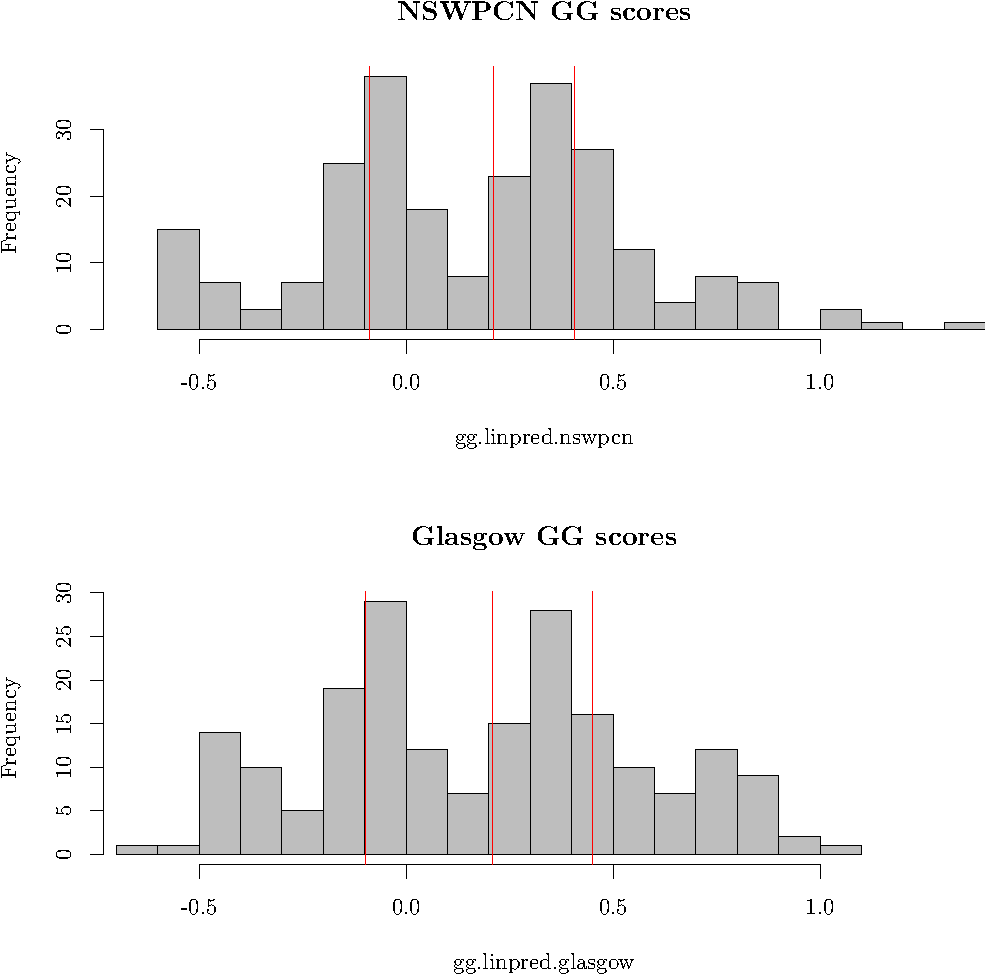
\includegraphics[width=\maxwidth]{figure/05-score-hists-1} 

}


\begin{kframe}\begin{alltt}
\hlkwd{par}\hlstd{(}\hlkwc{mfrow} \hlstd{=} \hlkwd{c}\hlstd{(}\hlnum{1}\hlstd{,} \hlnum{1}\hlstd{))}

\hlkwd{par}\hlstd{(}\hlkwc{mfrow} \hlstd{=} \hlkwd{c}\hlstd{(}\hlnum{2}\hlstd{,} \hlnum{1}\hlstd{))}
\hlkwd{hist}\hlstd{(cph.linpred.nswpcn,} \hlkwc{main} \hlstd{=} \hlstr{"NSWPCN CPH scores"}\hlstd{,} \hlkwc{xlim} \hlstd{=} \hlkwd{range}\hlstd{(}\hlkwd{c}\hlstd{(cph.linpred.nswpcn, cph.linpred.glasgow)),} \hlkwc{breaks} \hlstd{=} \hlnum{20}\hlstd{,} \hlkwc{col} \hlstd{=} \hlstr{"grey"}\hlstd{)}
\hlkwd{abline}\hlstd{(}\hlkwc{v} \hlstd{=} \hlkwd{quantile}\hlstd{(gg.linpred.nswpcn,} \hlkwc{probs} \hlstd{=} \hlkwd{c}\hlstd{(}\hlnum{0.25}\hlstd{,} \hlnum{0.5}\hlstd{,} \hlnum{0.75}\hlstd{)),} \hlkwc{col} \hlstd{=} \hlstr{"red"}\hlstd{)}
\hlkwd{hist}\hlstd{(cph.linpred.glasgow,} \hlkwc{main} \hlstd{=} \hlstr{"Glasgow CPH scores"}\hlstd{,} \hlkwc{xlim} \hlstd{=} \hlkwd{range}\hlstd{(}\hlkwd{c}\hlstd{(cph.linpred.nswpcn, cph.linpred.glasgow)),} \hlkwc{breaks} \hlstd{=} \hlnum{20}\hlstd{,} \hlkwc{col} \hlstd{=} \hlstr{"grey"}\hlstd{)}
\hlkwd{abline}\hlstd{(}\hlkwc{v} \hlstd{=} \hlkwd{quantile}\hlstd{(gg.linpred.glasgow,} \hlkwc{probs} \hlstd{=} \hlkwd{c}\hlstd{(}\hlnum{0.25}\hlstd{,} \hlnum{0.5}\hlstd{,} \hlnum{0.75}\hlstd{)),} \hlkwc{col} \hlstd{=} \hlstr{"red"}\hlstd{)}
\end{alltt}
\end{kframe}

{\centering 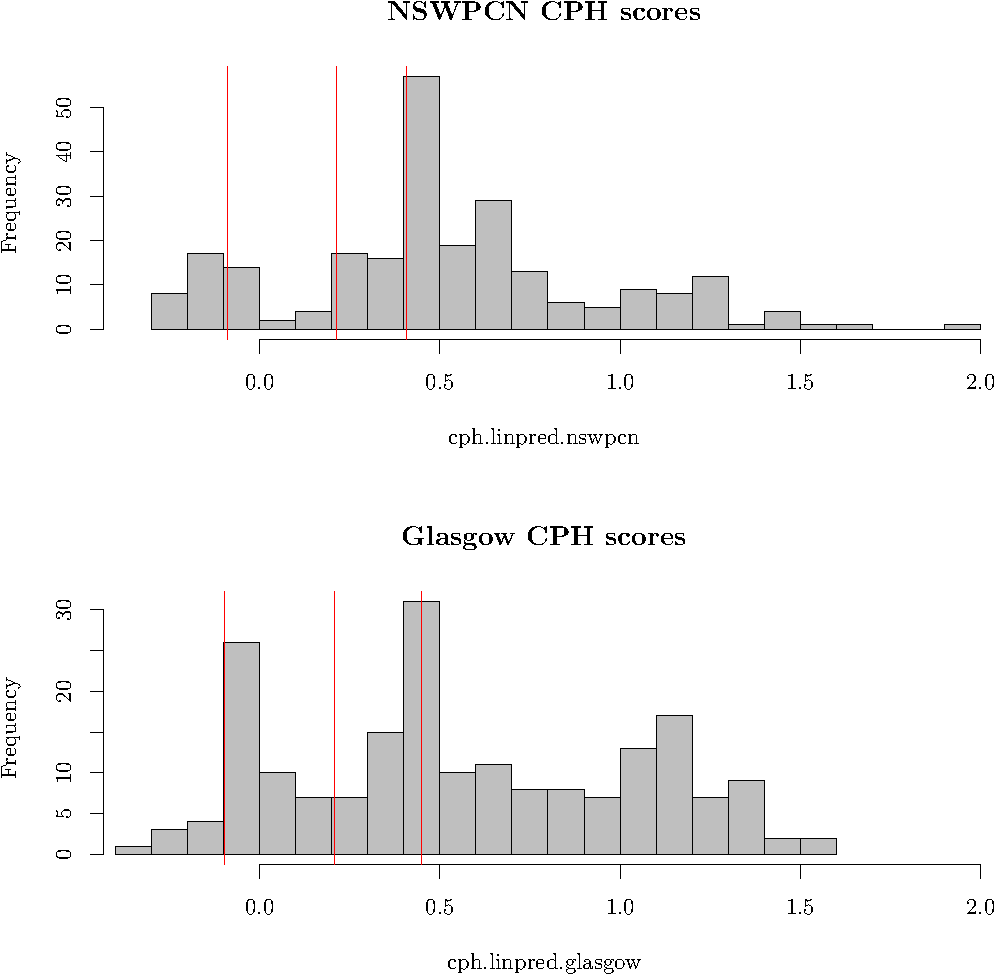
\includegraphics[width=\maxwidth]{figure/05-score-hists-2} 

}


\begin{kframe}\begin{alltt}
\hlkwd{par}\hlstd{(}\hlkwc{mfrow} \hlstd{=} \hlkwd{c}\hlstd{(}\hlnum{1}\hlstd{,} \hlnum{1}\hlstd{))}
\end{alltt}
\end{kframe}
\end{knitrout}

\subsection{Altman method 1 (D,F)}
\begin{knitrout}
\definecolor{shadecolor}{rgb}{0.969, 0.969, 0.969}\color{fgcolor}\begin{kframe}
\begin{alltt}
\hlkwd{summary}\hlstd{(}\hlkwd{coxph}\hlstd{(}\hlkwd{Surv}\hlstd{(Time, DSD)} \hlopt{~} \hlstd{mskcc_post.linpred.glasgow, data.glasgow))}
\end{alltt}
\begin{verbatim}
## Call:
## coxph(formula = Surv(Time, DSD) ~ mskcc_post.linpred.glasgow, 
##     data = data.glasgow)
## 
##   n= 198, number of events= 170 
## 
##                               coef exp(coef) se(coef)    z Pr(>|z|)
## mskcc_post.linpred.glasgow 0.01484   1.01495  0.00405 3.67  0.00025
## 
##                            exp(coef) exp(-coef) lower .95 upper .95
## mskcc_post.linpred.glasgow      1.01      0.985      1.01      1.02
## 
## Concordance= 0.576  (se = 0.025 )
## Rsquare= 0.067   (max possible= 0.999 )
## Likelihood ratio test= 13.6  on 1 df,   p=0.000221
## Wald test            = 13.4  on 1 df,   p=0.000245
## Score (logrank) test = 13.6  on 1 df,   p=0.000229
\end{verbatim}
\begin{alltt}
\hlkwd{summary}\hlstd{(}\hlkwd{coxph}\hlstd{(}\hlkwd{Surv}\hlstd{(Time, DSD)} \hlopt{~} \hlstd{mskcc_pre.linpred.glasgow, data.glasgow))}
\end{alltt}
\begin{verbatim}
## Call:
## coxph(formula = Surv(Time, DSD) ~ mskcc_pre.linpred.glasgow, 
##     data = data.glasgow)
## 
##   n= 198, number of events= 170 
## 
##                                coef exp(coef)  se(coef)     z Pr(>|z|)
## mskcc_pre.linpred.glasgow -0.000423  0.999577  0.007318 -0.06     0.95
## 
##                           exp(coef) exp(-coef) lower .95 upper .95
## mskcc_pre.linpred.glasgow         1          1     0.985      1.01
## 
## Concordance= 0.421  (se = 0.025 )
## Rsquare= 0   (max possible= 0.999 )
## Likelihood ratio test= 0  on 1 df,   p=0.954
## Wald test            = 0  on 1 df,   p=0.954
## Score (logrank) test = 0  on 1 df,   p=0.954
\end{verbatim}
\begin{alltt}
\hlkwd{summary}\hlstd{(}\hlkwd{coxph}\hlstd{(}\hlkwd{Surv}\hlstd{(Time, DSD)} \hlopt{~} \hlstd{gg.linpred.glasgow, data.glasgow))}
\end{alltt}
\begin{verbatim}
## Call:
## coxph(formula = Surv(Time, DSD) ~ gg.linpred.glasgow, data = data.glasgow)
## 
##   n= 198, number of events= 170 
## 
##                     coef exp(coef) se(coef)    z Pr(>|z|)
## gg.linpred.glasgow 0.718     2.051    0.214 3.36  0.00078
## 
##                    exp(coef) exp(-coef) lower .95 upper .95
## gg.linpred.glasgow      2.05      0.488      1.35      3.12
## 
## Concordance= 0.602  (se = 0.025 )
## Rsquare= 0.056   (max possible= 0.999 )
## Likelihood ratio test= 11.3  on 1 df,   p=0.00077
## Wald test            = 11.3  on 1 df,   p=0.000779
## Score (logrank) test = 11.4  on 1 df,   p=0.000738
\end{verbatim}
\begin{alltt}
\hlkwd{summary}\hlstd{(}\hlkwd{coxph}\hlstd{(}\hlkwd{Surv}\hlstd{(Time, DSD)} \hlopt{~} \hlstd{cph.linpred.glasgow, data.glasgow))}
\end{alltt}
\begin{verbatim}
## Call:
## coxph(formula = Surv(Time, DSD) ~ cph.linpred.glasgow, data = data.glasgow)
## 
##   n= 198, number of events= 170 
## 
##                      coef exp(coef) se(coef)    z Pr(>|z|)
## cph.linpred.glasgow 1.012     2.752    0.179 5.66  1.5e-08
## 
##                     exp(coef) exp(-coef) lower .95 upper .95
## cph.linpred.glasgow      2.75      0.363      1.94      3.91
## 
## Concordance= 0.658  (se = 0.025 )
## Rsquare= 0.148   (max possible= 0.999 )
## Likelihood ratio test= 31.6  on 1 df,   p=1.85e-08
## Wald test            = 32.1  on 1 df,   p=1.48e-08
## Score (logrank) test = 33.1  on 1 df,   p=8.54e-09
\end{verbatim}
\begin{alltt}
\hlkwd{anova}\hlstd{(}\hlkwd{coxph}\hlstd{(}\hlkwd{Surv}\hlstd{(Time, DSD)} \hlopt{~} \hlkwd{offset}\hlstd{(gg.linpred.glasgow)} \hlopt{+} \hlstd{gg.linpred.glasgow, data.glasgow))}
\end{alltt}
\begin{verbatim}
## Analysis of Deviance Table
##  Cox model: response is Surv(Time, DSD)
## Terms added sequentially (first to last)
## 
##                    loglik Chisq Df Pr(>|Chi|)
## NULL                 -724                    
## gg.linpred.glasgow   -723  1.73  1       0.19
\end{verbatim}
\begin{alltt}
\hlkwd{anova}\hlstd{(}\hlkwd{coxph}\hlstd{(}\hlkwd{Surv}\hlstd{(Time, DSD)} \hlopt{~} \hlkwd{offset}\hlstd{(cph.linpred.glasgow)} \hlopt{+} \hlstd{cph.linpred.glasgow, data.glasgow))}
\end{alltt}
\begin{verbatim}
## Analysis of Deviance Table
##  Cox model: response is Surv(Time, DSD)
## Terms added sequentially (first to last)
## 
##                     loglik Chisq Df Pr(>|Chi|)
## NULL                  -713                    
## cph.linpred.glasgow   -713     0  1       0.95
\end{verbatim}
\end{kframe}
\end{knitrout}
Booyah.


\subsection{Altman method 2 (F)}
\begin{knitrout}
\definecolor{shadecolor}{rgb}{0.969, 0.969, 0.969}\color{fgcolor}\begin{kframe}
\begin{alltt}
\hlkwd{summary}\hlstd{(}\hlkwd{coxph}\hlstd{(}\hlkwd{Surv}\hlstd{(Time, DSD)} \hlopt{~} \hlkwd{offset}\hlstd{(mskcc_pre.linpred.glasgow)} \hlopt{+} \hlstd{AgeCent} \hlopt{+} \hlstd{SexM} \hlopt{+} \hlstd{SizeCent} \hlopt{+} \hlstd{A2} \hlopt{+} \hlstd{A4, data.glasgow))}
\end{alltt}


{\ttfamily\noindent\color{warningcolor}{\#\# Warning in fitter(X, Y, strats, offset, init, control, weights = weights, : Ran out of iterations and did not converge}}

{\ttfamily\noindent\bfseries\color{errorcolor}{\#\# Error in fitter(X, Y, strats, offset, init, control, weights = weights, : NA/NaN/Inf in foreign function call (arg 6)}}\begin{alltt}
\hlkwd{summary}\hlstd{(}\hlkwd{coxph}\hlstd{(}\hlkwd{Surv}\hlstd{(Time, DSD)} \hlopt{~} \hlkwd{offset}\hlstd{(mskcc_post.linpred.glasgow)} \hlopt{+} \hlstd{AgeCent} \hlopt{+} \hlstd{SexM} \hlopt{+} \hlstd{SizeCent} \hlopt{+} \hlstd{A2} \hlopt{+} \hlstd{A4, data.glasgow))}
\end{alltt}
\begin{verbatim}
## Call:
## coxph(formula = Surv(Time, DSD) ~ offset(mskcc_post.linpred.glasgow) + 
##     AgeCent + SexM + SizeCent + A2 + A4, data = data.glasgow)
## 
##   n= 198, number of events= 170 
## 
##               coef exp(coef)  se(coef)      z Pr(>|z|)
## AgeCent    0.22831   1.25648   0.01006  22.69  < 2e-16
## SexMTRUE  -5.22725   0.00537   0.30189 -17.32  < 2e-16
## SizeCent   0.14973   1.16152   0.01910   7.84  4.6e-15
## A2TRUE    -2.29883   0.10038   0.37880  -6.07  1.3e-09
## A4TRUE     4.93307 138.80556   0.29941  16.48  < 2e-16
## 
##          exp(coef) exp(-coef) lower .95 upper .95
## AgeCent   1.26e+00     0.7959   1.23194    1.2815
## SexMTRUE  5.37e-03   186.2805   0.00297    0.0097
## SizeCent  1.16e+00     0.8609   1.11884    1.2058
## A2TRUE    1.00e-01     9.9625   0.04777    0.2109
## A4TRUE    1.39e+02     0.0072  77.18720  249.6137
## 
## Concordance= 0.587  (se = 0.025 )
## Rsquare= 1   (max possible= 1 )
## Likelihood ratio test= 1719  on 5 df,   p=0
## Wald test            = 2210  on 5 df,   p=0
## Score (logrank) test = 12193  on 5 df,   p=0
\end{verbatim}
\begin{alltt}
\hlkwd{summary}\hlstd{(}\hlkwd{coxph}\hlstd{(}\hlkwd{Surv}\hlstd{(Time, DSD)} \hlopt{~} \hlkwd{offset}\hlstd{(gg.linpred.glasgow)} \hlopt{+} \hlstd{AgeCent} \hlopt{+} \hlstd{SexM} \hlopt{+} \hlstd{SizeCent} \hlopt{+} \hlstd{A2} \hlopt{+} \hlstd{A4, data.glasgow))}
\end{alltt}
\begin{verbatim}
## Call:
## coxph(formula = Surv(Time, DSD) ~ offset(gg.linpred.glasgow) + 
##     AgeCent + SexM + SizeCent + A2 + A4, data = data.glasgow)
## 
##   n= 198, number of events= 170 
## 
##              coef exp(coef) se(coef)     z Pr(>|z|)
## AgeCent  -0.03255   0.96797  0.00860 -3.78  0.00015
## SexMTRUE  0.69598   2.00568  0.16160  4.31  1.7e-05
## SizeCent  0.02457   1.02487  0.00737  3.33  0.00086
## A2TRUE    0.31058   1.36422  0.17387  1.79  0.07406
## A4TRUE   -0.04240   0.95849  0.17723 -0.24  0.81093
## 
##          exp(coef) exp(-coef) lower .95 upper .95
## AgeCent      0.968      1.033     0.952     0.984
## SexMTRUE     2.006      0.499     1.461     2.753
## SizeCent     1.025      0.976     1.010     1.040
## A2TRUE       1.364      0.733     0.970     1.918
## A4TRUE       0.958      1.043     0.677     1.357
## 
## Concordance= 0.681  (se = 0.025 )
## Rsquare= 0.208   (max possible= 0.999 )
## Likelihood ratio test= 46.1  on 5 df,   p=8.58e-09
## Wald test            = 46.9  on 5 df,   p=5.86e-09
## Score (logrank) test = 49.1  on 5 df,   p=2.14e-09
\end{verbatim}
\begin{alltt}
\hlkwd{summary}\hlstd{(}\hlkwd{coxph}\hlstd{(}\hlkwd{Surv}\hlstd{(Time, DSD)} \hlopt{~} \hlkwd{offset}\hlstd{(cph.linpred.glasgow)} \hlopt{+} \hlstd{AgeCent} \hlopt{+} \hlstd{SexM} \hlopt{+} \hlstd{SizeCent} \hlopt{+} \hlstd{A2} \hlopt{+} \hlstd{A4, data.glasgow))}
\end{alltt}
\begin{verbatim}
## Call:
## coxph(formula = Surv(Time, DSD) ~ offset(cph.linpred.glasgow) + 
##     AgeCent + SexM + SizeCent + A2 + A4, data = data.glasgow)
## 
##   n= 198, number of events= 170 
## 
##              coef exp(coef) se(coef)     z Pr(>|z|)
## AgeCent  -0.03255   0.96797  0.00860 -3.78  0.00015
## SexMTRUE  0.26736   1.30651  0.16160  1.65  0.09803
## SizeCent  0.01982   1.02002  0.00737  2.69  0.00719
## A2TRUE    0.10517   1.11090  0.17387  0.60  0.54526
## A4TRUE   -0.15400   0.85728  0.17723 -0.87  0.38489
## 
##          exp(coef) exp(-coef) lower .95 upper .95
## AgeCent      0.968      1.033     0.952     0.984
## SexMTRUE     1.307      0.765     0.952     1.793
## SizeCent     1.020      0.980     1.005     1.035
## A2TRUE       1.111      0.900     0.790     1.562
## A4TRUE       0.857      1.166     0.606     1.213
## 
## Concordance= 0.681  (se = 0.025 )
## Rsquare= 0.114   (max possible= 0.999 )
## Likelihood ratio test= 24.1  on 5 df,   p=0.000211
## Wald test            = 24.9  on 5 df,   p=0.000142
## Score (logrank) test = 25.5  on 5 df,   p=0.000112
\end{verbatim}
\end{kframe}
\end{knitrout}
Still strong evidence of misspecification or poor fit.  However, the above calibration slope was not significantly different from 1.  Hmm.  This doesn't necessarily sink the method, but will need checking as we go along.

\subsection{Altman method 3 (D)}
Look at the CIs above.

\subsection{Altman method 4 (D,C)}
\begin{knitrout}
\definecolor{shadecolor}{rgb}{0.969, 0.969, 0.969}\color{fgcolor}\begin{kframe}
\begin{alltt}
\hlstd{group_quantiles} \hlkwb{=} \hlkwd{c}\hlstd{(}\hlnum{0}\hlstd{,} \hlnum{0.25}\hlstd{,} \hlnum{0.5}\hlstd{,} \hlnum{0.75}\hlstd{,} \hlnum{1}\hlstd{)}
\hlstd{mskcc_pre.groups.glasgow} \hlkwb{=} \hlkwd{cut}\hlstd{(mskcc_pre.linpred.glasgow,} \hlkwd{quantile}\hlstd{(mskcc_pre.linpred.glasgow, group_quantiles))}
\hlstd{mskcc_post.groups.glasgow} \hlkwb{=} \hlkwd{cut}\hlstd{(mskcc_post.linpred.glasgow,} \hlkwd{quantile}\hlstd{(mskcc_post.linpred.glasgow, group_quantiles))}
\hlstd{gg.groups.glasgow} \hlkwb{=} \hlkwd{cut}\hlstd{(gg.linpred.glasgow,} \hlkwd{quantile}\hlstd{(gg.linpred.glasgow, group_quantiles))}
\hlstd{gg.groups.nswpcn} \hlkwb{=} \hlkwd{cut}\hlstd{(gg.linpred.nswpcn,} \hlkwd{quantile}\hlstd{(gg.linpred.nswpcn, group_quantiles))}
\hlstd{cph.groups.glasgow} \hlkwb{=} \hlkwd{cut}\hlstd{(cph.linpred.glasgow,} \hlkwd{quantile}\hlstd{(cph.linpred.glasgow, group_quantiles))}
\hlstd{cph.groups.nswpcn} \hlkwb{=} \hlkwd{cut}\hlstd{(cph.linpred.nswpcn,} \hlkwd{quantile}\hlstd{(cph.linpred.nswpcn, group_quantiles))}

\hlkwd{par}\hlstd{(}\hlkwc{mfrow} \hlstd{=} \hlkwd{c}\hlstd{(}\hlnum{3}\hlstd{,} \hlnum{2}\hlstd{))}
\hlkwd{plot}\hlstd{(}\hlkwd{survfit}\hlstd{(}\hlkwd{Surv}\hlstd{(data.nswpcn}\hlopt{$}\hlstd{Time, data.nswpcn}\hlopt{$}\hlstd{DSD)} \hlopt{~} \hlstd{gg.groups.nswpcn),} \hlkwc{col} \hlstd{=} \hlnum{1}\hlopt{:}\hlstd{(}\hlkwd{length}\hlstd{(group_quantiles)}\hlopt{-}\hlnum{1}\hlstd{),} \hlkwc{xlab} \hlstd{=} \hlstr{"Time (days)"}\hlstd{,} \hlkwc{ylab} \hlstd{=} \hlstr{"Fraction Alive"}\hlstd{,} \hlkwc{main} \hlstd{=} \hlstr{"GG: NSWPCN (Resubstitution)"}\hlstd{)}
\hlkwd{plot}\hlstd{(}\hlkwd{survfit}\hlstd{(}\hlkwd{Surv}\hlstd{(data.glasgow}\hlopt{$}\hlstd{Time, data.glasgow}\hlopt{$}\hlstd{DSD)} \hlopt{~} \hlstd{gg.groups.glasgow),} \hlkwc{col} \hlstd{=} \hlnum{1}\hlopt{:}\hlstd{(}\hlkwd{length}\hlstd{(group_quantiles)}\hlopt{-}\hlnum{1}\hlstd{),} \hlkwc{xlab} \hlstd{=} \hlstr{"Time (days)"}\hlstd{,} \hlkwc{ylab} \hlstd{=} \hlstr{"Fraction Alive"}\hlstd{,} \hlkwc{main} \hlstd{=} \hlstr{"GG: Glasgow"}\hlstd{)}
\hlkwd{plot}\hlstd{(}\hlkwd{survfit}\hlstd{(}\hlkwd{Surv}\hlstd{(data.nswpcn}\hlopt{$}\hlstd{Time, data.nswpcn}\hlopt{$}\hlstd{DSD)} \hlopt{~} \hlstd{cph.groups.nswpcn),} \hlkwc{col} \hlstd{=} \hlnum{1}\hlopt{:}\hlstd{(}\hlkwd{length}\hlstd{(group_quantiles)}\hlopt{-}\hlnum{1}\hlstd{),} \hlkwc{xlab} \hlstd{=} \hlstr{"Time (days)"}\hlstd{,} \hlkwc{ylab} \hlstd{=} \hlstr{"Fraction Alive"}\hlstd{,} \hlkwc{main} \hlstd{=} \hlstr{"CPH: NSWPCN (Resubstitution)"}\hlstd{)}
\hlkwd{plot}\hlstd{(}\hlkwd{survfit}\hlstd{(}\hlkwd{Surv}\hlstd{(data.glasgow}\hlopt{$}\hlstd{Time, data.glasgow}\hlopt{$}\hlstd{DSD)} \hlopt{~} \hlstd{cph.groups.glasgow),} \hlkwc{col} \hlstd{=} \hlnum{1}\hlopt{:}\hlstd{(}\hlkwd{length}\hlstd{(group_quantiles)}\hlopt{-}\hlnum{1}\hlstd{),} \hlkwc{xlab} \hlstd{=} \hlstr{"Time (days)"}\hlstd{,} \hlkwc{ylab} \hlstd{=} \hlstr{"Fraction Alive"}\hlstd{,} \hlkwc{main} \hlstd{=} \hlstr{"CPH: Glasgow"}\hlstd{)}
\hlkwd{plot}\hlstd{(}\hlkwd{survfit}\hlstd{(}\hlkwd{Surv}\hlstd{(data.glasgow}\hlopt{$}\hlstd{Time, data.glasgow}\hlopt{$}\hlstd{DSD)} \hlopt{~} \hlstd{mskcc_pre.groups.glasgow),} \hlkwc{col} \hlstd{=} \hlnum{1}\hlopt{:}\hlstd{(}\hlkwd{length}\hlstd{(group_quantiles)}\hlopt{-}\hlnum{1}\hlstd{),} \hlkwc{xlab} \hlstd{=} \hlstr{"Time (days)"}\hlstd{,} \hlkwc{ylab} \hlstd{=} \hlstr{"Fraction Alive"}\hlstd{,} \hlkwc{main} \hlstd{=} \hlstr{"MSKCC Preop: Glasgow"}\hlstd{)}
\hlkwd{plot}\hlstd{(}\hlkwd{survfit}\hlstd{(}\hlkwd{Surv}\hlstd{(data.glasgow}\hlopt{$}\hlstd{Time, data.glasgow}\hlopt{$}\hlstd{DSD)} \hlopt{~} \hlstd{mskcc_post.groups.glasgow),} \hlkwc{col} \hlstd{=} \hlnum{1}\hlopt{:}\hlstd{(}\hlkwd{length}\hlstd{(group_quantiles)}\hlopt{-}\hlnum{1}\hlstd{),} \hlkwc{xlab} \hlstd{=} \hlstr{"Time (days)"}\hlstd{,} \hlkwc{ylab} \hlstd{=} \hlstr{"Fraction Alive"}\hlstd{,} \hlkwc{main} \hlstd{=} \hlstr{"MSKCC Postop: Glasgow"}\hlstd{)}
\end{alltt}
\end{kframe}

{\centering 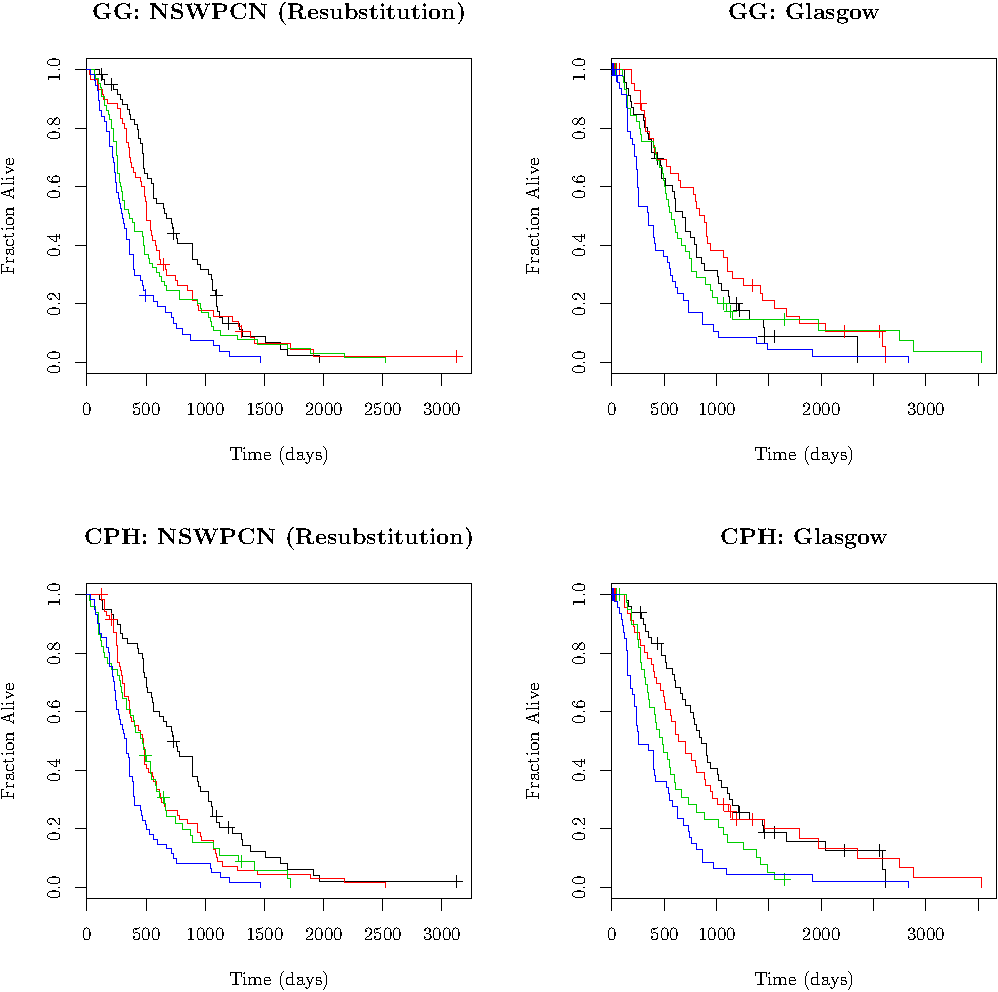
\includegraphics[width=\maxwidth]{figure/05-altman-4-1} 

}


\begin{kframe}\begin{alltt}
\hlkwd{par}\hlstd{(}\hlkwc{mfrow} \hlstd{=} \hlkwd{c}\hlstd{(}\hlnum{1}\hlstd{,} \hlnum{1}\hlstd{))}

\hlcom{# temp = survfit(Surv(data.nswpcn$Time, data.nswpcn$DSD) ~ gg.groups.nswpcn)}
\hlcom{# plot(0 ~ 0, type = "n", xlim = c(0, max(data.nswpcn$Time)), ylim = c(0, 1))}
\hlcom{# for (i in )}
\end{alltt}
\end{kframe}
\end{knitrout}
Weird.  MSKCC somehow is still finding a subgroup, and it's somehow even clearer in preop!  This is based on an approximation to GG only, but should be pretty close.  It certainly does OK on resubstituted data, but not so well on the Glasgow patients.


\subsection{Brier score}
\begin{knitrout}
\definecolor{shadecolor}{rgb}{0.969, 0.969, 0.969}\color{fgcolor}\begin{kframe}
\begin{alltt}
\hlstd{calcIBS} \hlkwb{=} \hlkwa{function}\hlstd{(}\hlkwc{surv}\hlstd{,} \hlkwc{pred}\hlstd{,} \hlkwc{pred_times}\hlstd{,} \hlkwc{max_time}\hlstd{)}
\hlstd{\{}
        \hlkwd{stopifnot}\hlstd{(}\hlkwd{nrow}\hlstd{(surv)} \hlopt{==} \hlkwd{nrow}\hlstd{(pred)} \hlopt{&&} \hlkwd{length}\hlstd{(pred_times)} \hlopt{==} \hlkwd{ncol}\hlstd{(pred))}

        \hlstd{n} \hlkwb{=} \hlkwd{nrow}\hlstd{(surv)}
        \hlstd{marg_survfit} \hlkwb{=} \hlkwd{survfit}\hlstd{(surv} \hlopt{~} \hlnum{1}\hlstd{)}
        \hlstd{marg_censfit} \hlkwb{=} \hlkwd{survfit}\hlstd{(}\hlkwd{Surv}\hlstd{(surv[,}\hlnum{1}\hlstd{],} \hlopt{!}\hlstd{surv[,}\hlnum{2}\hlstd{])} \hlopt{~} \hlnum{1}\hlstd{)}
        \hlstd{marg_surv_func} \hlkwb{=} \hlkwd{approxfun}\hlstd{(marg_survfit}\hlopt{$}\hlstd{time, marg_survfit}\hlopt{$}\hlstd{surv,} \hlkwc{method} \hlstd{=} \hlstr{"constant"}\hlstd{,} \hlkwc{yleft} \hlstd{=} \hlnum{1}\hlstd{,} \hlkwc{yright} \hlstd{=} \hlnum{0}\hlstd{,} \hlkwc{rule} \hlstd{=} \hlnum{2}\hlopt{:}\hlnum{1}\hlstd{,} \hlkwc{f} \hlstd{=} \hlnum{0}\hlstd{)}
        \hlstd{marg_cens_func} \hlkwb{=} \hlkwd{approxfun}\hlstd{(marg_censfit}\hlopt{$}\hlstd{time, marg_censfit}\hlopt{$}\hlstd{surv,} \hlkwc{method} \hlstd{=} \hlstr{"constant"}\hlstd{,} \hlkwc{yleft} \hlstd{=} \hlnum{1}\hlstd{,} \hlkwc{yright} \hlstd{=} \hlnum{0}\hlstd{,} \hlkwc{rule} \hlstd{=} \hlnum{2}\hlopt{:}\hlnum{1}\hlstd{,} \hlkwc{f} \hlstd{=} \hlnum{0}\hlstd{)}

        \hlstd{pred_funcs} \hlkwb{=} \hlkwd{apply}\hlstd{(pred,} \hlnum{1}\hlstd{,} \hlkwa{function}\hlstd{(}\hlkwc{pat_preds}\hlstd{)} \hlkwd{approxfun}\hlstd{(pred_times, pat_preds,} \hlkwc{yleft} \hlstd{=} \hlnum{1}\hlstd{,} \hlkwc{yright} \hlstd{=} \hlkwd{min}\hlstd{(pat_preds),} \hlkwc{rule} \hlstd{=} \hlnum{2}\hlstd{))}

        \hlstd{indiv_patient_bsc} \hlkwb{=} \hlkwa{function}\hlstd{(}\hlkwc{pat_i}\hlstd{,} \hlkwc{tstars}\hlstd{)}
        \hlstd{\{}
                \hlstd{observed_time} \hlkwb{=} \hlstd{surv[pat_i,} \hlnum{1}\hlstd{]}
                \hlstd{observed_event} \hlkwb{=} \hlstd{surv[pat_i,} \hlnum{2}\hlstd{]}
                \hlstd{pred_func} \hlkwb{=} \hlstd{pred_funcs[[pat_i]]}
                \hlstd{category} \hlkwb{=} \hlnum{1}\hlopt{*}\hlstd{(observed_time} \hlopt{<=} \hlstd{tstars} \hlopt{&} \hlstd{observed_event)} \hlopt{+} \hlnum{2}\hlopt{*}\hlstd{(observed_time} \hlopt{>} \hlstd{tstars)} \hlopt{+} \hlnum{3}\hlopt{*}\hlstd{(observed_time} \hlopt{<=} \hlstd{tstars} \hlopt{& !}\hlstd{observed_event)}
                \hlstd{bsc} \hlkwb{=} \hlkwd{rep}\hlstd{(}\hlnum{NA}\hlstd{,} \hlkwd{length}\hlstd{(tstars))}
                \hlstd{bsc[category} \hlopt{==} \hlnum{1}\hlstd{]} \hlkwb{=} \hlkwd{pred_func}\hlstd{(tstars[category} \hlopt{==} \hlnum{1}\hlstd{])}\hlopt{^}\hlnum{2} \hlopt{/} \hlkwd{marg_cens_func}\hlstd{(observed_time)}
                \hlstd{bsc[category} \hlopt{==} \hlnum{2}\hlstd{]} \hlkwb{=} \hlstd{(}\hlnum{1} \hlopt{-} \hlkwd{pred_func}\hlstd{(tstars[category} \hlopt{==} \hlnum{2}\hlstd{]))}\hlopt{^}\hlnum{2} \hlopt{/} \hlkwd{marg_cens_func}\hlstd{(tstars[category} \hlopt{==} \hlnum{2}\hlstd{])}
                \hlstd{bsc[category} \hlopt{==} \hlnum{3}\hlstd{]} \hlkwb{=} \hlnum{0}
                \hlstd{bsc}
        \hlstd{\}}

        \hlstd{bsc_func} \hlkwb{=} \hlkwa{function}\hlstd{(}\hlkwc{tstars}\hlstd{) \{} \hlkwd{rowMeans}\hlstd{(}\hlkwd{sapply}\hlstd{(}\hlnum{1}\hlopt{:}\hlstd{n,} \hlkwa{function}\hlstd{(}\hlkwc{pat_i}\hlstd{)} \hlkwd{indiv_patient_bsc}\hlstd{(pat_i, tstars))) \}}

        \hlstd{weight_func} \hlkwb{=} \hlkwa{function}\hlstd{(}\hlkwc{tstars}\hlstd{) \{ (}\hlnum{1} \hlopt{-} \hlkwd{marg_surv_func}\hlstd{(tstars))} \hlopt{/} \hlstd{(}\hlnum{1} \hlopt{-} \hlkwd{marg_surv_func}\hlstd{(max_time)) \}}

        \hlcom{# Be slack and do trapezoidal int. with a fine grid.  It should be possible }
        \hlcom{# to calulate the int. exactly but I cbfed.}
        \hlstd{int_grid} \hlkwb{=} \hlkwd{seq}\hlstd{(}\hlnum{0}\hlstd{, max_time,} \hlkwc{length.out} \hlstd{=} \hlnum{1e3}\hlstd{)}
        \hlstd{bsc_vals} \hlkwb{=} \hlkwd{bsc_func}\hlstd{(int_grid)}
        \hlstd{weight_vals} \hlkwb{=} \hlkwd{weight_func}\hlstd{(int_grid)}
        \hlstd{int_vals} \hlkwb{=} \hlstd{bsc_vals} \hlopt{*} \hlstd{weight_vals}
        \hlstd{ibsc} \hlkwb{=} \hlstd{(}\hlnum{2}\hlopt{*}\hlkwd{sum}\hlstd{(int_vals)} \hlopt{-} \hlstd{int_vals[}\hlnum{1}\hlstd{]} \hlopt{-} \hlstd{int_vals[}\hlkwd{length}\hlstd{(int_vals)])} \hlopt{*} \hlstd{(}\hlkwd{diff}\hlstd{(}\hlkwd{range}\hlstd{(int_grid)))} \hlopt{/} \hlstd{(}\hlnum{2}\hlopt{*}\hlkwd{length}\hlstd{(int_vals))}

        \hlkwd{return}\hlstd{(}\hlkwd{list}\hlstd{(}\hlkwc{bsc} \hlstd{= bsc_vals,} \hlkwc{weights} \hlstd{= weight_vals,} \hlkwc{eval_times} \hlstd{= int_grid,} \hlkwc{ibsc} \hlstd{= ibsc))}
\hlstd{\}}

\hlstd{calcBSsingle} \hlkwb{=} \hlkwa{function}\hlstd{(}\hlkwc{surv}\hlstd{,} \hlkwc{pred}\hlstd{,} \hlkwc{pred_time}\hlstd{)}
\hlstd{\{}
        \hlstd{n} \hlkwb{=} \hlkwd{nrow}\hlstd{(surv)}
        \hlstd{obs_time} \hlkwb{=} \hlstd{surv[,}\hlnum{1}\hlstd{]}
        \hlstd{obs_event} \hlkwb{=} \hlstd{surv[,}\hlnum{2}\hlstd{]}
        \hlstd{marg_censfit} \hlkwb{=} \hlkwd{survfit}\hlstd{(}\hlkwd{Surv}\hlstd{(obs_time,} \hlopt{!}\hlstd{obs_event)} \hlopt{~} \hlnum{1}\hlstd{)}
        \hlstd{marg_cens_func} \hlkwb{=} \hlkwd{approxfun}\hlstd{(marg_censfit}\hlopt{$}\hlstd{time, marg_censfit}\hlopt{$}\hlstd{surv,} \hlkwc{method} \hlstd{=} \hlstr{"constant"}\hlstd{,} \hlkwc{yleft} \hlstd{=} \hlnum{1}\hlstd{,} \hlkwc{yright} \hlstd{=} \hlnum{0}\hlstd{,} \hlkwc{rule} \hlstd{=} \hlnum{2}\hlopt{:}\hlnum{1}\hlstd{,} \hlkwc{f} \hlstd{=} \hlnum{0}\hlstd{)}

        \hlstd{brier_val} \hlkwb{=} \hlkwd{rep}\hlstd{(}\hlnum{NA}\hlstd{, n)}
        \hlstd{cat} \hlkwb{=} \hlnum{1}\hlopt{*}\hlkwd{I}\hlstd{(obs_time} \hlopt{<=} \hlstd{pred_time} \hlopt{&} \hlstd{obs_event)} \hlopt{+} \hlnum{2}\hlopt{*}\hlkwd{I}\hlstd{(obs_time} \hlopt{>} \hlstd{pred_time)} \hlopt{+} \hlnum{3}\hlopt{*}\hlkwd{I}\hlstd{(obs_time} \hlopt{<=} \hlstd{pred_time} \hlopt{& !}\hlstd{obs_event)}
        \hlstd{brier_val[cat} \hlopt{==} \hlnum{1}\hlstd{]} \hlkwb{=} \hlstd{(pred[cat} \hlopt{==} \hlnum{1}\hlstd{])}\hlopt{^}\hlnum{2} \hlopt{/} \hlkwd{marg_cens_func}\hlstd{(obs_time[cat} \hlopt{==} \hlnum{1}\hlstd{])}
        \hlstd{brier_val[cat} \hlopt{==} \hlnum{2}\hlstd{]} \hlkwb{=} \hlstd{(}\hlnum{1}\hlopt{-}\hlstd{pred[cat} \hlopt{==} \hlnum{2}\hlstd{])}\hlopt{^}\hlnum{2} \hlopt{/} \hlkwd{marg_cens_func}\hlstd{(pred_time)}
        \hlstd{brier_val[cat} \hlopt{==} \hlnum{3}\hlstd{]} \hlkwb{=} \hlnum{0}

        \hlkwd{mean}\hlstd{(brier_val)}
\hlstd{\}}
\end{alltt}
\end{kframe}
\end{knitrout}


\begin{knitrout}
\definecolor{shadecolor}{rgb}{0.969, 0.969, 0.969}\color{fgcolor}\begin{kframe}
\begin{alltt}
\hlstd{mskcc_post.12mo.glasgow.brier} \hlkwb{=} \hlkwd{calcBSsingle}\hlstd{(}\hlkwd{Surv}\hlstd{(data.glasgow}\hlopt{$}\hlstd{Time, data.glasgow}\hlopt{$}\hlstd{DSD), mskcc_post.12mo.glasgow,} \hlnum{12}\hlopt{/}\hlnum{12}\hlopt{*}\hlnum{365.25}\hlstd{)}
\hlstd{mskcc_post.24mo.glasgow.brier} \hlkwb{=} \hlkwd{calcBSsingle}\hlstd{(}\hlkwd{Surv}\hlstd{(data.glasgow}\hlopt{$}\hlstd{Time, data.glasgow}\hlopt{$}\hlstd{DSD), mskcc_post.24mo.glasgow,} \hlnum{24}\hlopt{/}\hlnum{12}\hlopt{*}\hlnum{365.25}\hlstd{)}
\hlstd{mskcc_post.36mo.glasgow.brier} \hlkwb{=} \hlkwd{calcBSsingle}\hlstd{(}\hlkwd{Surv}\hlstd{(data.glasgow}\hlopt{$}\hlstd{Time, data.glasgow}\hlopt{$}\hlstd{DSD), mskcc_post.36mo.glasgow,} \hlnum{36}\hlopt{/}\hlnum{12}\hlopt{*}\hlnum{365.25}\hlstd{)}
\hlstd{mskcc_pre.12mo.glasgow.brier} \hlkwb{=} \hlkwd{calcBSsingle}\hlstd{(}\hlkwd{Surv}\hlstd{(data.glasgow}\hlopt{$}\hlstd{Time, data.glasgow}\hlopt{$}\hlstd{DSD), mskcc_pre.12mo.glasgow,} \hlnum{12}\hlopt{/}\hlnum{12}\hlopt{*}\hlnum{365.25}\hlstd{)}
\hlstd{mskcc_pre.24mo.glasgow.brier} \hlkwb{=} \hlkwd{calcBSsingle}\hlstd{(}\hlkwd{Surv}\hlstd{(data.glasgow}\hlopt{$}\hlstd{Time, data.glasgow}\hlopt{$}\hlstd{DSD), mskcc_pre.24mo.glasgow,} \hlnum{24}\hlopt{/}\hlnum{12}\hlopt{*}\hlnum{365.25}\hlstd{)}
\hlstd{mskcc_pre.36mo.glasgow.brier} \hlkwb{=} \hlkwd{calcBSsingle}\hlstd{(}\hlkwd{Surv}\hlstd{(data.glasgow}\hlopt{$}\hlstd{Time, data.glasgow}\hlopt{$}\hlstd{DSD), mskcc_pre.36mo.glasgow,} \hlnum{36}\hlopt{/}\hlnum{12}\hlopt{*}\hlnum{365.25}\hlstd{)}
\hlstd{gg.path.glasgow.brier} \hlkwb{=} \hlkwd{calcIBS}\hlstd{(}\hlkwd{Surv}\hlstd{(data.glasgow}\hlopt{$}\hlstd{Time, data.glasgow}\hlopt{$}\hlstd{DSD),} \hlkwd{t}\hlstd{(}\hlkwd{sapply}\hlstd{(gg.path.glasgow,} \hlkwa{function}\hlstd{(}\hlkwc{x}\hlstd{) x[,}\hlnum{2}\hlstd{])), gg.path.glasgow[[}\hlnum{1}\hlstd{]][,}\hlnum{1}\hlstd{],} \hlnum{10}\hlopt{*}\hlnum{365.25}\hlstd{)}

\hlstd{km0.path.glasgow.brier} \hlkwb{=} \hlkwd{calcIBS}\hlstd{(}\hlkwd{Surv}\hlstd{(data.glasgow}\hlopt{$}\hlstd{Time, data.glasgow}\hlopt{$}\hlstd{DSD),} \hlkwd{matrix}\hlstd{(fit.km0}\hlopt{$}\hlstd{surv,} \hlkwc{nrow} \hlstd{=} \hlkwd{nrow}\hlstd{(data.glasgow),} \hlkwc{ncol} \hlstd{=} \hlkwd{length}\hlstd{(fit.km0}\hlopt{$}\hlstd{time),} \hlkwc{byrow} \hlstd{=} \hlnum{TRUE}\hlstd{), fit.km0}\hlopt{$}\hlstd{time,} \hlnum{10}\hlopt{*}\hlnum{365.25}\hlstd{)}

\hlstd{temp.cph.pred} \hlkwb{=} \hlkwd{survfit}\hlstd{(fit.cph,} \hlkwc{newdata} \hlstd{= data.glasgow)}
\hlstd{temp.cph.pred.expanded_strata} \hlkwb{=} \hlkwd{rep}\hlstd{(}\hlkwd{names}\hlstd{(temp.cph.pred}\hlopt{$}\hlstd{strata), temp.cph.pred}\hlopt{$}\hlstd{strata)}
\hlstd{temp.cph.pred_funcs} \hlkwb{=} \hlkwd{sapply}\hlstd{(}\hlkwd{rownames}\hlstd{(data.glasgow),} \hlkwa{function}\hlstd{(}\hlkwc{pat_id}\hlstd{) \{}
        \hlkwd{approxfun}\hlstd{(temp.cph.pred}\hlopt{$}\hlstd{time[temp.cph.pred.expanded_strata} \hlopt{==} \hlstd{pat_id], temp.cph.pred}\hlopt{$}\hlstd{surv[temp.cph.pred.expanded_strata} \hlopt{==} \hlstd{pat_id],} \hlkwc{method} \hlstd{=} \hlstr{"constant"}\hlstd{,} \hlkwc{f} \hlstd{=} \hlnum{0}\hlstd{,} \hlkwc{yleft} \hlstd{=} \hlnum{1}\hlstd{,} \hlkwc{rule} \hlstd{=} \hlnum{2}\hlstd{)}
\hlstd{\})}
\hlstd{cph.path.glasgow.brier} \hlkwb{=} \hlkwd{calcIBS}\hlstd{(}\hlkwd{Surv}\hlstd{(data.glasgow}\hlopt{$}\hlstd{Time, data.glasgow}\hlopt{$}\hlstd{DSD),}
        \hlkwd{t}\hlstd{(}\hlkwd{sapply}\hlstd{(temp.cph.pred_funcs[}\hlkwd{rownames}\hlstd{(data.glasgow)],} \hlkwa{function}\hlstd{(}\hlkwc{f}\hlstd{)} \hlkwd{f}\hlstd{(}\hlkwd{c}\hlstd{(}\hlnum{12}\hlstd{,} \hlnum{24}\hlstd{,} \hlnum{36}\hlstd{)}\hlopt{/}\hlnum{12}\hlopt{*}\hlnum{365.25}\hlstd{))),} \hlkwd{c}\hlstd{(}\hlnum{12}\hlstd{,} \hlnum{24}\hlstd{,} \hlnum{36}\hlstd{)}\hlopt{/}\hlnum{12}\hlopt{*}\hlnum{365.25}\hlstd{,} \hlnum{10}\hlopt{*}\hlnum{365.25}\hlstd{)}

\hlstd{gg2.path.glasgow.brier} \hlkwb{=} \hlkwd{calcIBS}\hlstd{(}\hlkwd{Surv}\hlstd{(data.glasgow}\hlopt{$}\hlstd{Time, data.glasgow}\hlopt{$}\hlstd{DSD),} \hlkwd{t}\hlstd{(}\hlkwd{sapply}\hlstd{(gg2.path.glasgow,} \hlkwa{function}\hlstd{(}\hlkwc{x}\hlstd{) x[,}\hlnum{2}\hlstd{])), gg2.path.glasgow[[}\hlnum{1}\hlstd{]][,}\hlnum{1}\hlstd{],} \hlnum{10}\hlopt{*}\hlnum{365.25}\hlstd{)}

\hlstd{temp.rsf.pred} \hlkwb{=} \hlkwd{predict}\hlstd{(fit.rsf,} \hlkwc{newdata} \hlstd{= data.glasgow)}
\hlstd{rsf.path.glasgow.brier} \hlkwb{=} \hlkwd{calcIBS}\hlstd{(}\hlkwd{Surv}\hlstd{(data.glasgow}\hlopt{$}\hlstd{Time, data.glasgow}\hlopt{$}\hlstd{DSD),} \hlkwd{t}\hlstd{(}\hlkwd{apply}\hlstd{(temp.rsf.pred}\hlopt{$}\hlstd{survival,} \hlnum{1}\hlstd{,} \hlkwa{function}\hlstd{(}\hlkwc{patpreds}\hlstd{)} \hlkwd{approx}\hlstd{(temp.rsf.pred}\hlopt{$}\hlstd{time.interest, patpreds,} \hlkwd{c}\hlstd{(}\hlnum{12}\hlstd{,} \hlnum{24}\hlstd{,} \hlnum{36}\hlstd{)}\hlopt{/}\hlnum{12}\hlopt{*}\hlnum{365.25}\hlstd{)}\hlopt{$}\hlstd{y)),} \hlkwd{c}\hlstd{(}\hlnum{12}\hlstd{,} \hlnum{24}\hlstd{,} \hlnum{36}\hlstd{)}\hlopt{/}\hlnum{12}\hlopt{*}\hlnum{365.25}\hlstd{,} \hlnum{10}\hlopt{*}\hlnum{365.25}\hlstd{)}

\hlkwd{plot}\hlstd{(gg.path.glasgow.brier}\hlopt{$}\hlstd{bsc} \hlopt{~} \hlstd{gg.path.glasgow.brier}\hlopt{$}\hlstd{eval_times,} \hlkwc{col} \hlstd{=} \hlstr{"aquamarine"}\hlstd{,} \hlkwc{type} \hlstd{=} \hlstr{"l"}\hlstd{,} \hlkwc{ylim} \hlstd{=} \hlkwd{c}\hlstd{(}\hlnum{0}\hlstd{,} \hlnum{0.3}\hlstd{),} \hlkwc{xlab} \hlstd{=} \hlstr{"Time from diagnosis"}\hlstd{,} \hlkwc{ylab} \hlstd{=} \hlstr{"Brier score"}\hlstd{)}
\hlkwd{lines}\hlstd{(km0.path.glasgow.brier}\hlopt{$}\hlstd{bsc} \hlopt{~} \hlstd{km0.path.glasgow.brier}\hlopt{$}\hlstd{eval_times,} \hlkwc{col} \hlstd{=} \hlstr{"grey"}\hlstd{)}
\hlkwd{lines}\hlstd{(cph.path.glasgow.brier}\hlopt{$}\hlstd{bsc} \hlopt{~} \hlstd{cph.path.glasgow.brier}\hlopt{$}\hlstd{eval_times,} \hlkwc{col} \hlstd{=} \hlstr{"pink"}\hlstd{)}
\hlkwd{lines}\hlstd{(gg2.path.glasgow.brier}\hlopt{$}\hlstd{bsc} \hlopt{~} \hlstd{gg2.path.glasgow.brier}\hlopt{$}\hlstd{eval_times,} \hlkwc{col} \hlstd{=} \hlstr{"purple"}\hlstd{)}
\hlkwd{lines}\hlstd{(rsf.path.glasgow.brier}\hlopt{$}\hlstd{bsc} \hlopt{~} \hlstd{rsf.path.glasgow.brier}\hlopt{$}\hlstd{eval_times,} \hlkwc{col} \hlstd{=} \hlstr{"green"}\hlstd{)}
\hlkwd{points}\hlstd{(}\hlkwd{c}\hlstd{(}\hlnum{12}\hlstd{,} \hlnum{24}\hlstd{,} \hlnum{36}\hlstd{)}\hlopt{/}\hlnum{12}\hlopt{*}\hlnum{365.25}\hlstd{,} \hlkwd{c}\hlstd{(mskcc_post.12mo.glasgow.brier, mskcc_post.24mo.glasgow.brier, mskcc_post.36mo.glasgow.brier),} \hlkwc{col} \hlstd{=} \hlstr{"red"}\hlstd{,} \hlkwc{cex} \hlstd{=} \hlnum{1}\hlstd{)}
\hlkwd{points}\hlstd{(}\hlkwd{c}\hlstd{(}\hlnum{12}\hlstd{,} \hlnum{24}\hlstd{,} \hlnum{36}\hlstd{)}\hlopt{/}\hlnum{12}\hlopt{*}\hlnum{365.25}\hlstd{,} \hlkwd{c}\hlstd{(mskcc_pre.12mo.glasgow.brier, mskcc_pre.24mo.glasgow.brier, mskcc_pre.36mo.glasgow.brier),} \hlkwc{col} \hlstd{=} \hlstr{"blue"}\hlstd{,} \hlkwc{cex} \hlstd{=} \hlnum{1}\hlstd{)}
\hlkwd{abline}\hlstd{(}\hlkwc{h} \hlstd{=} \hlnum{0.25}\hlstd{,} \hlkwc{col} \hlstd{=} \hlstr{"grey"}\hlstd{,} \hlkwc{lty} \hlstd{=} \hlstr{"dotted"}\hlstd{)}
\hlkwd{legend}\hlstd{(}\hlstr{"topright"}\hlstd{,}
        \hlkwc{legend} \hlstd{=} \hlkwd{c}\hlstd{(}     \hlstr{"GG1 Preop"}\hlstd{,}    \hlstr{"GG2 Preop"}\hlstd{,}    \hlstr{"CP1 Preop"}\hlstd{,}    \hlstr{"RSF Preop"}\hlstd{,}    \hlstr{"KM0"}\hlstd{,}          \hlstr{"MSKCC Postop"}\hlstd{,}         \hlstr{"MSKCC Preop"}\hlstd{),}
        \hlkwc{pch} \hlstd{=} \hlkwd{c}\hlstd{(}        \hlnum{NA}\hlstd{,}                     \hlnum{NA}\hlstd{,}                     \hlnum{NA}\hlstd{,}                     \hlnum{NA}\hlstd{,}                     \hlnum{NA}\hlstd{,}             \hlnum{1}\hlstd{,}                                      \hlnum{1}\hlstd{),}
        \hlkwc{col} \hlstd{=} \hlkwd{c}\hlstd{(}        \hlstr{"aquamarine"}\hlstd{,}   \hlstr{"purple"}\hlstd{,}               \hlstr{"pink"}\hlstd{,}                 \hlstr{"green"}\hlstd{,}                \hlstr{"grey"}\hlstd{,}         \hlstr{"red"}\hlstd{,}                          \hlstr{"blue"}\hlstd{),}
        \hlkwc{lty} \hlstd{=} \hlkwd{c}\hlstd{(}        \hlstr{"solid"}\hlstd{,}                \hlstr{"solid"}\hlstd{,}                \hlstr{"solid"}\hlstd{,}                \hlstr{"solid"}\hlstd{,}                \hlstr{"solid"}\hlstd{,}        \hlnum{NA}\hlstd{,}                             \hlnum{NA}\hlstd{),}
        \hlkwc{inset} \hlstd{=} \hlnum{0.05}\hlstd{)}
\end{alltt}
\end{kframe}

{\centering 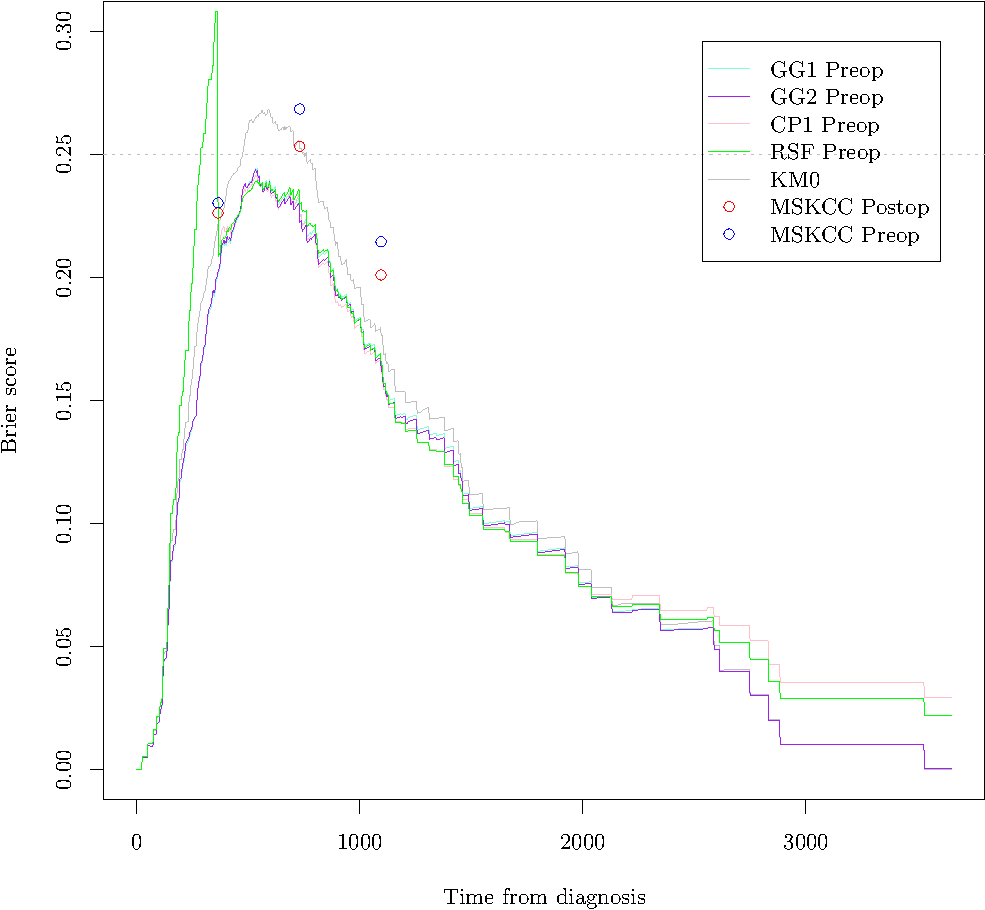
\includegraphics[width=\maxwidth]{figure/05-prob-bs-paths-1} 

}



\end{knitrout}


\begin{knitrout}
\definecolor{shadecolor}{rgb}{0.969, 0.969, 0.969}\color{fgcolor}\begin{kframe}
\begin{alltt}
\hlstd{probs_bs_boot_func} \hlkwb{=} \hlkwa{function}\hlstd{(}\hlkwc{d}\hlstd{,} \hlkwc{i}\hlstd{) \{}
        \hlstd{bs.mskcc.postop.12} \hlkwb{=} \hlkwd{calcBSsingle}\hlstd{(}\hlkwd{Surv}\hlstd{(d}\hlopt{$}\hlstd{Time[i], d}\hlopt{$}\hlstd{DSD[i]), mskcc_post.12mo.glasgow[i],} \hlnum{12}\hlopt{/}\hlnum{12}\hlopt{*}\hlnum{365.25}\hlstd{)}
        \hlstd{bs.mskcc.postop.24} \hlkwb{=} \hlkwd{calcBSsingle}\hlstd{(}\hlkwd{Surv}\hlstd{(d}\hlopt{$}\hlstd{Time[i], d}\hlopt{$}\hlstd{DSD[i]), mskcc_post.24mo.glasgow[i],} \hlnum{24}\hlopt{/}\hlnum{12}\hlopt{*}\hlnum{365.25}\hlstd{)}
        \hlstd{bs.mskcc.postop.36} \hlkwb{=} \hlkwd{calcBSsingle}\hlstd{(}\hlkwd{Surv}\hlstd{(d}\hlopt{$}\hlstd{Time[i], d}\hlopt{$}\hlstd{DSD[i]), mskcc_post.36mo.glasgow[i],} \hlnum{36}\hlopt{/}\hlnum{12}\hlopt{*}\hlnum{365.25}\hlstd{)}
        \hlstd{bs.mskcc.preop.12} \hlkwb{=} \hlkwd{calcBSsingle}\hlstd{(}\hlkwd{Surv}\hlstd{(d}\hlopt{$}\hlstd{Time[i], d}\hlopt{$}\hlstd{DSD[i]), mskcc_pre.12mo.glasgow[i],} \hlnum{12}\hlopt{/}\hlnum{12}\hlopt{*}\hlnum{365.25}\hlstd{)}
        \hlstd{bs.mskcc.preop.24} \hlkwb{=} \hlkwd{calcBSsingle}\hlstd{(}\hlkwd{Surv}\hlstd{(d}\hlopt{$}\hlstd{Time[i], d}\hlopt{$}\hlstd{DSD[i]), mskcc_pre.24mo.glasgow[i],} \hlnum{24}\hlopt{/}\hlnum{12}\hlopt{*}\hlnum{365.25}\hlstd{)}
        \hlstd{bs.mskcc.preop.36} \hlkwb{=} \hlkwd{calcBSsingle}\hlstd{(}\hlkwd{Surv}\hlstd{(d}\hlopt{$}\hlstd{Time[i], d}\hlopt{$}\hlstd{DSD[i]), mskcc_pre.36mo.glasgow[i],} \hlnum{36}\hlopt{/}\hlnum{12}\hlopt{*}\hlnum{365.25}\hlstd{)}

        \hlstd{bs.gg.vals} \hlkwb{=} \hlkwd{t}\hlstd{(}\hlkwd{sapply}\hlstd{(gg.path.glasgow[i],} \hlkwa{function}\hlstd{(}\hlkwc{path}\hlstd{)} \hlkwd{approx}\hlstd{(path[,}\hlnum{1}\hlstd{], path[,}\hlnum{2}\hlstd{],} \hlkwd{c}\hlstd{(}\hlnum{12}\hlstd{,} \hlnum{24}\hlstd{,} \hlnum{36}\hlstd{)}\hlopt{/}\hlnum{12}\hlopt{*}\hlnum{365.25}\hlstd{)}\hlopt{$}\hlstd{y))}
        \hlkwd{rownames}\hlstd{(bs.gg.vals)} \hlkwb{<-} \hlkwa{NULL}
        \hlstd{bs.gg.12} \hlkwb{=} \hlkwd{calcBSsingle}\hlstd{(}\hlkwd{Surv}\hlstd{(d}\hlopt{$}\hlstd{Time[i], d}\hlopt{$}\hlstd{DSD[i]), bs.gg.vals[,}\hlnum{1}\hlstd{],} \hlnum{12}\hlopt{/}\hlnum{12}\hlopt{*}\hlnum{365.25}\hlstd{)}
        \hlstd{bs.gg.24} \hlkwb{=} \hlkwd{calcBSsingle}\hlstd{(}\hlkwd{Surv}\hlstd{(d}\hlopt{$}\hlstd{Time[i], d}\hlopt{$}\hlstd{DSD[i]), bs.gg.vals[,}\hlnum{2}\hlstd{],} \hlnum{24}\hlopt{/}\hlnum{12}\hlopt{*}\hlnum{365.25}\hlstd{)}
        \hlstd{bs.gg.36} \hlkwb{=} \hlkwd{calcBSsingle}\hlstd{(}\hlkwd{Surv}\hlstd{(d}\hlopt{$}\hlstd{Time[i], d}\hlopt{$}\hlstd{DSD[i]), bs.gg.vals[,}\hlnum{3}\hlstd{],} \hlnum{36}\hlopt{/}\hlnum{12}\hlopt{*}\hlnum{365.25}\hlstd{)}

        \hlstd{cph.pred} \hlkwb{=} \hlkwd{survfit}\hlstd{(fit.cph,} \hlkwc{newdata} \hlstd{= d[i,])}
        \hlstd{cph.pred.expanded_strata} \hlkwb{=} \hlkwd{rep}\hlstd{(}\hlkwd{names}\hlstd{(cph.pred}\hlopt{$}\hlstd{strata), cph.pred}\hlopt{$}\hlstd{strata)}
        \hlstd{cph.pred_funcs} \hlkwb{=} \hlkwd{sapply}\hlstd{(}\hlkwd{rownames}\hlstd{(d)[i],} \hlkwa{function}\hlstd{(}\hlkwc{pat_id}\hlstd{) \{}
                \hlkwd{approxfun}\hlstd{(cph.pred}\hlopt{$}\hlstd{time[cph.pred.expanded_strata} \hlopt{==} \hlstd{pat_id], cph.pred}\hlopt{$}\hlstd{surv[cph.pred.expanded_strata} \hlopt{==} \hlstd{pat_id],} \hlkwc{method} \hlstd{=} \hlstr{"constant"}\hlstd{,} \hlkwc{f} \hlstd{=} \hlnum{0}\hlstd{,} \hlkwc{yleft} \hlstd{=} \hlnum{1}\hlstd{,} \hlkwc{rule} \hlstd{=} \hlnum{2}\hlstd{)}
        \hlstd{\})}
        \hlstd{bs.cph.12} \hlkwb{=} \hlkwd{calcBSsingle}\hlstd{(}\hlkwd{Surv}\hlstd{(d}\hlopt{$}\hlstd{Time[i], d}\hlopt{$}\hlstd{DSD[i]),} \hlkwd{sapply}\hlstd{(}\hlkwd{rownames}\hlstd{(d)[i],} \hlkwa{function}\hlstd{(}\hlkwc{pat_id}\hlstd{) cph.pred_funcs[[pat_id]](}\hlnum{12}\hlopt{/}\hlnum{12}\hlopt{*}\hlnum{365.25}\hlstd{)),} \hlnum{12}\hlopt{/}\hlnum{12}\hlopt{*}\hlnum{365.25}\hlstd{)}
        \hlstd{bs.cph.24} \hlkwb{=} \hlkwd{calcBSsingle}\hlstd{(}\hlkwd{Surv}\hlstd{(d}\hlopt{$}\hlstd{Time[i], d}\hlopt{$}\hlstd{DSD[i]),} \hlkwd{sapply}\hlstd{(}\hlkwd{rownames}\hlstd{(d)[i],} \hlkwa{function}\hlstd{(}\hlkwc{pat_id}\hlstd{) cph.pred_funcs[[pat_id]](}\hlnum{24}\hlopt{/}\hlnum{12}\hlopt{*}\hlnum{365.25}\hlstd{)),} \hlnum{24}\hlopt{/}\hlnum{12}\hlopt{*}\hlnum{365.25}\hlstd{)}
        \hlstd{bs.cph.36} \hlkwb{=} \hlkwd{calcBSsingle}\hlstd{(}\hlkwd{Surv}\hlstd{(d}\hlopt{$}\hlstd{Time[i], d}\hlopt{$}\hlstd{DSD[i]),} \hlkwd{sapply}\hlstd{(}\hlkwd{rownames}\hlstd{(d)[i],} \hlkwa{function}\hlstd{(}\hlkwc{pat_id}\hlstd{) cph.pred_funcs[[pat_id]](}\hlnum{36}\hlopt{/}\hlnum{12}\hlopt{*}\hlnum{365.25}\hlstd{)),} \hlnum{36}\hlopt{/}\hlnum{12}\hlopt{*}\hlnum{365.25}\hlstd{)}

        \hlstd{bs.km0.vals} \hlkwb{=} \hlkwd{approx}\hlstd{(fit.km0}\hlopt{$}\hlstd{time, fit.km0}\hlopt{$}\hlstd{surv,} \hlkwd{c}\hlstd{(}\hlnum{12}\hlstd{,} \hlnum{24}\hlstd{,} \hlnum{36}\hlstd{)}\hlopt{/}\hlnum{12}\hlopt{*}\hlnum{365.25}\hlstd{)}\hlopt{$}\hlstd{y}
        \hlstd{bs.km0.12} \hlkwb{=} \hlkwd{calcBSsingle}\hlstd{(}\hlkwd{Surv}\hlstd{(d}\hlopt{$}\hlstd{Time[i], d}\hlopt{$}\hlstd{DSD[i]),} \hlkwd{rep}\hlstd{(bs.km0.vals[}\hlnum{1}\hlstd{],} \hlkwd{nrow}\hlstd{(d[i,])),} \hlnum{12}\hlopt{/}\hlnum{12}\hlopt{*}\hlnum{365.25}\hlstd{)}
        \hlstd{bs.km0.24} \hlkwb{=} \hlkwd{calcBSsingle}\hlstd{(}\hlkwd{Surv}\hlstd{(d}\hlopt{$}\hlstd{Time[i], d}\hlopt{$}\hlstd{DSD[i]),} \hlkwd{rep}\hlstd{(bs.km0.vals[}\hlnum{2}\hlstd{],} \hlkwd{nrow}\hlstd{(d[i,])),} \hlnum{24}\hlopt{/}\hlnum{12}\hlopt{*}\hlnum{365.25}\hlstd{)}
        \hlstd{bs.km0.36} \hlkwb{=} \hlkwd{calcBSsingle}\hlstd{(}\hlkwd{Surv}\hlstd{(d}\hlopt{$}\hlstd{Time[i], d}\hlopt{$}\hlstd{DSD[i]),} \hlkwd{rep}\hlstd{(bs.km0.vals[}\hlnum{3}\hlstd{],} \hlkwd{nrow}\hlstd{(d[i,])),} \hlnum{36}\hlopt{/}\hlnum{12}\hlopt{*}\hlnum{365.25}\hlstd{)}

        \hlstd{result} \hlkwb{=} \hlkwd{c}\hlstd{(}
                \hlstd{bs.cph.12} \hlopt{-} \hlstd{bs.km0.12,                  bs.gg.12} \hlopt{-} \hlstd{bs.km0.12,                   bs.mskcc.postop.12} \hlopt{-} \hlstd{bs.km0.12,                 bs.mskcc.preop.12} \hlopt{-} \hlstd{bs.km0.12,}
                \hlstd{bs.cph.12} \hlopt{-} \hlstd{bs.mskcc.preop.12,  bs.gg.12} \hlopt{-} \hlstd{bs.mskcc.preop.12,   bs.mskcc.postop.12} \hlopt{-} \hlstd{bs.mskcc.preop.12,}
                \hlstd{bs.cph.12} \hlopt{-} \hlstd{bs.mskcc.postop.12, bs.gg.12} \hlopt{-} \hlstd{bs.mskcc.postop.12,}
                \hlstd{bs.cph.12} \hlopt{-} \hlstd{bs.gg.12,}
                \hlstd{bs.cph.24} \hlopt{-} \hlstd{bs.km0.24,                  bs.gg.24} \hlopt{-} \hlstd{bs.km0.24,                   bs.mskcc.postop.24} \hlopt{-} \hlstd{bs.km0.24,                 bs.mskcc.preop.24} \hlopt{-} \hlstd{bs.km0.24,}
                \hlstd{bs.cph.24} \hlopt{-} \hlstd{bs.mskcc.preop.24,  bs.gg.24} \hlopt{-} \hlstd{bs.mskcc.preop.24,   bs.mskcc.postop.24} \hlopt{-} \hlstd{bs.mskcc.preop.24,}
                \hlstd{bs.cph.24} \hlopt{-} \hlstd{bs.mskcc.postop.24, bs.gg.24} \hlopt{-} \hlstd{bs.mskcc.postop.24,}
                \hlstd{bs.cph.24} \hlopt{-} \hlstd{bs.gg.24,}
                \hlstd{bs.cph.36} \hlopt{-} \hlstd{bs.km0.36,                  bs.gg.36} \hlopt{-} \hlstd{bs.km0.36,                   bs.mskcc.postop.36} \hlopt{-} \hlstd{bs.km0.36,                 bs.mskcc.preop.36} \hlopt{-} \hlstd{bs.km0.36,}
                \hlstd{bs.cph.36} \hlopt{-} \hlstd{bs.mskcc.preop.36,  bs.gg.36} \hlopt{-} \hlstd{bs.mskcc.preop.36,   bs.mskcc.postop.36} \hlopt{-} \hlstd{bs.mskcc.preop.36,}
                \hlstd{bs.cph.36} \hlopt{-} \hlstd{bs.mskcc.postop.36, bs.gg.36} \hlopt{-} \hlstd{bs.mskcc.postop.36,}
                \hlstd{bs.cph.36} \hlopt{-} \hlstd{bs.gg.36)}
        \hlkwd{names}\hlstd{(result)} \hlkwb{<-} \hlkwa{NULL}
        \hlstd{result}
\hlstd{\}}

\hlkwd{set.seed}\hlstd{(}\hlnum{20150113}\hlstd{)}
\hlstd{deltaBrier.boot.glasgow} \hlkwb{=} \hlkwd{boot}\hlstd{(data.glasgow, probs_bs_boot_func,} \hlkwc{R} \hlstd{=} \hlnum{500}\hlstd{)}
\hlstd{deltaBrier.boot.glasgow.cis} \hlkwb{=} \hlkwd{t}\hlstd{(}\hlkwd{sapply}\hlstd{(}\hlnum{1}\hlopt{:}\hlkwd{ncol}\hlstd{(deltaBrier.boot.glasgow}\hlopt{$}\hlstd{t),} \hlkwa{function}\hlstd{(}\hlkwc{i}\hlstd{)} \hlkwd{boot.ci}\hlstd{(deltaBrier.boot.glasgow,} \hlkwc{index} \hlstd{= i,} \hlkwc{type} \hlstd{=} \hlstr{"bca"}\hlstd{)}\hlopt{$}\hlstd{bca))}
\hlkwd{colnames}\hlstd{(deltaBrier.boot.glasgow.cis)} \hlkwb{=} \hlkwd{c}\hlstd{(}\hlstr{"level"}\hlstd{,} \hlstr{"lowindex"}\hlstd{,} \hlstr{"highindex"}\hlstd{,} \hlstr{"lci"}\hlstd{,} \hlstr{"uci"}\hlstd{)}
\hlkwd{rownames}\hlstd{(deltaBrier.boot.glasgow.cis)} \hlkwb{=} \hlkwd{c}\hlstd{(}
        \hlstr{"12:cph-km0"}\hlstd{,} \hlstr{"12:gg-km0"}\hlstd{,} \hlstr{"12:post-km0"}\hlstd{,} \hlstr{"12:pre-km0"}\hlstd{,} \hlstr{"12:cph-pre"}\hlstd{,} \hlstr{"12:gg-pre"}\hlstd{,} \hlstr{"12:post-pre"}\hlstd{,} \hlstr{"12:cph-post"}\hlstd{,} \hlstr{"12:gg-post"}\hlstd{,} \hlstr{"12:cph-gg"}\hlstd{,}
        \hlstr{"24:cph-km0"}\hlstd{,} \hlstr{"24:gg-km0"}\hlstd{,} \hlstr{"24:post-km0"}\hlstd{,} \hlstr{"24:pre-km0"}\hlstd{,} \hlstr{"24:cph-pre"}\hlstd{,} \hlstr{"24:gg-pre"}\hlstd{,} \hlstr{"24:post-pre"}\hlstd{,} \hlstr{"24:cph-post"}\hlstd{,} \hlstr{"24:gg-post"}\hlstd{,} \hlstr{"24:cph-gg"}\hlstd{,}
        \hlstr{"36:cph-km0"}\hlstd{,} \hlstr{"36:gg-km0"}\hlstd{,} \hlstr{"36:post-km0"}\hlstd{,} \hlstr{"36:pre-km0"}\hlstd{,} \hlstr{"36:cph-pre"}\hlstd{,} \hlstr{"36:gg-pre"}\hlstd{,} \hlstr{"36:post-pre"}\hlstd{,} \hlstr{"36:cph-post"}\hlstd{,} \hlstr{"36:gg-post"}\hlstd{,} \hlstr{"36:cph-gg"}\hlstd{)}
\hlstd{deltaBrier.boot.glasgow}
\end{alltt}
\begin{verbatim}
## 
## ORDINARY NONPARAMETRIC BOOTSTRAP
## 
## 
## Call:
## boot(data = data.glasgow, statistic = probs_bs_boot_func, R = 500)
## 
## 
## Bootstrap Statistics :
##        original     bias    std. error
## t1*  -0.0130382 -1.278e-03    0.010921
## t2*  -0.0208299 -1.331e-03    0.010856
## t3*   0.0030229 -1.048e-03    0.014649
## t4*   0.0071877 -6.540e-04    0.014936
## t5*  -0.0202259 -6.241e-04    0.020579
## t6*  -0.0280176 -6.772e-04    0.020104
## t7*  -0.0041648 -3.935e-04    0.003150
## t8*  -0.0160610 -2.306e-04    0.020244
## t9*  -0.0238528 -2.837e-04    0.019807
## t10*  0.0077917  5.317e-05    0.002251
## t11* -0.0290212 -3.938e-04    0.010006
## t12* -0.0251333 -4.869e-04    0.010542
## t13*  0.0003272 -2.070e-03    0.020468
## t14*  0.0154723 -1.459e-03    0.020306
## t15* -0.0444935  1.065e-03    0.021024
## t16* -0.0406056  9.717e-04    0.021454
## t17* -0.0151451 -6.114e-04    0.005561
## t18* -0.0293483  1.676e-03    0.021050
## t19* -0.0254605  1.583e-03    0.021577
## t20* -0.0038878  9.305e-05    0.002469
## t21* -0.0163245 -5.644e-04    0.006933
## t22* -0.0116616 -4.838e-04    0.005960
## t23*  0.0228894 -2.116e-03    0.018865
## t24*  0.0363296 -1.423e-03    0.017841
## t25* -0.0526541  8.583e-04    0.016262
## t26* -0.0479912  9.390e-04    0.017138
## t27* -0.0134401 -6.928e-04    0.005662
## t28* -0.0392139  1.551e-03    0.017154
## t29* -0.0345511  1.632e-03    0.018066
## t30* -0.0046628 -8.062e-05    0.002300
\end{verbatim}
\begin{alltt}
\hlstd{deltaBrier.boot.glasgow.cis}
\end{alltt}
\begin{verbatim}
##             level lowindex highindex        lci        uci
## 12:cph-km0   0.95    28.17     496.2 -0.0306390  0.0126239
## 12:gg-km0    0.95    27.07     495.9 -0.0386989  0.0035527
## 12:post-km0  0.95    21.80     494.4 -0.0233188  0.0366841
## 12:pre-km0   0.95    19.02     493.1 -0.0194999  0.0417737
## 12:cph-pre   0.95    11.12     487.0 -0.0659784  0.0196067
## 12:gg-pre    0.95    10.50     486.2 -0.0728125  0.0076840
## 12:post-pre  0.95    16.63     491.5 -0.0106143  0.0016693
## 12:cph-post  0.95    11.34     487.2 -0.0611593  0.0230695
## 12:gg-post   0.95    12.09     488.1 -0.0678988  0.0138256
## 12:cph-gg    0.95     8.50     483.1  0.0031365  0.0116653
## 24:cph-km0   0.95    16.86     491.9 -0.0496742 -0.0066401
## 24:gg-km0    0.95    14.09     489.9 -0.0463578 -0.0036625
## 24:post-km0  0.95    19.05     492.9 -0.0396312  0.0446312
## 24:pre-km0   0.95    16.51     491.6 -0.0237494  0.0585698
## 24:cph-pre   0.95     8.82     483.3 -0.0884392 -0.0059322
## 24:gg-pre    0.95     9.66     484.8 -0.0829245  0.0007140
## 24:post-pre  0.95    27.60     496.0 -0.0242163 -0.0011646
## 24:cph-post  0.95     8.92     483.5 -0.0719628  0.0116053
## 24:gg-post   0.95     9.78     485.0 -0.0682419  0.0166928
## 24:cph-gg    0.95    10.28     485.8 -0.0091586  0.0007611
## 36:cph-km0   0.95    20.08     493.2 -0.0291930 -0.0025001
## 36:gg-km0    0.95    15.48     490.8 -0.0235981  0.0004294
## 36:post-km0  0.95    18.10     492.3 -0.0149899  0.0608984
## 36:pre-km0   0.95    12.30     488.3  0.0007022  0.0701983
## 36:cph-pre   0.95    12.83     488.8 -0.0843222 -0.0196427
## 36:gg-pre    0.95    11.32     487.1 -0.0822648 -0.0128795
## 36:post-pre  0.95    22.31     494.5 -0.0242015 -0.0017397
## 36:cph-post  0.95    11.06     486.7 -0.0714961 -0.0032602
## 36:gg-post   0.95    10.48     485.9 -0.0687059  0.0006778
## 36:cph-gg    0.95    10.73     486.6 -0.0091047 -0.0005594
\end{verbatim}
\end{kframe}
\end{knitrout}


\begin{knitrout}
\definecolor{shadecolor}{rgb}{0.969, 0.969, 0.969}\color{fgcolor}\begin{kframe}
\begin{alltt}
\hlstd{temp.time} \hlkwb{=} \hlkwd{gsub}\hlstd{(}\hlstr{":.*"}\hlstd{,} \hlstr{""}\hlstd{,} \hlkwd{rownames}\hlstd{(deltaBrier.boot.glasgow.cis))}
\hlstd{temp.methodpos} \hlkwb{=} \hlkwd{gsub}\hlstd{(}\hlstr{".*:"}\hlstd{,} \hlstr{""}\hlstd{,} \hlkwd{gsub}\hlstd{(}\hlstr{"-.*"}\hlstd{,} \hlstr{""}\hlstd{,} \hlkwd{rownames}\hlstd{(deltaBrier.boot.glasgow.cis)))}
\hlstd{temp.methodneg} \hlkwb{=} \hlkwd{gsub}\hlstd{(}\hlstr{".*-"}\hlstd{,} \hlstr{""}\hlstd{,} \hlkwd{rownames}\hlstd{(deltaBrier.boot.glasgow.cis))}
\hlstd{temp.methods} \hlkwb{=} \hlkwd{sort}\hlstd{(}\hlkwd{unique}\hlstd{(}\hlkwd{c}\hlstd{(temp.methodpos, temp.methodneg)))}
\hlkwd{tapply}\hlstd{(}\hlnum{1}\hlopt{:}\hlkwd{length}\hlstd{(temp.time), temp.time,} \hlkwa{function}\hlstd{(}\hlkwc{is}\hlstd{) \{}
        \hlstd{res} \hlkwb{=} \hlkwd{matrix}\hlstd{(}\hlnum{0}\hlstd{,} \hlkwc{nrow} \hlstd{=} \hlkwd{length}\hlstd{(temp.methods),} \hlkwc{ncol} \hlstd{=} \hlkwd{length}\hlstd{(temp.methods))}
        \hlkwd{rownames}\hlstd{(res)} \hlkwb{=} \hlstd{temp.methods}
        \hlkwd{colnames}\hlstd{(res)} \hlkwb{=} \hlstd{temp.methods}
        \hlcom{# Make res signed.  0 => NS.  +1 => row is better than col (BS_row - BS_col < 0).  -1 => row is worse than col (BS_row - BS_col > 0).}
        \hlstd{res[}\hlkwd{cbind}\hlstd{(temp.methodpos[is], temp.methodneg[is])]} \hlkwb{=} \hlstd{(}\hlkwd{sign}\hlstd{(deltaBrier.boot.glasgow.cis[is,} \hlstr{"uci"}\hlstd{])} \hlopt{==} \hlkwd{sign}\hlstd{(deltaBrier.boot.glasgow.cis[is,} \hlstr{"lci"}\hlstd{]))} \hlopt{*} \hlkwd{sign}\hlstd{(}\hlopt{-}\hlstd{deltaBrier.boot.glasgow.cis[is,} \hlstr{"uci"}\hlstd{])}
        \hlstd{res[}\hlkwd{cbind}\hlstd{(temp.methodneg[is], temp.methodpos[is])]} \hlkwb{=} \hlstd{(}\hlkwd{sign}\hlstd{(deltaBrier.boot.glasgow.cis[is,} \hlstr{"uci"}\hlstd{])} \hlopt{==} \hlkwd{sign}\hlstd{(deltaBrier.boot.glasgow.cis[is,} \hlstr{"lci"}\hlstd{]))} \hlopt{*} \hlkwd{sign}\hlstd{(deltaBrier.boot.glasgow.cis[is,} \hlstr{"uci"}\hlstd{])}
        \hlstd{res}
\hlstd{\})}
\end{alltt}
\begin{verbatim}
## $`12`
##      cph gg km0 post pre
## cph    0 -1   0    0   0
## gg     1  0   0    0   0
## km0    0  0   0    0   0
## post   0  0   0    0   0
## pre    0  0   0    0   0
## 
## $`24`
##      cph gg km0 post pre
## cph    0  0   1    0   1
## gg     0  0   1    0   0
## km0   -1 -1   0    0   0
## post   0  0   0    0   1
## pre   -1  0   0   -1   0
## 
## $`36`
##      cph gg km0 post pre
## cph    0  1   1    1   1
## gg    -1  0   0    0   1
## km0   -1  0   0    0   1
## post  -1  0   0    0   1
## pre   -1 -1  -1   -1   0
\end{verbatim}
\end{kframe}
\end{knitrout}


\begin{knitrout}
\definecolor{shadecolor}{rgb}{0.969, 0.969, 0.969}\color{fgcolor}\begin{kframe}
\begin{alltt}
\hlstd{mskcc_pre.cdroc.glasgow} \hlkwb{=} \hlkwd{timeROC}\hlstd{(data.glasgow}\hlopt{$}\hlstd{Time}\hlopt{/}\hlnum{365.25}\hlopt{*}\hlnum{12}\hlstd{, data.glasgow}\hlopt{$}\hlstd{DSD, mskcc_pre.linpred.glasgow,} \hlkwc{cause} \hlstd{=} \hlnum{1}\hlstd{,} \hlkwc{times} \hlstd{=} \hlkwd{seq}\hlstd{(}\hlnum{1}\hlstd{,} \hlnum{36}\hlstd{,} \hlnum{1}\hlstd{),} \hlkwc{iid} \hlstd{=} \hlnum{TRUE}\hlstd{)}
\hlstd{mskcc_post.cdroc.glasgow} \hlkwb{=} \hlkwd{timeROC}\hlstd{(data.glasgow}\hlopt{$}\hlstd{Time}\hlopt{/}\hlnum{365.25}\hlopt{*}\hlnum{12}\hlstd{, data.glasgow}\hlopt{$}\hlstd{DSD, mskcc_post.linpred.glasgow,} \hlkwc{cause} \hlstd{=} \hlnum{1}\hlstd{,} \hlkwc{times} \hlstd{=} \hlkwd{seq}\hlstd{(}\hlnum{1}\hlstd{,} \hlnum{36}\hlstd{,} \hlnum{1}\hlstd{),} \hlkwc{iid} \hlstd{=} \hlnum{TRUE}\hlstd{)}
\hlstd{gg.cdroc.glasgow} \hlkwb{=} \hlkwd{timeROC}\hlstd{(data.glasgow}\hlopt{$}\hlstd{Time}\hlopt{/}\hlnum{365.25}\hlopt{*}\hlnum{12}\hlstd{, data.glasgow}\hlopt{$}\hlstd{DSD, gg.linpred.glasgow,} \hlkwc{cause} \hlstd{=} \hlnum{1}\hlstd{,} \hlkwc{times} \hlstd{=} \hlkwd{seq}\hlstd{(}\hlnum{1}\hlstd{,} \hlnum{36}\hlstd{,} \hlnum{1}\hlstd{),} \hlkwc{iid} \hlstd{=} \hlnum{TRUE}\hlstd{)}
\hlstd{gg2.cdroc.glasgow} \hlkwb{=} \hlkwd{timeROC}\hlstd{(data.glasgow}\hlopt{$}\hlstd{Time}\hlopt{/}\hlnum{365.25}\hlopt{*}\hlnum{12}\hlstd{, data.glasgow}\hlopt{$}\hlstd{DSD, gg2.linpred.glasgow,} \hlkwc{cause} \hlstd{=} \hlnum{1}\hlstd{,} \hlkwc{times} \hlstd{=} \hlkwd{seq}\hlstd{(}\hlnum{1}\hlstd{,} \hlnum{36}\hlstd{,} \hlnum{1}\hlstd{),} \hlkwc{iid} \hlstd{=} \hlnum{TRUE}\hlstd{)}
\hlstd{cph.cdroc.glasgow} \hlkwb{=} \hlkwd{timeROC}\hlstd{(data.glasgow}\hlopt{$}\hlstd{Time}\hlopt{/}\hlnum{365.25}\hlopt{*}\hlnum{12}\hlstd{, data.glasgow}\hlopt{$}\hlstd{DSD, cph.linpred.glasgow,} \hlkwc{cause} \hlstd{=} \hlnum{1}\hlstd{,} \hlkwc{times} \hlstd{=} \hlkwd{seq}\hlstd{(}\hlnum{1}\hlstd{,} \hlnum{36}\hlstd{,} \hlnum{1}\hlstd{),} \hlkwc{iid} \hlstd{=} \hlnum{TRUE}\hlstd{)}
\hlkwd{plotAUCcurve}\hlstd{(mskcc_pre.cdroc.glasgow,} \hlkwc{conf.int} \hlstd{=} \hlnum{FALSE}\hlstd{,} \hlkwc{add} \hlstd{=} \hlnum{FALSE}\hlstd{,} \hlkwc{col} \hlstd{=} \hlstr{"blue"}\hlstd{)}
\hlkwd{plotAUCcurve}\hlstd{(mskcc_post.cdroc.glasgow,} \hlkwc{conf.int} \hlstd{=} \hlnum{FALSE}\hlstd{,} \hlkwc{add} \hlstd{=} \hlnum{TRUE}\hlstd{,} \hlkwc{col} \hlstd{=} \hlstr{"black"}\hlstd{)}
\hlkwd{plotAUCcurve}\hlstd{(gg.cdroc.glasgow,} \hlkwc{conf.int} \hlstd{=} \hlnum{FALSE}\hlstd{,} \hlkwc{add} \hlstd{=} \hlnum{TRUE}\hlstd{,} \hlkwc{col} \hlstd{=} \hlstr{"aquamarine"}\hlstd{)}
\hlkwd{plotAUCcurve}\hlstd{(gg2.cdroc.glasgow,} \hlkwc{conf.int} \hlstd{=} \hlnum{FALSE}\hlstd{,} \hlkwc{add} \hlstd{=} \hlnum{TRUE}\hlstd{,} \hlkwc{col} \hlstd{=} \hlstr{"purple"}\hlstd{)}
\hlkwd{plotAUCcurve}\hlstd{(cph.cdroc.glasgow,} \hlkwc{conf.int} \hlstd{=} \hlnum{FALSE}\hlstd{,} \hlkwc{add} \hlstd{=} \hlnum{TRUE}\hlstd{,} \hlkwc{col} \hlstd{=} \hlstr{"pink"}\hlstd{)}
\hlkwd{legend}\hlstd{(}\hlstr{"topright"}\hlstd{,} \hlkwc{legend} \hlstd{=} \hlkwd{c}\hlstd{(}\hlstr{"Glasgow Preop"}\hlstd{,} \hlstr{"Glasgow Postop"}\hlstd{,} \hlstr{"GG"}\hlstd{,} \hlstr{"GG2"}\hlstd{,} \hlstr{"CPH"}\hlstd{),} \hlkwc{col} \hlstd{=} \hlkwd{c}\hlstd{(}\hlstr{"blue"}\hlstd{,} \hlstr{"black"}\hlstd{,} \hlstr{"aquamarine"}\hlstd{,} \hlstr{"purple"}\hlstd{,} \hlstr{"pink"}\hlstd{),} \hlkwc{lty} \hlstd{=} \hlstr{"solid"}\hlstd{)}
\end{alltt}
\end{kframe}

{\centering 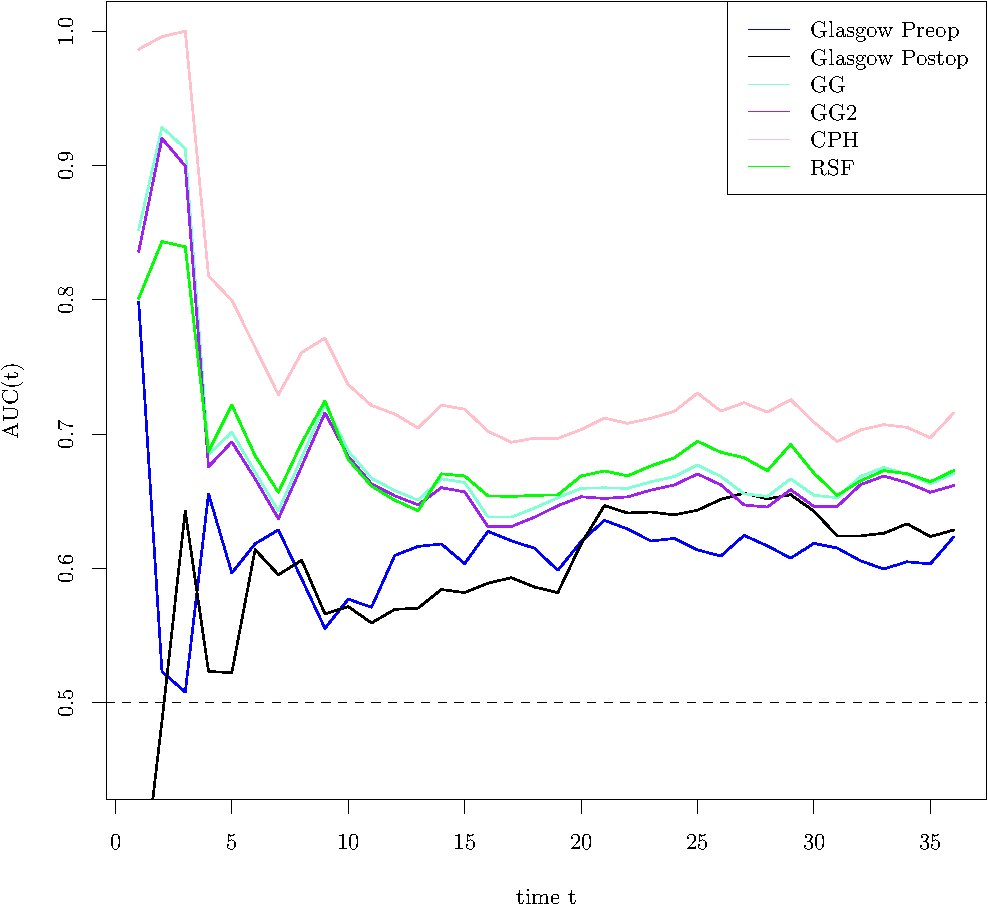
\includegraphics[width=\maxwidth]{figure/05-timeROC-1} 

}



\end{knitrout}

\begin{knitrout}
\definecolor{shadecolor}{rgb}{0.969, 0.969, 0.969}\color{fgcolor}\begin{kframe}
\begin{alltt}
\hlkwd{risksetROC}\hlstd{(data.glasgow}\hlopt{$}\hlstd{Time}\hlopt{/}\hlnum{365.25}\hlopt{*}\hlnum{12}\hlstd{,} \hlkwc{status} \hlstd{= data.glasgow}\hlopt{$}\hlstd{DSD,} \hlkwc{marker} \hlstd{= mskcc_pre.linpred.glasgow,} \hlkwc{predict.time} \hlstd{=} \hlnum{12}\hlstd{)}
\end{alltt}
\end{kframe}

{\centering 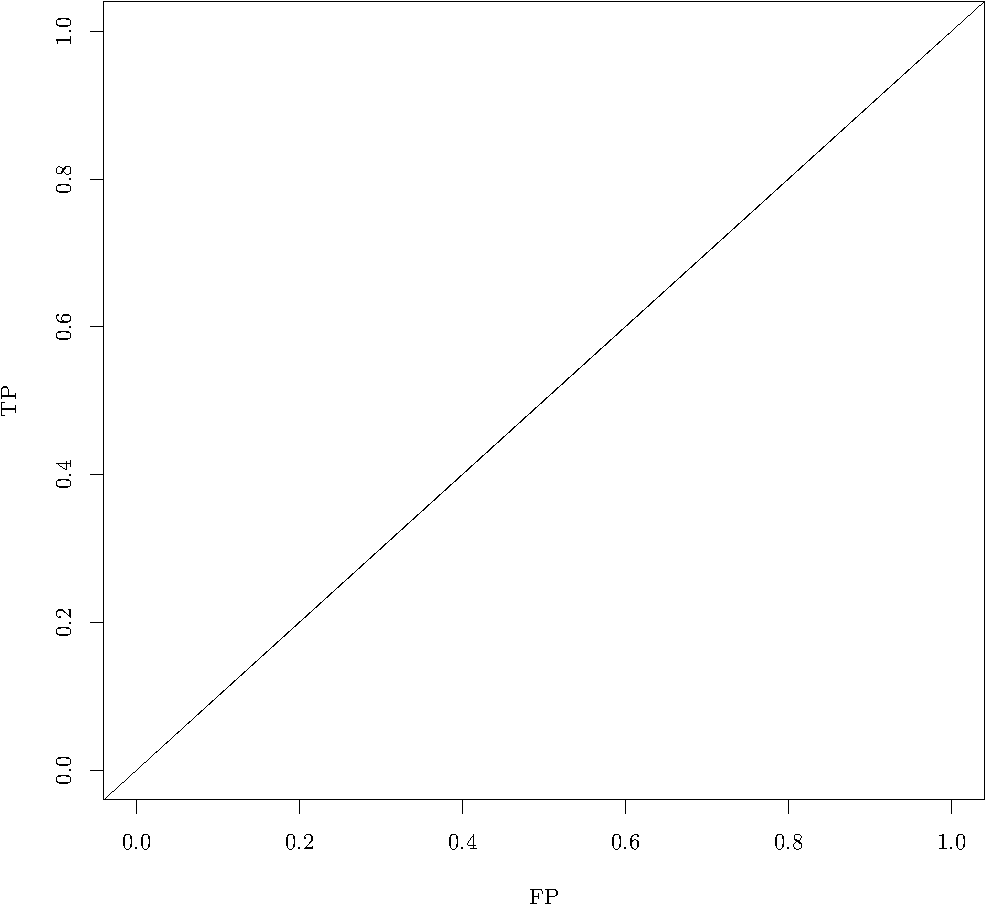
\includegraphics[width=\maxwidth]{figure/05-risksetROC-1} 

}


\begin{kframe}\begin{verbatim}
## $marker
##   [1] -0.09676 -0.08538 -0.07023 -0.07019 -0.06997 -0.06977 -0.06961
##   [8] -0.06958 -0.06955 -0.06950 -0.06947 -0.06928 -0.06917 -0.06916
##  [15] -0.06910 -0.06904 -0.06896 -0.06895 -0.06894 -0.06888 -0.06884
##  [22] -0.06884 -0.06881 -0.06876 -0.06867 -0.06867 -0.06865 -0.06864
##  [29] -0.06860 -0.06860 -0.06859 -0.06859 -0.06856 -0.06856 -0.06855
##  [36] -0.06854 -0.06852 -0.06851 -0.06851 -0.06850 -0.06848 -0.06844
##  [43] -0.06839 -0.06831 -0.06831 -0.06830 -0.06826 -0.06826 -0.06824
##  [50] -0.06823 -0.06823 -0.06823 -0.06823 -0.06823 -0.06822 -0.06821
##  [57] -0.06819 -0.06817 -0.06814 -0.06812 -0.06807 -0.06805 -0.06799
##  [64] -0.06797 -0.06797 -0.06797 -0.06790 -0.06787 -0.06787 -0.06778
##  [71] -0.06775 -0.06772 -0.06755 -0.06752 -0.06752 -0.06750 -0.06748
##  [78] -0.06748 -0.06746 -0.06744 -0.06743 -0.06743 -0.06731 -0.06725
##  [85] -0.06723 -0.06723 -0.06721 -0.06715 -0.06713 -0.06710 -0.06710
##  [92] -0.06709 -0.06704 -0.06704 -0.06703 -0.06703 -0.06703 -0.06703
##  [99] -0.06695 -0.06689 -0.06688 -0.06688 -0.06687 -0.06687 -0.06685
## [106] -0.06680 -0.06675 -0.06670 -0.06669 -0.06662 -0.06658 -0.06512
## [113] -0.06443 -0.06388 -0.06340 -0.06317 -0.06315 -0.06312 -0.06263
## [120] -0.06246 -0.06235 -0.06222 -0.06208 -0.06185
## 
## $TP
##   [1] 1.000000 0.992165 0.984240 0.976194 0.968148 0.960100 0.952051
##   [8] 0.944000 0.935949 0.927898 0.919846 0.911794 0.903741 0.895686
##  [15] 0.887632 0.879577 0.871522 0.863466 0.855409 0.847353 0.839297
##  [22] 0.831240 0.823183 0.815125 0.807068 0.799009 0.790951 0.782893
##  [29] 0.774834 0.766775 0.758716 0.750657 0.742598 0.734539 0.726480
##  [36] 0.718420 0.710361 0.702301 0.694242 0.686182 0.678122 0.670062
##  [43] 0.662002 0.653942 0.645880 0.637819 0.629758 0.621696 0.613634
##  [50] 0.605573 0.597511 0.589449 0.581387 0.573325 0.565263 0.557201
##  [57] 0.549139 0.541077 0.533014 0.524952 0.516889 0.508826 0.500762
##  [64] 0.492698 0.484635 0.476571 0.468507 0.460442 0.452377 0.444312
##  [71] 0.436247 0.428181 0.420115 0.412048 0.403980 0.395912 0.387845
##  [78] 0.379777 0.371709 0.363641 0.355572 0.347504 0.339436 0.331366
##  [85] 0.323296 0.315226 0.307156 0.299086 0.291016 0.282945 0.274874
##  [92] 0.266803 0.258732 0.250660 0.242589 0.234517 0.226446 0.218374
##  [99] 0.210303 0.202230 0.194158 0.186085 0.178012 0.169939 0.161866
## [106] 0.153793 0.145720 0.137646 0.129572 0.121498 0.113423 0.105347
## [113] 0.097260 0.089168 0.081071 0.072970 0.064867 0.056764 0.048661
## [120] 0.040554 0.032445 0.024336 0.016225 0.008114 0.000000 0.000000
## 
## $FP
##   [1] 1.000000 0.991935 0.983871 0.975806 0.967742 0.959677 0.951613
##   [8] 0.943548 0.935484 0.927419 0.919355 0.911290 0.903226 0.895161
##  [15] 0.887097 0.879032 0.870968 0.862903 0.854839 0.846774 0.838710
##  [22] 0.830645 0.822581 0.814516 0.806452 0.798387 0.790323 0.782258
##  [29] 0.774194 0.766129 0.758065 0.750000 0.741935 0.733871 0.725806
##  [36] 0.717742 0.709677 0.701613 0.693548 0.685484 0.677419 0.669355
##  [43] 0.661290 0.653226 0.645161 0.637097 0.629032 0.620968 0.612903
##  [50] 0.604839 0.596774 0.588710 0.580645 0.572581 0.564516 0.556452
##  [57] 0.548387 0.540323 0.532258 0.524194 0.516129 0.508065 0.500000
##  [64] 0.491935 0.483871 0.475806 0.467742 0.459677 0.451613 0.443548
##  [71] 0.435484 0.427419 0.419355 0.411290 0.403226 0.395161 0.387097
##  [78] 0.379032 0.370968 0.362903 0.354839 0.346774 0.338710 0.330645
##  [85] 0.322581 0.314516 0.306452 0.298387 0.290323 0.282258 0.274194
##  [92] 0.266129 0.258065 0.250000 0.241935 0.233871 0.225806 0.217742
##  [99] 0.209677 0.201613 0.193548 0.185484 0.177419 0.169355 0.161290
## [106] 0.153226 0.145161 0.137097 0.129032 0.120968 0.112903 0.104839
## [113] 0.096774 0.088710 0.080645 0.072581 0.064516 0.056452 0.048387
## [120] 0.040323 0.032258 0.024194 0.016129 0.008065 0.000000 0.000000
## 
## $AUC
## [1] 0.5006
\end{verbatim}
\begin{alltt}
\hlkwd{risksetROC}\hlstd{(data.glasgow}\hlopt{$}\hlstd{Time}\hlopt{/}\hlnum{365.25}\hlopt{*}\hlnum{12}\hlstd{,} \hlkwc{status} \hlstd{= data.glasgow}\hlopt{$}\hlstd{DSD,} \hlkwc{marker} \hlstd{= mskcc_post.linpred.glasgow,} \hlkwc{predict.time} \hlstd{=} \hlnum{12}\hlstd{)}
\end{alltt}
\end{kframe}

{\centering 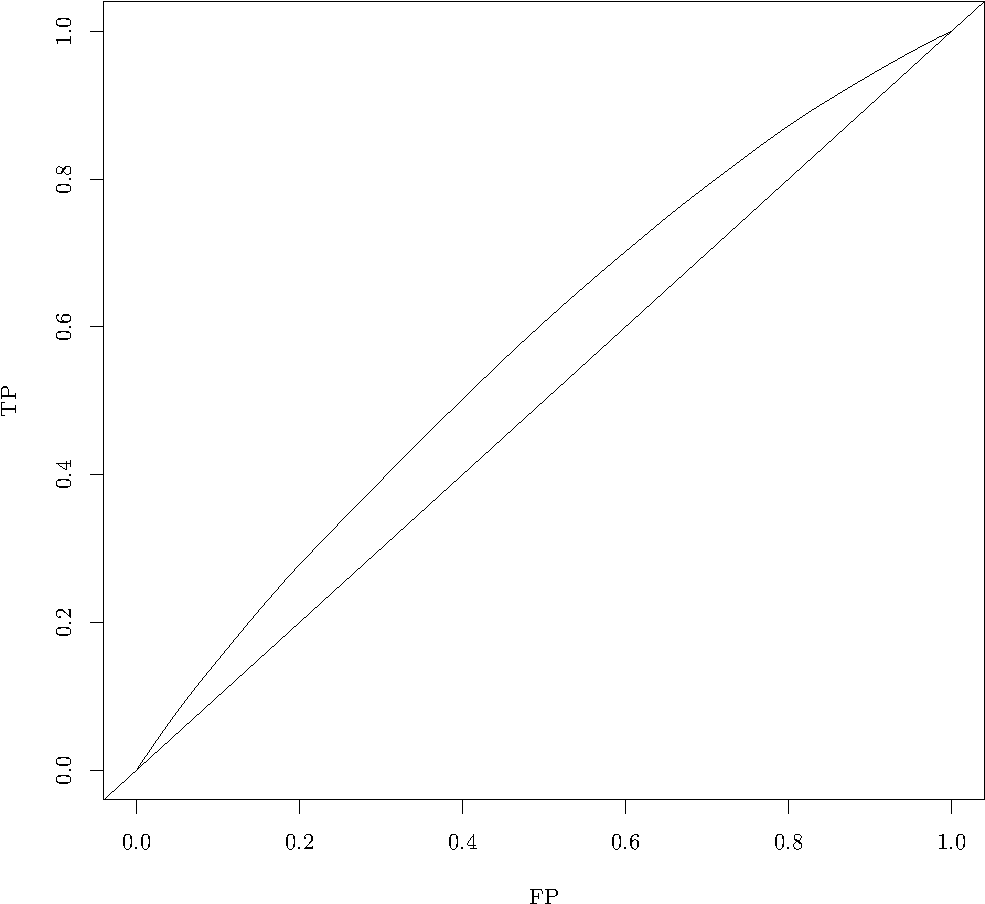
\includegraphics[width=\maxwidth]{figure/05-risksetROC-2} 

}


\begin{kframe}\begin{verbatim}
## $marker
##   [1] 1.734 1.808 1.847 1.877 1.890 1.899 1.901 1.933 1.945 1.953 1.955
##  [12] 1.980 1.984 1.990 2.001 2.009 2.009 2.012 2.016 2.032 2.033 2.086
##  [23] 2.099 2.113 2.136 2.152 2.165 2.182 2.208 2.210 2.224 2.225 2.227
##  [34] 2.229 2.233 2.240 2.245 2.248 2.252 2.259 2.261 2.286 2.295 2.320
##  [45] 2.324 2.331 2.335 2.337 2.341 2.341 2.342 2.347 2.348 2.355 2.379
##  [56] 2.379 2.382 2.384 2.388 2.403 2.404 2.415 2.425 2.426 2.427 2.437
##  [67] 2.451 2.464 2.471 2.474 2.477 2.481 2.485 2.491 2.493 2.495 2.496
##  [78] 2.499 2.515 2.515 2.515 2.521 2.524 2.524 2.527 2.527 2.529 2.531
##  [89] 2.533 2.538 2.541 2.545 2.548 2.548 2.555 2.558 2.564 2.567 2.572
## [100] 2.572 2.604 2.650 2.656 2.656 2.669 2.679 2.685 2.710 2.711 2.714
## [111] 2.717 2.718 2.721 2.726 2.742 2.766 2.779 2.806 2.850 2.860 2.883
## [122] 2.884 2.895 2.938
## 
## $TP
##   [1] 1.00000 0.99594 0.99156 0.98701 0.98232 0.97757 0.97278 0.96798
##   [9] 0.96302 0.95801 0.95295 0.94788 0.94269 0.93747 0.93222 0.92691
##  [17] 0.92156 0.91621 0.91085 0.90546 0.89999 0.89451 0.88873 0.88288
##  [25] 0.87695 0.87087 0.86471 0.85845 0.85209 0.84557 0.83903 0.83240
##  [33] 0.82576 0.81911 0.81244 0.80575 0.79901 0.79224 0.78544 0.77862
##  [41] 0.77175 0.76487 0.75782 0.75070 0.74340 0.73607 0.72869 0.72127
##  [49] 0.71385 0.70640 0.69894 0.69148 0.68398 0.67648 0.66892 0.66118
##  [57] 0.65343 0.64566 0.63788 0.63007 0.62214 0.61419 0.60616 0.59806
##  [65] 0.58994 0.58181 0.57361 0.56529 0.55686 0.54837 0.53986 0.53132
##  [73] 0.52275 0.51413 0.50547 0.49679 0.48810 0.47939 0.47066 0.46179
##  [81] 0.45292 0.44405 0.43513 0.42618 0.41723 0.40825 0.39927 0.39027
##  [89] 0.38126 0.37223 0.36315 0.35404 0.34490 0.33573 0.32657 0.31734
##  [97] 0.30808 0.29875 0.28940 0.28001 0.27062 0.26092 0.25077 0.24056
## [105] 0.23035 0.22000 0.20955 0.19903 0.18825 0.17745 0.16663 0.15577
## [113] 0.14490 0.13400 0.12305 0.11191 0.10051 0.08895 0.07709 0.06469
## [121] 0.05217 0.03935 0.02651 0.01354 0.00000 0.00000
## 
## $FP
##   [1] 1.000000 0.991935 0.983871 0.975806 0.967742 0.959677 0.951613
##   [8] 0.943548 0.935484 0.927419 0.919355 0.911290 0.903226 0.895161
##  [15] 0.887097 0.879032 0.870968 0.862903 0.854839 0.846774 0.838710
##  [22] 0.830645 0.822581 0.814516 0.806452 0.798387 0.790323 0.782258
##  [29] 0.774194 0.766129 0.758065 0.750000 0.741935 0.733871 0.725806
##  [36] 0.717742 0.709677 0.701613 0.693548 0.685484 0.677419 0.669355
##  [43] 0.661290 0.653226 0.645161 0.637097 0.629032 0.620968 0.612903
##  [50] 0.604839 0.596774 0.588710 0.580645 0.572581 0.564516 0.556452
##  [57] 0.548387 0.540323 0.532258 0.524194 0.516129 0.508065 0.500000
##  [64] 0.491935 0.483871 0.475806 0.467742 0.459677 0.451613 0.443548
##  [71] 0.435484 0.427419 0.419355 0.411290 0.403226 0.395161 0.387097
##  [78] 0.379032 0.370968 0.362903 0.354839 0.346774 0.338710 0.330645
##  [85] 0.322581 0.314516 0.306452 0.298387 0.290323 0.282258 0.274194
##  [92] 0.266129 0.258065 0.250000 0.241935 0.233871 0.225806 0.217742
##  [99] 0.209677 0.201613 0.193548 0.185484 0.177419 0.169355 0.161290
## [106] 0.153226 0.145161 0.137097 0.129032 0.120968 0.112903 0.104839
## [113] 0.096774 0.088710 0.080645 0.072581 0.064516 0.056452 0.048387
## [120] 0.040323 0.032258 0.024194 0.016129 0.008065 0.000000 0.000000
## 
## $AUC
## [1] 0.5743
\end{verbatim}
\begin{alltt}
\hlkwd{risksetROC}\hlstd{(data.glasgow}\hlopt{$}\hlstd{Time}\hlopt{/}\hlnum{365.25}\hlopt{*}\hlnum{12}\hlstd{,} \hlkwc{status} \hlstd{= data.glasgow}\hlopt{$}\hlstd{DSD,} \hlkwc{marker} \hlstd{= gg.linpred.glasgow,} \hlkwc{predict.time} \hlstd{=} \hlnum{12}\hlstd{)}
\end{alltt}
\end{kframe}

{\centering 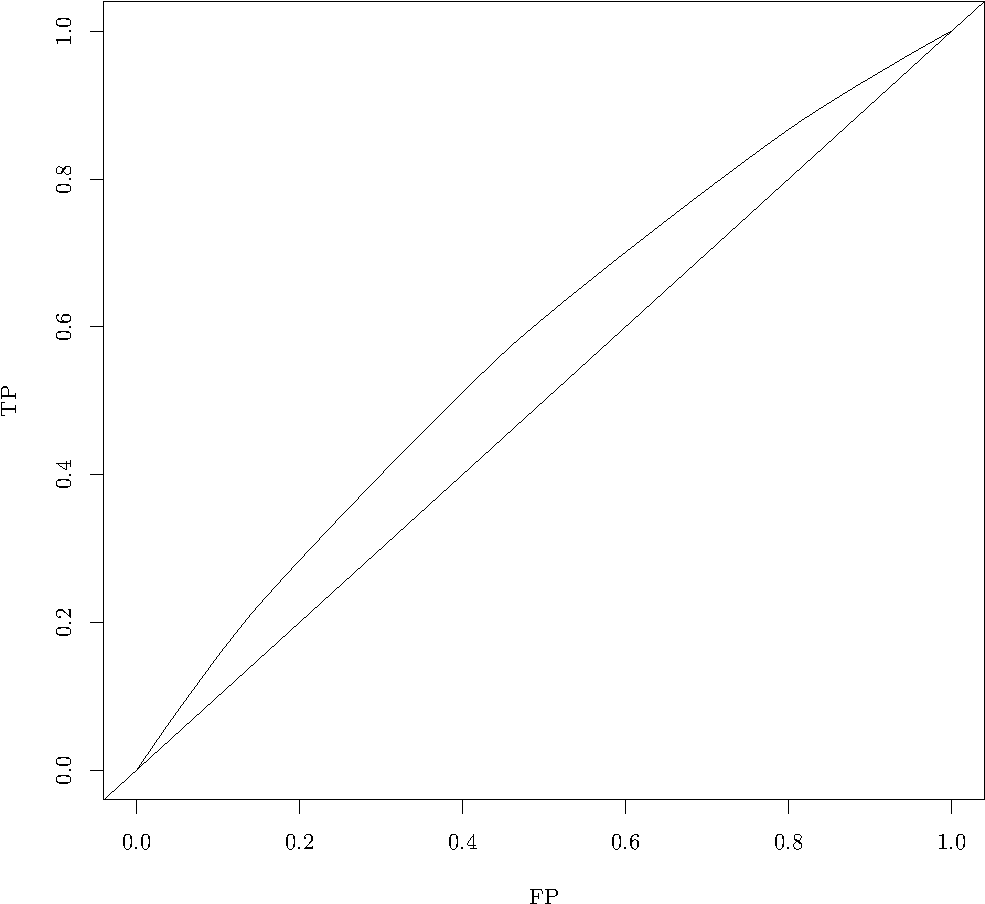
\includegraphics[width=\maxwidth]{figure/05-risksetROC-3} 

}


\begin{kframe}\begin{verbatim}
## $marker
##   [1] -0.467684 -0.371761 -0.346182 -0.346182 -0.346182 -0.339787 -0.339787
##   [8] -0.307812 -0.307812 -0.307812 -0.307812 -0.307812 -0.307812 -0.307812
##  [15] -0.275838 -0.275838 -0.263048 -0.243864 -0.243864 -0.243864 -0.243864
##  [22] -0.211889 -0.206711 -0.147941 -0.142762 -0.142762 -0.110788 -0.097998
##  [29] -0.095923 -0.095923 -0.083133 -0.078814 -0.078814 -0.078814 -0.078814
##  [36] -0.072419 -0.063949 -0.063949 -0.046839 -0.046839 -0.046839 -0.046839
##  [43] -0.046839 -0.040444 -0.034049 -0.031974 -0.031974 -0.031974 -0.031974
##  [50] -0.025580 -0.014865 -0.014865 -0.014865 -0.012790  0.000000  0.000000
##  [57]  0.000000  0.000000  0.006395  0.031974  0.031974  0.031974  0.031974
##  [64]  0.049084  0.049084  0.081058  0.081058  0.140687  0.153779  0.158957
##  [71]  0.184235  0.184235  0.190630  0.197024  0.197024  0.197024  0.203721
##  [78]  0.222604  0.222906  0.222906  0.228999  0.228999  0.228999  0.228999
##  [85]  0.248184  0.254880  0.254880  0.260973  0.260973  0.260973  0.260973
##  [92]  0.260973  0.260973  0.260973  0.269745  0.286855  0.286855  0.286855
##  [99]  0.286855  0.288930  0.292948  0.318829  0.324922  0.324922  0.324922
## [106]  0.350803  0.388871  0.429617  0.452820  0.466770  0.466770  0.492349
## [113]  0.524324  0.530718  0.530718  0.530718  0.530718  0.549903  0.562693
## [120]  0.562693  0.594667  0.594667  0.594667  0.594667
## 
## $TP
##   [1] 1.00000 0.99552 0.99060 0.98554 0.98049 0.97543 0.97035 0.96526
##   [9] 0.96001 0.95476 0.94950 0.94425 0.93900 0.93375 0.92849 0.92307
##  [17] 0.91765 0.91216 0.90656 0.90096 0.89536 0.88976 0.88398 0.87817
##  [25] 0.87201 0.86581 0.85962 0.85322 0.84674 0.84025 0.83376 0.82718
##  [33] 0.82058 0.81398 0.80737 0.80077 0.79412 0.78742 0.78072 0.77390
##  [41] 0.76708 0.76026 0.75344 0.74662 0.73976 0.73286 0.72594 0.71902
##  [49] 0.71209 0.70517 0.69821 0.69117 0.68413 0.67709 0.67004 0.66289
##  [57] 0.65574 0.64860 0.64145 0.63426 0.62689 0.61951 0.61213 0.60475
##  [65] 0.59725 0.58974 0.58199 0.57425 0.56602 0.55769 0.54931 0.54072
##  [73] 0.53213 0.52348 0.51478 0.50608 0.49738 0.48862 0.47969 0.47076
##  [81] 0.46183 0.45285 0.44387 0.43488 0.42590 0.41674 0.40752 0.39830
##  [89] 0.38902 0.37975 0.37047 0.36120 0.35192 0.34264 0.33337 0.32401
##  [97] 0.31449 0.30497 0.29545 0.28593 0.27639 0.26682 0.25699 0.24710
## [105] 0.23721 0.22732 0.21718 0.20663 0.19565 0.18442 0.17302 0.16162
## [113] 0.14993 0.13786 0.12572 0.11357 0.10142 0.08927 0.07689 0.06434
## [121] 0.05180 0.03885 0.02590 0.01295 0.00000 0.00000
## 
## $FP
##   [1] 1.000000 0.991935 0.983871 0.975806 0.967742 0.959677 0.951613
##   [8] 0.943548 0.935484 0.927419 0.919355 0.911290 0.903226 0.895161
##  [15] 0.887097 0.879032 0.870968 0.862903 0.854839 0.846774 0.838710
##  [22] 0.830645 0.822581 0.814516 0.806452 0.798387 0.790323 0.782258
##  [29] 0.774194 0.766129 0.758065 0.750000 0.741935 0.733871 0.725806
##  [36] 0.717742 0.709677 0.701613 0.693548 0.685484 0.677419 0.669355
##  [43] 0.661290 0.653226 0.645161 0.637097 0.629032 0.620968 0.612903
##  [50] 0.604839 0.596774 0.588710 0.580645 0.572581 0.564516 0.556452
##  [57] 0.548387 0.540323 0.532258 0.524194 0.516129 0.508065 0.500000
##  [64] 0.491935 0.483871 0.475806 0.467742 0.459677 0.451613 0.443548
##  [71] 0.435484 0.427419 0.419355 0.411290 0.403226 0.395161 0.387097
##  [78] 0.379032 0.370968 0.362903 0.354839 0.346774 0.338710 0.330645
##  [85] 0.322581 0.314516 0.306452 0.298387 0.290323 0.282258 0.274194
##  [92] 0.266129 0.258065 0.250000 0.241935 0.233871 0.225806 0.217742
##  [99] 0.209677 0.201613 0.193548 0.185484 0.177419 0.169355 0.161290
## [106] 0.153226 0.145161 0.137097 0.129032 0.120968 0.112903 0.104839
## [113] 0.096774 0.088710 0.080645 0.072581 0.064516 0.056452 0.048387
## [120] 0.040323 0.032258 0.024194 0.016129 0.008065 0.000000 0.000000
## 
## $AUC
## [1] 0.5762
\end{verbatim}
\begin{alltt}
\hlkwd{risksetROC}\hlstd{(data.glasgow}\hlopt{$}\hlstd{Time}\hlopt{/}\hlnum{365.25}\hlopt{*}\hlnum{12}\hlstd{,} \hlkwc{status} \hlstd{= data.glasgow}\hlopt{$}\hlstd{DSD,} \hlkwc{marker} \hlstd{= gg2.linpred.glasgow,} \hlkwc{predict.time} \hlstd{=} \hlnum{12}\hlstd{)}
\end{alltt}
\end{kframe}

{\centering 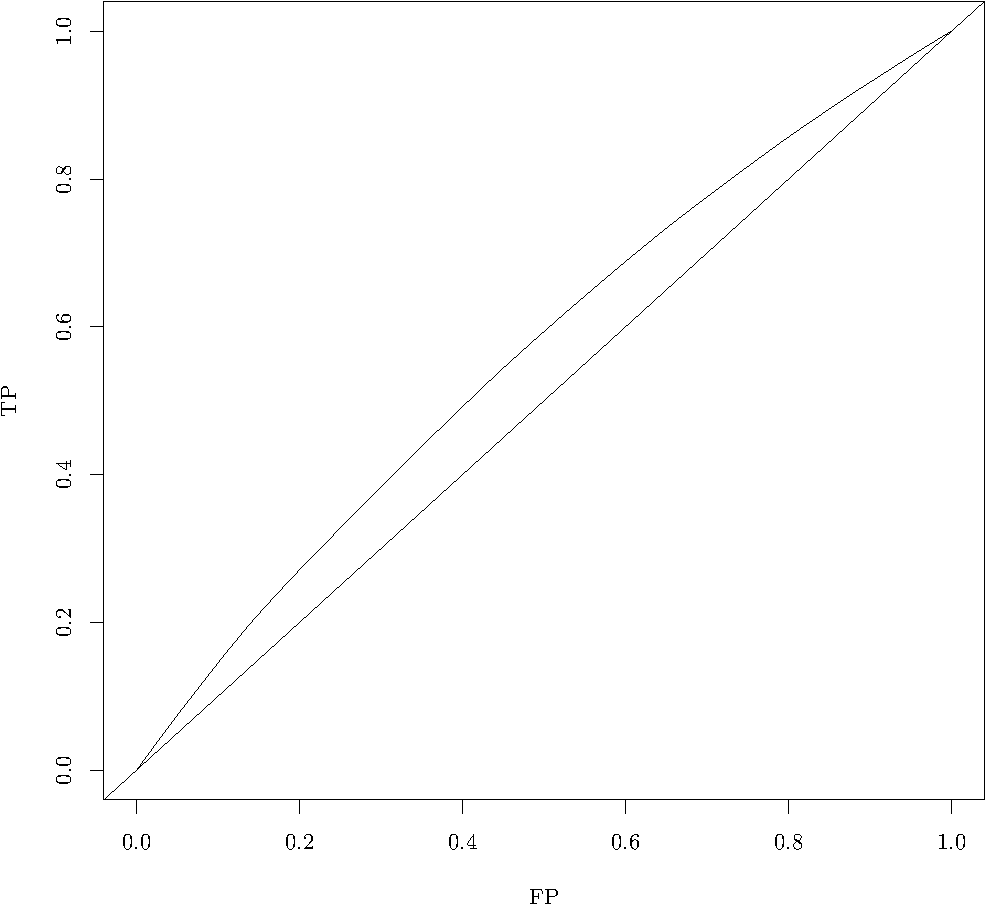
\includegraphics[width=\maxwidth]{figure/05-risksetROC-4} 

}


\begin{kframe}\begin{verbatim}
## $marker
##   [1] -0.450187 -0.365769 -0.343257 -0.343257 -0.343257 -0.337630 -0.337630
##   [8] -0.309490 -0.309490 -0.309490 -0.309490 -0.309490 -0.309490 -0.309490
##  [15] -0.292441 -0.281351 -0.281351 -0.270095 -0.253212 -0.253212 -0.253212
##  [22] -0.253212 -0.236163 -0.236163 -0.225072 -0.208024 -0.196768 -0.179884
##  [29] -0.179884 -0.179884 -0.179884 -0.174256 -0.168794 -0.151745 -0.151745
##  [36] -0.151745 -0.151745 -0.151745 -0.146117 -0.140489 -0.123606 -0.123606
##  [43] -0.123606 -0.084418 -0.084418 -0.073162 -0.067327 -0.067327 -0.056279
##  [50] -0.056279 -0.039188 -0.039188 -0.028139 -0.028139 -0.028139 -0.028139
##  [57] -0.022511 -0.011256  0.000000  0.000000  0.000000  0.000000  0.005628
##  [64]  0.018497  0.028139  0.028139  0.028139  0.028139  0.057892  0.074776
##  [71]  0.074776  0.085866  0.090211  0.090211  0.095839  0.101467  0.101467
##  [78]  0.101467  0.102915  0.102915  0.123813  0.123978  0.129606  0.129606
##  [85]  0.129606  0.129606  0.131055  0.131055  0.131055  0.131055  0.146490
##  [92]  0.157745  0.157745  0.157745  0.157745  0.157745  0.157745  0.157745
##  [99]  0.159194  0.185885  0.187333  0.214024  0.214024  0.214024  0.226521
## [106]  0.243405  0.270302  0.326581  0.327988  0.327988  0.350499  0.367217
## [113]  0.378638  0.384266  0.384266  0.384266  0.384266  0.401150  0.412406
## [120]  0.412406  0.440545  0.440545  0.440545  0.440545
## 
## $TP
##   [1] 1.00000 0.99504 0.98963 0.98411 0.97858 0.97306 0.96750 0.96194
##   [9] 0.95623 0.95051 0.94480 0.93908 0.93337 0.92765 0.92194 0.91612
##  [17] 0.91025 0.90437 0.89842 0.89238 0.88633 0.88029 0.87424 0.86809
##  [25] 0.86194 0.85572 0.84940 0.84300 0.83649 0.82999 0.82348 0.81698
##  [33] 0.81043 0.80385 0.79716 0.79047 0.78378 0.77709 0.77040 0.76367
##  [41] 0.75690 0.75002 0.74313 0.73625 0.72909 0.72194 0.71470 0.70742
##  [49] 0.70014 0.69277 0.68541 0.67792 0.67044 0.66286 0.65529 0.64772
##  [57] 0.64015 0.63253 0.62483 0.61704 0.60926 0.60147 0.59368 0.58585
##  [65] 0.57791 0.56990 0.56189 0.55388 0.54587 0.53762 0.52923 0.52083
##  [73] 0.51235 0.50382 0.49530 0.48673 0.47811 0.46949 0.46087 0.45224
##  [81] 0.44361 0.43479 0.42597 0.41711 0.40824 0.39938 0.39051 0.38163
##  [89] 0.37275 0.36388 0.35500 0.34598 0.33686 0.32774 0.31862 0.30950
##  [97] 0.30039 0.29127 0.28215 0.27302 0.26364 0.25424 0.24460 0.23495
## [105] 0.22530 0.21554 0.20560 0.19540 0.18460 0.17379 0.16298 0.15192
## [113] 0.14068 0.12930 0.11787 0.10643 0.09499 0.08356 0.07192 0.06016
## [121] 0.04840 0.03630 0.02420 0.01210 0.00000 0.00000
## 
## $FP
##   [1] 1.000000 0.991935 0.983871 0.975806 0.967742 0.959677 0.951613
##   [8] 0.943548 0.935484 0.927419 0.919355 0.911290 0.903226 0.895161
##  [15] 0.887097 0.879032 0.870968 0.862903 0.854839 0.846774 0.838710
##  [22] 0.830645 0.822581 0.814516 0.806452 0.798387 0.790323 0.782258
##  [29] 0.774194 0.766129 0.758065 0.750000 0.741935 0.733871 0.725806
##  [36] 0.717742 0.709677 0.701613 0.693548 0.685484 0.677419 0.669355
##  [43] 0.661290 0.653226 0.645161 0.637097 0.629032 0.620968 0.612903
##  [50] 0.604839 0.596774 0.588710 0.580645 0.572581 0.564516 0.556452
##  [57] 0.548387 0.540323 0.532258 0.524194 0.516129 0.508065 0.500000
##  [64] 0.491935 0.483871 0.475806 0.467742 0.459677 0.451613 0.443548
##  [71] 0.435484 0.427419 0.419355 0.411290 0.403226 0.395161 0.387097
##  [78] 0.379032 0.370968 0.362903 0.354839 0.346774 0.338710 0.330645
##  [85] 0.322581 0.314516 0.306452 0.298387 0.290323 0.282258 0.274194
##  [92] 0.266129 0.258065 0.250000 0.241935 0.233871 0.225806 0.217742
##  [99] 0.209677 0.201613 0.193548 0.185484 0.177419 0.169355 0.161290
## [106] 0.153226 0.145161 0.137097 0.129032 0.120968 0.112903 0.104839
## [113] 0.096774 0.088710 0.080645 0.072581 0.064516 0.056452 0.048387
## [120] 0.040323 0.032258 0.024194 0.016129 0.008065 0.000000 0.000000
## 
## $AUC
## [1] 0.5645
\end{verbatim}
\begin{alltt}
\hlkwd{risksetROC}\hlstd{(data.glasgow}\hlopt{$}\hlstd{Time}\hlopt{/}\hlnum{365.25}\hlopt{*}\hlnum{12}\hlstd{,} \hlkwc{status} \hlstd{= data.glasgow}\hlopt{$}\hlstd{DSD,} \hlkwc{marker} \hlstd{= cph.linpred.glasgow,} \hlkwc{predict.time} \hlstd{=} \hlnum{12}\hlstd{)}
\end{alltt}
\end{kframe}

{\centering 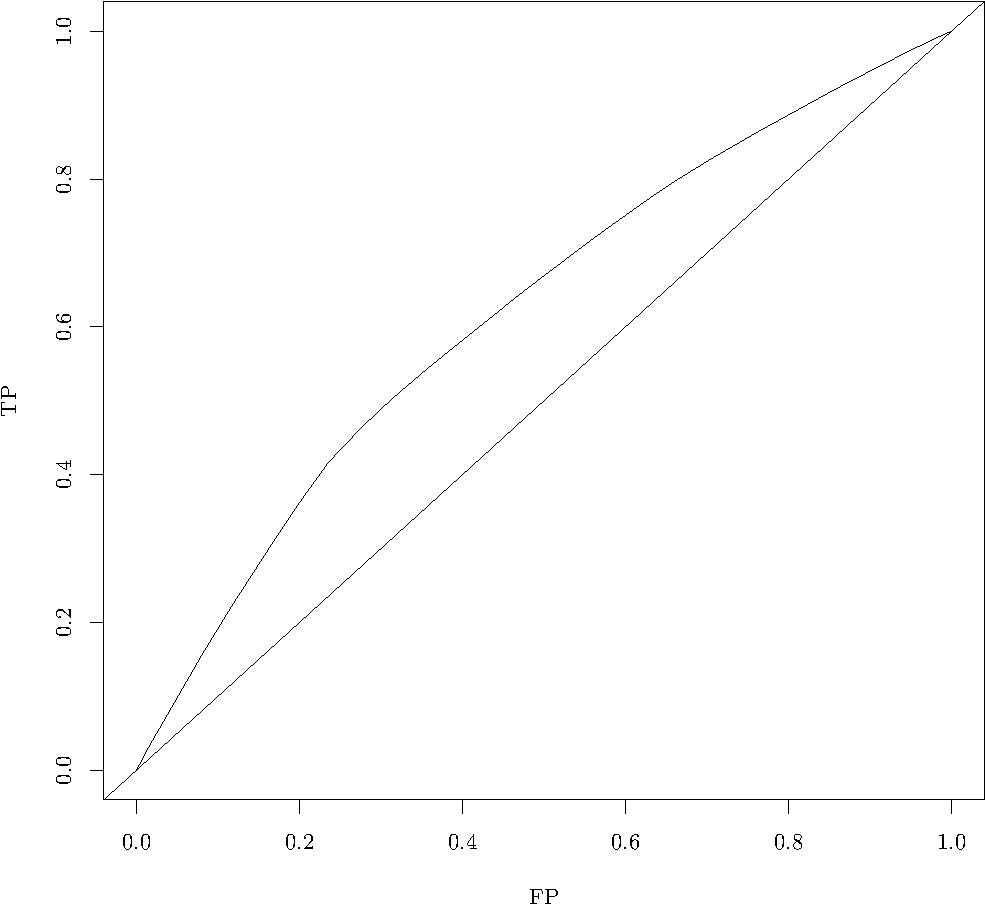
\includegraphics[width=\maxwidth]{figure/05-risksetROC-5} 

}


\begin{kframe}\begin{verbatim}
## $marker
##   [1] -0.34542 -0.20725 -0.20725 -0.17962 -0.13817 -0.13817 -0.13817
##   [8] -0.08290 -0.08290 -0.08290 -0.06908 -0.06908 -0.06908 -0.06908
##  [15] -0.06908 -0.06908 -0.05527 -0.02763  0.00000  0.00000  0.00000
##  [22]  0.00000  0.00000  0.00000  0.00000  0.00000  0.00000  0.00000
##  [29]  0.00000  0.01382  0.06908  0.06908  0.06908  0.06908  0.06908
##  [36]  0.06908  0.09672  0.13540  0.13817  0.13817  0.13817  0.13817
##  [43]  0.20725  0.27357  0.27357  0.30397  0.31502  0.31502  0.32883
##  [50]  0.34265  0.34265  0.34265  0.34265  0.34542  0.37028  0.39792
##  [57]  0.41173  0.41173  0.41173  0.41173  0.41173  0.41173  0.41173
##  [64]  0.41173  0.42555  0.45318  0.48082  0.48082  0.48082  0.48082
##  [71]  0.48082  0.48082  0.48082  0.48082  0.48082  0.48082  0.48082
##  [78]  0.48082  0.49463  0.50845  0.54990  0.54990  0.54990  0.54990
##  [85]  0.56413  0.60558  0.61898  0.61898  0.61898  0.68807  0.68807
##  [92]  0.75715  0.75715  0.75715  0.89532  0.90678  0.90678  0.90678
##  [99]  0.90955  0.96205  0.97863  1.00350  1.03113  1.04495  1.04495
## [106]  1.04495  1.04495  1.04495  1.04495  1.08640  1.11403  1.11403
## [113]  1.11403  1.11403  1.18311  1.18311  1.18311  1.18311  1.18311
## [120]  1.18311  1.18311  1.18311  1.25220  1.32128
## 
## $TP
##   [1] 1.00000 0.99669 0.99289 0.98908 0.98518 0.98110 0.97703 0.97295
##   [9] 0.96865 0.96434 0.96004 0.95567 0.95130 0.94694 0.94257 0.93821
##  [17] 0.93384 0.92942 0.92487 0.92019 0.91551 0.91083 0.90615 0.90148
##  [25] 0.89680 0.89212 0.88744 0.88277 0.87809 0.87341 0.86867 0.86365
##  [33] 0.85864 0.85363 0.84862 0.84361 0.83859 0.83344 0.82808 0.82271
##  [41] 0.81734 0.81197 0.80660 0.80085 0.79470 0.78855 0.78221 0.77580
##  [49] 0.76939 0.76289 0.75630 0.74971 0.74312 0.73653 0.72992 0.72315
##  [57] 0.71618 0.70912 0.70206 0.69500 0.68794 0.68088 0.67382 0.66676
##  [65] 0.65970 0.65254 0.64518 0.63761 0.63005 0.62248 0.61492 0.60735
##  [73] 0.59978 0.59222 0.58465 0.57709 0.56952 0.56195 0.55439 0.54672
##  [81] 0.53894 0.53083 0.52273 0.51462 0.50651 0.49829 0.48972 0.48103
##  [89] 0.47234 0.46366 0.45435 0.44504 0.43507 0.42509 0.41512 0.40367
##  [97] 0.39208 0.38050 0.36892 0.35730 0.34506 0.33261 0.31985 0.30673
## [105] 0.29343 0.28013 0.26683 0.25353 0.24023 0.22693 0.21307 0.19882
## [113] 0.18457 0.17031 0.15606 0.14079 0.12552 0.11025 0.09498 0.07971
## [121] 0.06444 0.04917 0.03390 0.01753 0.00000 0.00000
## 
## $FP
##   [1] 1.000000 0.991935 0.983871 0.975806 0.967742 0.959677 0.951613
##   [8] 0.943548 0.935484 0.927419 0.919355 0.911290 0.903226 0.895161
##  [15] 0.887097 0.879032 0.870968 0.862903 0.854839 0.846774 0.838710
##  [22] 0.830645 0.822581 0.814516 0.806452 0.798387 0.790323 0.782258
##  [29] 0.774194 0.766129 0.758065 0.750000 0.741935 0.733871 0.725806
##  [36] 0.717742 0.709677 0.701613 0.693548 0.685484 0.677419 0.669355
##  [43] 0.661290 0.653226 0.645161 0.637097 0.629032 0.620968 0.612903
##  [50] 0.604839 0.596774 0.588710 0.580645 0.572581 0.564516 0.556452
##  [57] 0.548387 0.540323 0.532258 0.524194 0.516129 0.508065 0.500000
##  [64] 0.491935 0.483871 0.475806 0.467742 0.459677 0.451613 0.443548
##  [71] 0.435484 0.427419 0.419355 0.411290 0.403226 0.395161 0.387097
##  [78] 0.379032 0.370968 0.362903 0.354839 0.346774 0.338710 0.330645
##  [85] 0.322581 0.314516 0.306452 0.298387 0.290323 0.282258 0.274194
##  [92] 0.266129 0.258065 0.250000 0.241935 0.233871 0.225806 0.217742
##  [99] 0.209677 0.201613 0.193548 0.185484 0.177419 0.169355 0.161290
## [106] 0.153226 0.145161 0.137097 0.129032 0.120968 0.112903 0.104839
## [113] 0.096774 0.088710 0.080645 0.072581 0.064516 0.056452 0.048387
## [120] 0.040323 0.032258 0.024194 0.016129 0.008065 0.000000 0.000000
## 
## $AUC
## [1] 0.6232
\end{verbatim}
\begin{alltt}
\hlkwd{risksetAUC}\hlstd{(data.glasgow}\hlopt{$}\hlstd{Time}\hlopt{/}\hlnum{365.25}\hlopt{*}\hlnum{12}\hlstd{,} \hlkwc{status} \hlstd{= data.glasgow}\hlopt{$}\hlstd{DSD,} \hlkwc{marker} \hlstd{= mskcc_pre.linpred.glasgow,} \hlkwc{tmax} \hlstd{=} \hlnum{36}\hlstd{)}
\end{alltt}
\end{kframe}

{\centering 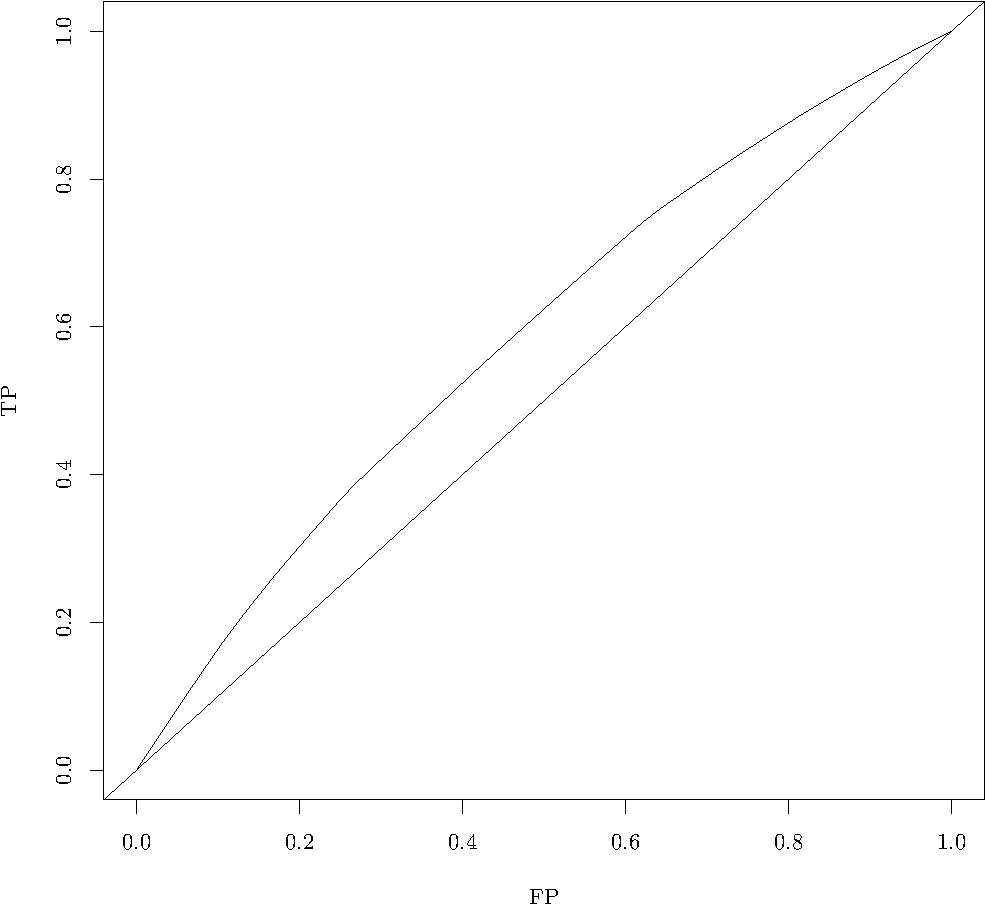
\includegraphics[width=\maxwidth]{figure/05-risksetROC-6} 

}


\begin{kframe}\begin{verbatim}
## $utimes
##   [1]   0.80   1.63   2.50   3.00   3.40   3.73   3.83   3.90   4.47   4.57
##  [11]   4.67   4.73   4.83   4.87   5.00   5.30   5.77   5.83   5.87   6.00
##  [21]   6.10   6.27   6.30   6.67   6.93   7.00   7.10   7.66   7.67   7.73
##  [31]   8.00   8.17   8.33   8.43   8.47   8.77   8.80   9.00   9.03   9.30
##  [41]   9.40   9.83  10.13  10.27  10.40  10.50  11.07  11.30  11.33  11.50
##  [51]  11.60  11.90  12.33  12.47  12.97  13.00  13.03  13.10  13.30  13.43
##  [61]  13.50  13.57  13.70  13.93  14.00  14.80  15.37  15.40  15.57  16.00
##  [71]  16.17  16.33  16.47  16.77  16.95  17.00  17.07  17.57  17.83  18.03
##  [81]  18.17  18.40  18.50  18.57  18.93  19.10  19.50  19.63  19.80  20.00
##  [91]  20.07  20.43  20.67  20.90  21.53  21.80  22.00  22.60  23.07  23.10
## [101]  23.17  24.00  24.37  24.70  25.00  25.67  25.83  26.33  26.40  26.50
## [111]  26.60  26.70  27.53  28.13  28.33  28.53  29.03  29.10  29.27  29.60
## [121]  29.67  30.07  30.97  31.00  31.53  32.00  33.00  33.10  33.40  33.47
## [131]  34.37  35.10  35.97  36.23  36.30  36.67  37.00  38.00  39.60  41.23
## [141]  43.07  45.37  46.67  47.43  47.73  48.00  49.00  51.00  54.90  59.00
## [151]  63.13  65.00  67.00  70.00  77.00  85.00  85.80  90.33  93.00  94.77
## [161] 116.00
## 
## $St
##   [1] 0.99476 0.98930 0.98383 0.97834 0.97284 0.96734 0.96185 0.95086
##   [9] 0.93986 0.93437 0.92887 0.92337 0.91788 0.90689 0.89589 0.89040
##  [17] 0.88490 0.87940 0.87391 0.86841 0.86291 0.85742 0.85192 0.84643
##  [25] 0.84093 0.83543 0.82994 0.82444 0.81894 0.81345 0.80246 0.79696
##  [33] 0.79146 0.78597 0.78047 0.77497 0.76948 0.76398 0.75845 0.75291
##  [41] 0.74737 0.74184 0.73630 0.73077 0.72523 0.71969 0.71416 0.70862
##  [49] 0.70308 0.69755 0.69201 0.68648 0.68094 0.67540 0.66987 0.66433
##  [57] 0.65880 0.65326 0.64772 0.64219 0.63665 0.63112 0.62558 0.62004
##  [65] 0.61451 0.60892 0.60333 0.59775 0.59216 0.58658 0.58099 0.57540
##  [73] 0.56982 0.56423 0.55864 0.55306 0.54747 0.54188 0.53630 0.53071
##  [81] 0.52512 0.51954 0.51395 0.50837 0.50278 0.49719 0.49161 0.48602
##  [89] 0.48043 0.46926 0.46367 0.45809 0.45250 0.44691 0.44133 0.43574
##  [97] 0.43016 0.42457 0.41898 0.41340 0.40781 0.39664 0.39105 0.38546
## [105] 0.37429 0.36870 0.36312 0.35753 0.35195 0.34636 0.34077 0.33519
## [113] 0.32960 0.32401 0.31843 0.31284 0.30725 0.30167 0.29608 0.29049
## [121] 0.28491 0.27932 0.27374 0.26815 0.26256 0.25698 0.25139 0.24580
## [129] 0.24022 0.23463 0.22904 0.22332 0.21759 0.21187 0.20614 0.20041
## [137] 0.19469 0.18289 0.17679 0.17048 0.16416 0.15760 0.15103 0.14446
## [145] 0.13790 0.13133 0.12442 0.11751 0.10967 0.10184 0.09401 0.08617
## [153] 0.07834 0.07050 0.06169 0.05141 0.04113 0.03085 0.02056 0.01028
## [161] 0.00000
## 
## $AUC
##   [1] 0.4989 0.5018 0.5007 0.4988 0.4998 0.5010 0.4988 0.4968 0.4984 0.4989
##  [11] 0.5023 0.4989 0.5000 0.5035 0.4984 0.4978 0.5021 0.5003 0.4981 0.4998
##  [21] 0.5003 0.4976 0.5006 0.4977 0.5014 0.5022 0.4994 0.5014 0.5030 0.4995
##  [31] 0.5041 0.5014 0.5013 0.5028 0.5001 0.5008 0.4985 0.4997 0.5009 0.4975
##  [41] 0.4997 0.4981 0.5004 0.4986 0.5012 0.5020 0.4969 0.4983 0.4993 0.5005
##  [51] 0.4980 0.4970 0.5000 0.4969 0.5020 0.4979 0.5014 0.4972 0.5006 0.4986
##  [61] 0.4986 0.4990 0.5009 0.5036 0.5006 0.5039 0.4983 0.4976 0.4965 0.4982
##  [71] 0.5001 0.5017 0.5012 0.5039 0.4965 0.4993 0.4994 0.5034 0.4995 0.5002
##  [81] 0.5013 0.5050 0.5021 0.4999 0.4990 0.5013 0.4980 0.4956 0.4959 0.5007
##  [91] 0.4955 0.5002 0.4966 0.4984 0.5020 0.5026 0.4970 0.5066 0.4956 0.4959
## [101] 0.5044 0.5087 0.5064 0.4963 0.4999 0.5062 0.4963 0.4960 0.4972 0.4960
## [111] 0.5002 0.4997 0.5052 0.4962 0.5086 0.5018 0.4949 0.4941 0.4986 0.5034
## [121] 0.5034 0.5088 0.4983 0.4958 0.5012 0.5074 0.5017 0.4949 0.4933 0.5127
## [131] 0.4955 0.4911 0.4956 0.5107 0.5063 0.4927 0.4910 0.4962 0.4960 0.4900
## [141] 0.4942 0.4897 0.4932 0.5232 0.5198 0.4847 0.5216 0.4930 0.5204 0.4821
## [151] 0.4758 0.5357 0.4924 0.4517 0.4380 0.4171 0.4504 0.6255 0.5000 0.7500
## [161] 0.0000
## 
## $Cindex
## [1] 0.5
\end{verbatim}
\begin{alltt}
\hlkwd{risksetAUC}\hlstd{(data.glasgow}\hlopt{$}\hlstd{Time}\hlopt{/}\hlnum{365.25}\hlopt{*}\hlnum{12}\hlstd{,} \hlkwc{status} \hlstd{= data.glasgow}\hlopt{$}\hlstd{DSD,} \hlkwc{marker} \hlstd{= mskcc_post.linpred.glasgow,} \hlkwc{tmax} \hlstd{=} \hlnum{36}\hlstd{)}
\end{alltt}
\end{kframe}

{\centering 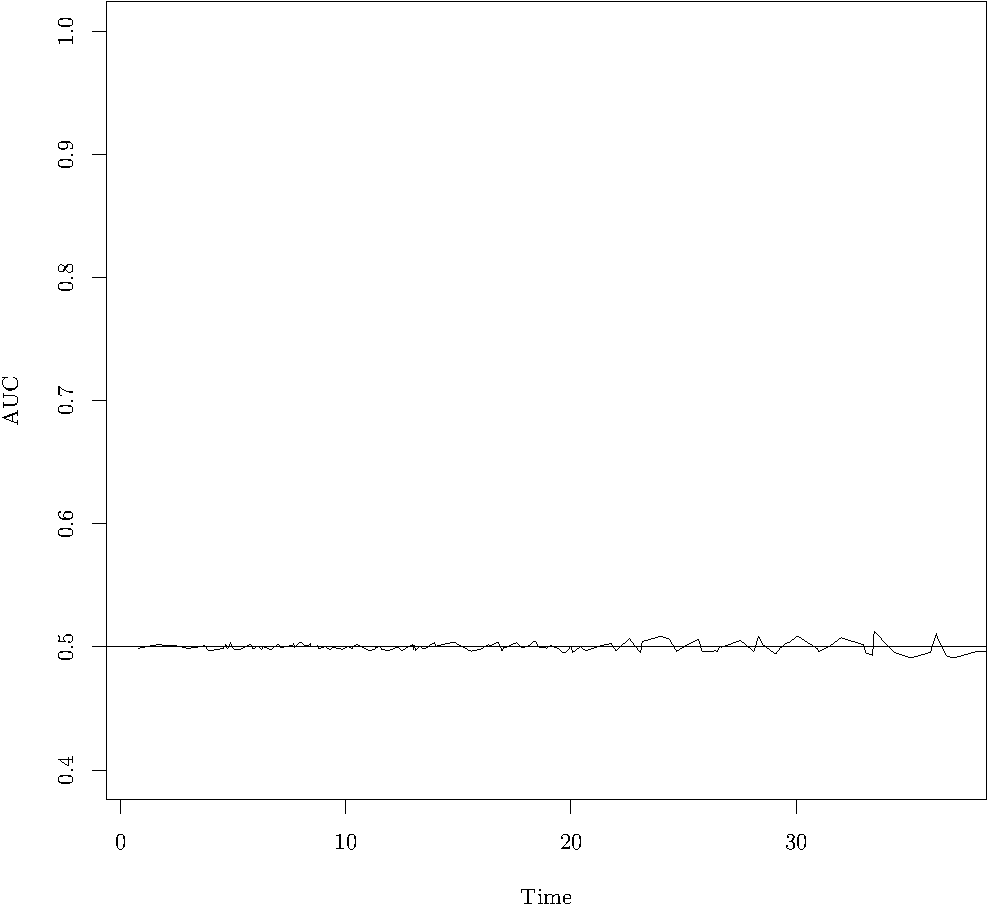
\includegraphics[width=\maxwidth]{figure/05-risksetROC-7} 

}


\begin{kframe}\begin{verbatim}
## $utimes
##   [1]   0.80   1.63   2.50   3.00   3.40   3.73   3.83   3.90   4.47   4.57
##  [11]   4.67   4.73   4.83   4.87   5.00   5.30   5.77   5.83   5.87   6.00
##  [21]   6.10   6.27   6.30   6.67   6.93   7.00   7.10   7.66   7.67   7.73
##  [31]   8.00   8.17   8.33   8.43   8.47   8.77   8.80   9.00   9.03   9.30
##  [41]   9.40   9.83  10.13  10.27  10.40  10.50  11.07  11.30  11.33  11.50
##  [51]  11.60  11.90  12.33  12.47  12.97  13.00  13.03  13.10  13.30  13.43
##  [61]  13.50  13.57  13.70  13.93  14.00  14.80  15.37  15.40  15.57  16.00
##  [71]  16.17  16.33  16.47  16.77  16.95  17.00  17.07  17.57  17.83  18.03
##  [81]  18.17  18.40  18.50  18.57  18.93  19.10  19.50  19.63  19.80  20.00
##  [91]  20.07  20.43  20.67  20.90  21.53  21.80  22.00  22.60  23.07  23.10
## [101]  23.17  24.00  24.37  24.70  25.00  25.67  25.83  26.33  26.40  26.50
## [111]  26.60  26.70  27.53  28.13  28.33  28.53  29.03  29.10  29.27  29.60
## [121]  29.67  30.07  30.97  31.00  31.53  32.00  33.00  33.10  33.40  33.47
## [131]  34.37  35.10  35.97  36.23  36.30  36.67  37.00  38.00  39.60  41.23
## [141]  43.07  45.37  46.67  47.43  47.73  48.00  49.00  51.00  54.90  59.00
## [151]  63.13  65.00  67.00  70.00  77.00  85.00  85.80  90.33  93.00  94.77
## [161] 116.00
## 
## $St
##   [1] 0.99476 0.98930 0.98383 0.97834 0.97284 0.96734 0.96185 0.95086
##   [9] 0.93986 0.93437 0.92887 0.92337 0.91788 0.90689 0.89589 0.89040
##  [17] 0.88490 0.87940 0.87391 0.86841 0.86291 0.85742 0.85192 0.84643
##  [25] 0.84093 0.83543 0.82994 0.82444 0.81894 0.81345 0.80246 0.79696
##  [33] 0.79146 0.78597 0.78047 0.77497 0.76948 0.76398 0.75845 0.75291
##  [41] 0.74737 0.74184 0.73630 0.73077 0.72523 0.71969 0.71416 0.70862
##  [49] 0.70308 0.69755 0.69201 0.68648 0.68094 0.67540 0.66987 0.66433
##  [57] 0.65880 0.65326 0.64772 0.64219 0.63665 0.63112 0.62558 0.62004
##  [65] 0.61451 0.60892 0.60333 0.59775 0.59216 0.58658 0.58099 0.57540
##  [73] 0.56982 0.56423 0.55864 0.55306 0.54747 0.54188 0.53630 0.53071
##  [81] 0.52512 0.51954 0.51395 0.50837 0.50278 0.49719 0.49161 0.48602
##  [89] 0.48043 0.46926 0.46367 0.45809 0.45250 0.44691 0.44133 0.43574
##  [97] 0.43016 0.42457 0.41898 0.41340 0.40781 0.39664 0.39105 0.38546
## [105] 0.37429 0.36870 0.36312 0.35753 0.35195 0.34636 0.34077 0.33519
## [113] 0.32960 0.32401 0.31843 0.31284 0.30725 0.30167 0.29608 0.29049
## [121] 0.28491 0.27932 0.27374 0.26815 0.26256 0.25698 0.25139 0.24580
## [129] 0.24022 0.23463 0.22904 0.22332 0.21759 0.21187 0.20614 0.20041
## [137] 0.19469 0.18289 0.17679 0.17048 0.16416 0.15760 0.15103 0.14446
## [145] 0.13790 0.13133 0.12442 0.11751 0.10967 0.10184 0.09401 0.08617
## [153] 0.07834 0.07050 0.06169 0.05141 0.04113 0.03085 0.02056 0.01028
## [161] 0.00000
## 
## $AUC
##   [1] 0.5723 0.5744 0.5766 0.5742 0.5699 0.5704 0.5729 0.5707 0.5694 0.5733
##  [11] 0.5701 0.5733 0.5732 0.5744 0.5792 0.5744 0.5699 0.5743 0.5718 0.5682
##  [21] 0.5726 0.5689 0.5701 0.5723 0.5692 0.5729 0.5689 0.5730 0.5732 0.5717
##  [31] 0.5680 0.5713 0.5724 0.5706 0.5709 0.5707 0.5726 0.5726 0.5719 0.5719
##  [41] 0.5776 0.5747 0.5700 0.5706 0.5736 0.5747 0.5754 0.5739 0.5752 0.5716
##  [51] 0.5735 0.5767 0.5744 0.5721 0.5778 0.5758 0.5791 0.5773 0.5717 0.5771
##  [61] 0.5716 0.5725 0.5753 0.5743 0.5760 0.5752 0.5759 0.5777 0.5774 0.5792
##  [71] 0.5811 0.5742 0.5734 0.5804 0.5796 0.5738 0.5759 0.5763 0.5778 0.5798
##  [81] 0.5771 0.5750 0.5825 0.5758 0.5784 0.5838 0.5812 0.5826 0.5830 0.5847
##  [91] 0.5817 0.5823 0.5862 0.5847 0.5791 0.5751 0.5844 0.5786 0.5805 0.5848
## [101] 0.5798 0.5749 0.5867 0.5802 0.5853 0.5819 0.5897 0.5834 0.5842 0.5865
## [111] 0.5923 0.5794 0.5826 0.5847 0.5876 0.5876 0.5839 0.5905 0.5831 0.5889
## [121] 0.5892 0.5848 0.5874 0.5882 0.5957 0.5881 0.5946 0.5966 0.6026 0.5892
## [131] 0.5956 0.6062 0.5856 0.5876 0.5931 0.5861 0.6086 0.6097 0.5945 0.5881
## [141] 0.6132 0.5807 0.5967 0.5913 0.5844 0.6111 0.5856 0.6234 0.6160 0.6236
## [151] 0.6229 0.5656 0.6111 0.6573 0.5917 0.5836 0.5309 0.4725 0.7439 0.2936
## [161] 0.0000
## 
## $Cindex
## [1] 0.576
\end{verbatim}
\begin{alltt}
\hlkwd{risksetAUC}\hlstd{(data.glasgow}\hlopt{$}\hlstd{Time}\hlopt{/}\hlnum{365.25}\hlopt{*}\hlnum{12}\hlstd{,} \hlkwc{status} \hlstd{= data.glasgow}\hlopt{$}\hlstd{DSD,} \hlkwc{marker} \hlstd{= gg.linpred.glasgow,} \hlkwc{tmax} \hlstd{=} \hlnum{36}\hlstd{)}
\end{alltt}
\end{kframe}

{\centering 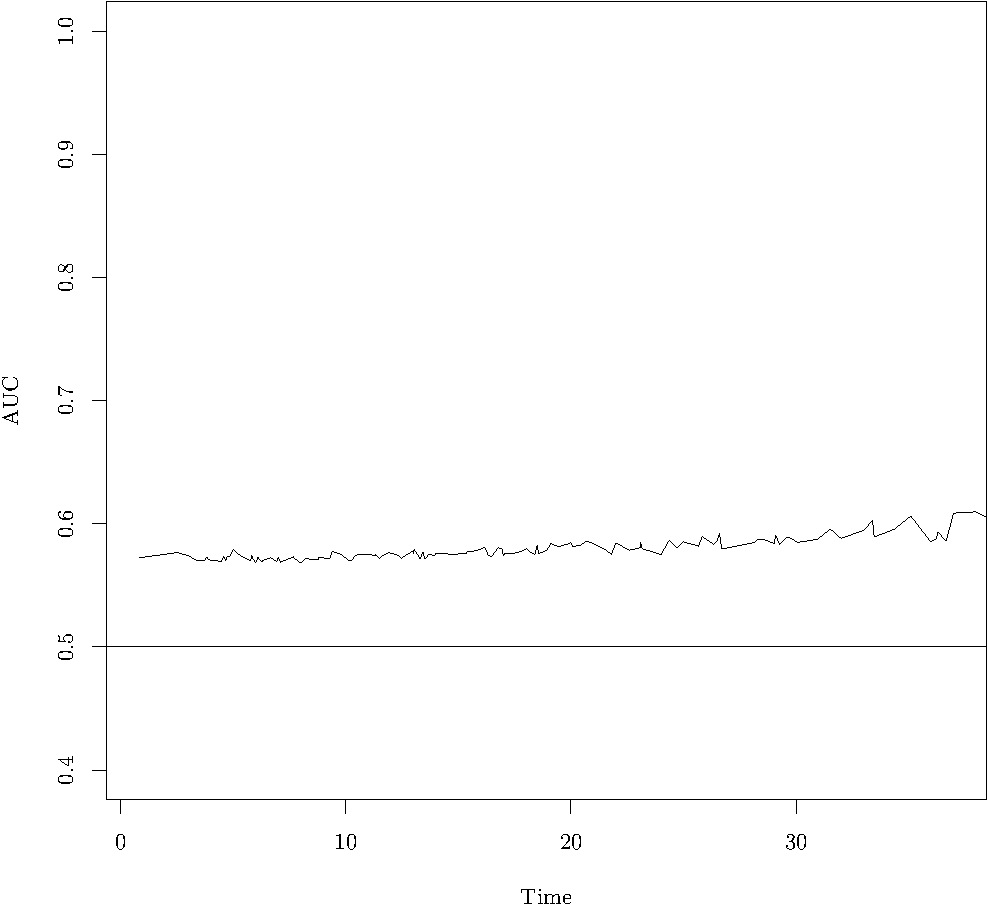
\includegraphics[width=\maxwidth]{figure/05-risksetROC-8} 

}


\begin{kframe}\begin{verbatim}
## $utimes
##   [1]   0.80   1.63   2.50   3.00   3.40   3.73   3.83   3.90   4.47   4.57
##  [11]   4.67   4.73   4.83   4.87   5.00   5.30   5.77   5.83   5.87   6.00
##  [21]   6.10   6.27   6.30   6.67   6.93   7.00   7.10   7.66   7.67   7.73
##  [31]   8.00   8.17   8.33   8.43   8.47   8.77   8.80   9.00   9.03   9.30
##  [41]   9.40   9.83  10.13  10.27  10.40  10.50  11.07  11.30  11.33  11.50
##  [51]  11.60  11.90  12.33  12.47  12.97  13.00  13.03  13.10  13.30  13.43
##  [61]  13.50  13.57  13.70  13.93  14.00  14.80  15.37  15.40  15.57  16.00
##  [71]  16.17  16.33  16.47  16.77  16.95  17.00  17.07  17.57  17.83  18.03
##  [81]  18.17  18.40  18.50  18.57  18.93  19.10  19.50  19.63  19.80  20.00
##  [91]  20.07  20.43  20.67  20.90  21.53  21.80  22.00  22.60  23.07  23.10
## [101]  23.17  24.00  24.37  24.70  25.00  25.67  25.83  26.33  26.40  26.50
## [111]  26.60  26.70  27.53  28.13  28.33  28.53  29.03  29.10  29.27  29.60
## [121]  29.67  30.07  30.97  31.00  31.53  32.00  33.00  33.10  33.40  33.47
## [131]  34.37  35.10  35.97  36.23  36.30  36.67  37.00  38.00  39.60  41.23
## [141]  43.07  45.37  46.67  47.43  47.73  48.00  49.00  51.00  54.90  59.00
## [151]  63.13  65.00  67.00  70.00  77.00  85.00  85.80  90.33  93.00  94.77
## [161] 116.00
## 
## $St
##   [1] 0.99476 0.98930 0.98383 0.97834 0.97284 0.96734 0.96185 0.95086
##   [9] 0.93986 0.93437 0.92887 0.92337 0.91788 0.90689 0.89589 0.89040
##  [17] 0.88490 0.87940 0.87391 0.86841 0.86291 0.85742 0.85192 0.84643
##  [25] 0.84093 0.83543 0.82994 0.82444 0.81894 0.81345 0.80246 0.79696
##  [33] 0.79146 0.78597 0.78047 0.77497 0.76948 0.76398 0.75845 0.75291
##  [41] 0.74737 0.74184 0.73630 0.73077 0.72523 0.71969 0.71416 0.70862
##  [49] 0.70308 0.69755 0.69201 0.68648 0.68094 0.67540 0.66987 0.66433
##  [57] 0.65880 0.65326 0.64772 0.64219 0.63665 0.63112 0.62558 0.62004
##  [65] 0.61451 0.60892 0.60333 0.59775 0.59216 0.58658 0.58099 0.57540
##  [73] 0.56982 0.56423 0.55864 0.55306 0.54747 0.54188 0.53630 0.53071
##  [81] 0.52512 0.51954 0.51395 0.50837 0.50278 0.49719 0.49161 0.48602
##  [89] 0.48043 0.46926 0.46367 0.45809 0.45250 0.44691 0.44133 0.43574
##  [97] 0.43016 0.42457 0.41898 0.41340 0.40781 0.39664 0.39105 0.38546
## [105] 0.37429 0.36870 0.36312 0.35753 0.35195 0.34636 0.34077 0.33519
## [113] 0.32960 0.32401 0.31843 0.31284 0.30725 0.30167 0.29608 0.29049
## [121] 0.28491 0.27932 0.27374 0.26815 0.26256 0.25698 0.25139 0.24580
## [129] 0.24022 0.23463 0.22904 0.22332 0.21759 0.21187 0.20614 0.20041
## [137] 0.19469 0.18289 0.17679 0.17048 0.16416 0.15760 0.15103 0.14446
## [145] 0.13790 0.13133 0.12442 0.11751 0.10967 0.10184 0.09401 0.08617
## [153] 0.07834 0.07050 0.06169 0.05141 0.04113 0.03085 0.02056 0.01028
## [161] 0.00000
## 
## $AUC
##   [1] 0.5807 0.5826 0.5803 0.5803 0.5791 0.5797 0.5773 0.5785 0.5788 0.5788
##  [11] 0.5816 0.5807 0.5806 0.5822 0.5823 0.5769 0.5824 0.5764 0.5798 0.5784
##  [21] 0.5777 0.5771 0.5807 0.5770 0.5816 0.5819 0.5766 0.5821 0.5808 0.5787
##  [31] 0.5838 0.5782 0.5791 0.5795 0.5777 0.5754 0.5743 0.5740 0.5756 0.5757
##  [41] 0.5747 0.5733 0.5737 0.5756 0.5756 0.5762 0.5743 0.5795 0.5792 0.5793
##  [51] 0.5733 0.5759 0.5744 0.5742 0.5808 0.5740 0.5798 0.5767 0.5735 0.5799
##  [61] 0.5748 0.5760 0.5796 0.5755 0.5737 0.5786 0.5737 0.5726 0.5725 0.5754
##  [71] 0.5789 0.5765 0.5784 0.5787 0.5732 0.5775 0.5759 0.5805 0.5802 0.5805
##  [81] 0.5813 0.5784 0.5830 0.5793 0.5739 0.5839 0.5721 0.5765 0.5812 0.5737
##  [91] 0.5728 0.5824 0.5769 0.5723 0.5752 0.5792 0.5717 0.5815 0.5701 0.5709
## [101] 0.5778 0.5879 0.5769 0.5667 0.5814 0.5728 0.5664 0.5689 0.5672 0.5659
## [111] 0.5773 0.5725 0.5717 0.5653 0.5801 0.5788 0.5625 0.5665 0.5715 0.5642
## [121] 0.5689 0.5706 0.5733 0.5669 0.5778 0.5839 0.5751 0.5607 0.5604 0.5787
## [131] 0.5555 0.5641 0.5719 0.5614 0.5639 0.5589 0.5577 0.5726 0.5561 0.5706
## [141] 0.5517 0.5854 0.5587 0.5572 0.5532 0.5497 0.5889 0.5654 0.5585 0.5384
## [151] 0.5967 0.5881 0.5616 0.5224 0.4994 0.5021 0.4551 0.4934 0.7081 0.7596
## [161] 0.0000
## 
## $Cindex
## [1] 0.5773
\end{verbatim}
\begin{alltt}
\hlkwd{risksetAUC}\hlstd{(data.glasgow}\hlopt{$}\hlstd{Time}\hlopt{/}\hlnum{365.25}\hlopt{*}\hlnum{12}\hlstd{,} \hlkwc{status} \hlstd{= data.glasgow}\hlopt{$}\hlstd{DSD,} \hlkwc{marker} \hlstd{= gg2.linpred.glasgow,} \hlkwc{tmax} \hlstd{=} \hlnum{36}\hlstd{)}
\end{alltt}
\end{kframe}

{\centering 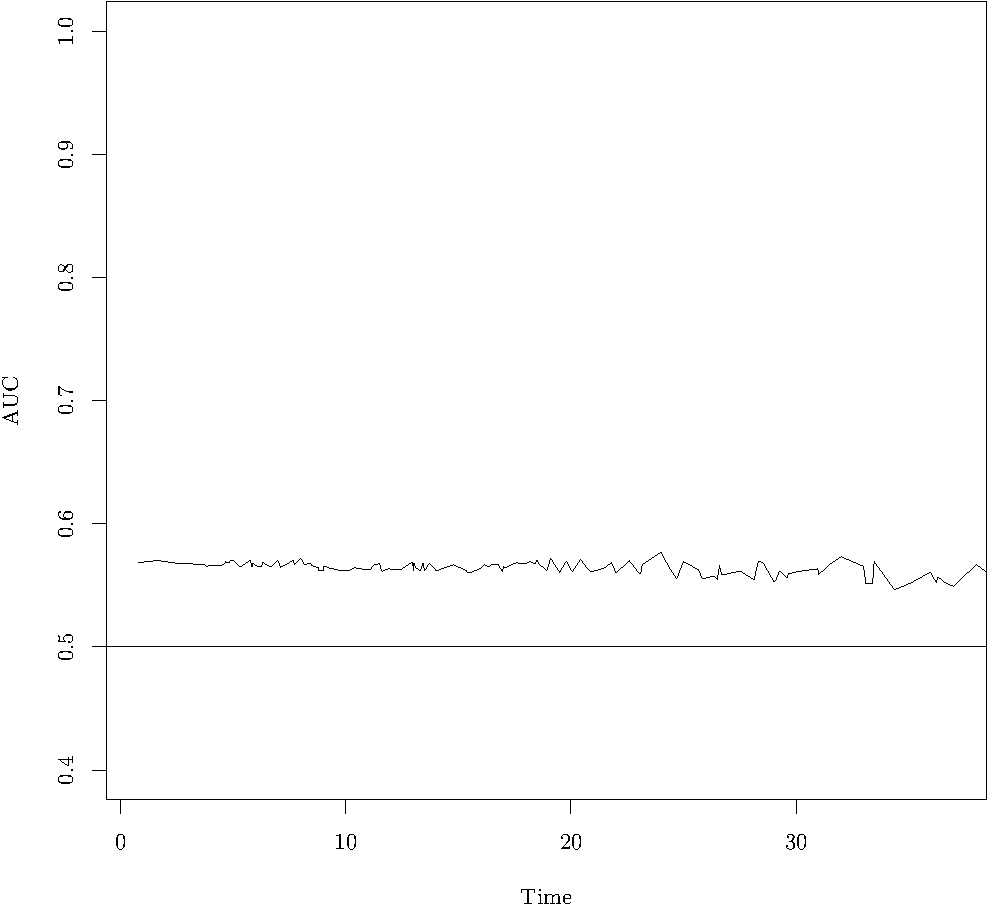
\includegraphics[width=\maxwidth]{figure/05-risksetROC-9} 

}


\begin{kframe}\begin{verbatim}
## $utimes
##   [1]   0.80   1.63   2.50   3.00   3.40   3.73   3.83   3.90   4.47   4.57
##  [11]   4.67   4.73   4.83   4.87   5.00   5.30   5.77   5.83   5.87   6.00
##  [21]   6.10   6.27   6.30   6.67   6.93   7.00   7.10   7.66   7.67   7.73
##  [31]   8.00   8.17   8.33   8.43   8.47   8.77   8.80   9.00   9.03   9.30
##  [41]   9.40   9.83  10.13  10.27  10.40  10.50  11.07  11.30  11.33  11.50
##  [51]  11.60  11.90  12.33  12.47  12.97  13.00  13.03  13.10  13.30  13.43
##  [61]  13.50  13.57  13.70  13.93  14.00  14.80  15.37  15.40  15.57  16.00
##  [71]  16.17  16.33  16.47  16.77  16.95  17.00  17.07  17.57  17.83  18.03
##  [81]  18.17  18.40  18.50  18.57  18.93  19.10  19.50  19.63  19.80  20.00
##  [91]  20.07  20.43  20.67  20.90  21.53  21.80  22.00  22.60  23.07  23.10
## [101]  23.17  24.00  24.37  24.70  25.00  25.67  25.83  26.33  26.40  26.50
## [111]  26.60  26.70  27.53  28.13  28.33  28.53  29.03  29.10  29.27  29.60
## [121]  29.67  30.07  30.97  31.00  31.53  32.00  33.00  33.10  33.40  33.47
## [131]  34.37  35.10  35.97  36.23  36.30  36.67  37.00  38.00  39.60  41.23
## [141]  43.07  45.37  46.67  47.43  47.73  48.00  49.00  51.00  54.90  59.00
## [151]  63.13  65.00  67.00  70.00  77.00  85.00  85.80  90.33  93.00  94.77
## [161] 116.00
## 
## $St
##   [1] 0.99476 0.98930 0.98383 0.97834 0.97284 0.96734 0.96185 0.95086
##   [9] 0.93986 0.93437 0.92887 0.92337 0.91788 0.90689 0.89589 0.89040
##  [17] 0.88490 0.87940 0.87391 0.86841 0.86291 0.85742 0.85192 0.84643
##  [25] 0.84093 0.83543 0.82994 0.82444 0.81894 0.81345 0.80246 0.79696
##  [33] 0.79146 0.78597 0.78047 0.77497 0.76948 0.76398 0.75845 0.75291
##  [41] 0.74737 0.74184 0.73630 0.73077 0.72523 0.71969 0.71416 0.70862
##  [49] 0.70308 0.69755 0.69201 0.68648 0.68094 0.67540 0.66987 0.66433
##  [57] 0.65880 0.65326 0.64772 0.64219 0.63665 0.63112 0.62558 0.62004
##  [65] 0.61451 0.60892 0.60333 0.59775 0.59216 0.58658 0.58099 0.57540
##  [73] 0.56982 0.56423 0.55864 0.55306 0.54747 0.54188 0.53630 0.53071
##  [81] 0.52512 0.51954 0.51395 0.50837 0.50278 0.49719 0.49161 0.48602
##  [89] 0.48043 0.46926 0.46367 0.45809 0.45250 0.44691 0.44133 0.43574
##  [97] 0.43016 0.42457 0.41898 0.41340 0.40781 0.39664 0.39105 0.38546
## [105] 0.37429 0.36870 0.36312 0.35753 0.35195 0.34636 0.34077 0.33519
## [113] 0.32960 0.32401 0.31843 0.31284 0.30725 0.30167 0.29608 0.29049
## [121] 0.28491 0.27932 0.27374 0.26815 0.26256 0.25698 0.25139 0.24580
## [129] 0.24022 0.23463 0.22904 0.22332 0.21759 0.21187 0.20614 0.20041
## [137] 0.19469 0.18289 0.17679 0.17048 0.16416 0.15760 0.15103 0.14446
## [145] 0.13790 0.13133 0.12442 0.11751 0.10967 0.10184 0.09401 0.08617
## [153] 0.07834 0.07050 0.06169 0.05141 0.04113 0.03085 0.02056 0.01028
## [161] 0.00000
## 
## $AUC
##   [1] 0.5685 0.5702 0.5679 0.5680 0.5666 0.5671 0.5650 0.5661 0.5665 0.5667
##  [11] 0.5694 0.5685 0.5683 0.5704 0.5701 0.5648 0.5704 0.5646 0.5678 0.5664
##  [21] 0.5654 0.5657 0.5686 0.5651 0.5697 0.5700 0.5647 0.5701 0.5690 0.5668
##  [31] 0.5719 0.5667 0.5675 0.5679 0.5663 0.5644 0.5620 0.5620 0.5657 0.5638
##  [41] 0.5636 0.5618 0.5621 0.5632 0.5644 0.5637 0.5626 0.5676 0.5670 0.5676
##  [51] 0.5614 0.5634 0.5625 0.5632 0.5690 0.5621 0.5680 0.5645 0.5616 0.5681
##  [61] 0.5621 0.5637 0.5678 0.5640 0.5617 0.5667 0.5617 0.5605 0.5606 0.5639
##  [71] 0.5669 0.5648 0.5669 0.5672 0.5610 0.5650 0.5643 0.5684 0.5674 0.5677
##  [81] 0.5693 0.5674 0.5708 0.5676 0.5620 0.5720 0.5604 0.5647 0.5696 0.5626
##  [91] 0.5613 0.5709 0.5651 0.5608 0.5644 0.5686 0.5602 0.5699 0.5589 0.5594
## [101] 0.5669 0.5769 0.5643 0.5553 0.5693 0.5627 0.5552 0.5574 0.5566 0.5548
## [111] 0.5661 0.5583 0.5616 0.5544 0.5695 0.5685 0.5525 0.5540 0.5617 0.5558
## [121] 0.5595 0.5612 0.5634 0.5587 0.5674 0.5732 0.5654 0.5513 0.5513 0.5693
## [131] 0.5464 0.5519 0.5607 0.5520 0.5570 0.5516 0.5491 0.5668 0.5466 0.5533
## [141] 0.5429 0.5764 0.5440 0.5500 0.5459 0.5409 0.5783 0.5370 0.5470 0.5256
## [151] 0.5821 0.5759 0.5498 0.5086 0.4861 0.4878 0.4420 0.4879 0.7018 0.7584
## [161] 0.0000
## 
## $Cindex
## [1] 0.5656
\end{verbatim}
\begin{alltt}
\hlkwd{risksetAUC}\hlstd{(data.glasgow}\hlopt{$}\hlstd{Time}\hlopt{/}\hlnum{365.25}\hlopt{*}\hlnum{12}\hlstd{,} \hlkwc{status} \hlstd{= data.glasgow}\hlopt{$}\hlstd{DSD,} \hlkwc{marker} \hlstd{= cph.linpred.glasgow,} \hlkwc{tmax} \hlstd{=} \hlnum{36}\hlstd{)}
\end{alltt}
\end{kframe}

{\centering 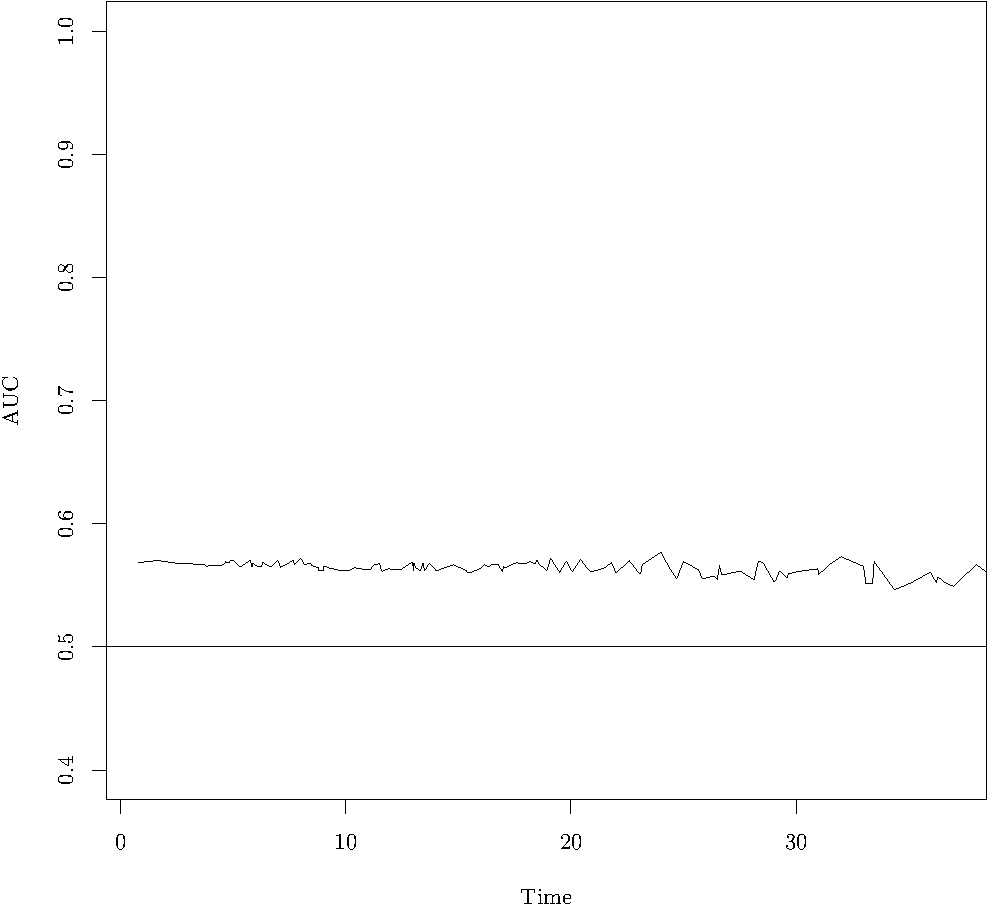
\includegraphics[width=\maxwidth]{figure/05-risksetROC-10} 

}


\begin{kframe}\begin{verbatim}
## $utimes
##   [1]   0.80   1.63   2.50   3.00   3.40   3.73   3.83   3.90   4.47   4.57
##  [11]   4.67   4.73   4.83   4.87   5.00   5.30   5.77   5.83   5.87   6.00
##  [21]   6.10   6.27   6.30   6.67   6.93   7.00   7.10   7.66   7.67   7.73
##  [31]   8.00   8.17   8.33   8.43   8.47   8.77   8.80   9.00   9.03   9.30
##  [41]   9.40   9.83  10.13  10.27  10.40  10.50  11.07  11.30  11.33  11.50
##  [51]  11.60  11.90  12.33  12.47  12.97  13.00  13.03  13.10  13.30  13.43
##  [61]  13.50  13.57  13.70  13.93  14.00  14.80  15.37  15.40  15.57  16.00
##  [71]  16.17  16.33  16.47  16.77  16.95  17.00  17.07  17.57  17.83  18.03
##  [81]  18.17  18.40  18.50  18.57  18.93  19.10  19.50  19.63  19.80  20.00
##  [91]  20.07  20.43  20.67  20.90  21.53  21.80  22.00  22.60  23.07  23.10
## [101]  23.17  24.00  24.37  24.70  25.00  25.67  25.83  26.33  26.40  26.50
## [111]  26.60  26.70  27.53  28.13  28.33  28.53  29.03  29.10  29.27  29.60
## [121]  29.67  30.07  30.97  31.00  31.53  32.00  33.00  33.10  33.40  33.47
## [131]  34.37  35.10  35.97  36.23  36.30  36.67  37.00  38.00  39.60  41.23
## [141]  43.07  45.37  46.67  47.43  47.73  48.00  49.00  51.00  54.90  59.00
## [151]  63.13  65.00  67.00  70.00  77.00  85.00  85.80  90.33  93.00  94.77
## [161] 116.00
## 
## $St
##   [1] 0.99476 0.98930 0.98383 0.97834 0.97284 0.96734 0.96185 0.95086
##   [9] 0.93986 0.93437 0.92887 0.92337 0.91788 0.90689 0.89589 0.89040
##  [17] 0.88490 0.87940 0.87391 0.86841 0.86291 0.85742 0.85192 0.84643
##  [25] 0.84093 0.83543 0.82994 0.82444 0.81894 0.81345 0.80246 0.79696
##  [33] 0.79146 0.78597 0.78047 0.77497 0.76948 0.76398 0.75845 0.75291
##  [41] 0.74737 0.74184 0.73630 0.73077 0.72523 0.71969 0.71416 0.70862
##  [49] 0.70308 0.69755 0.69201 0.68648 0.68094 0.67540 0.66987 0.66433
##  [57] 0.65880 0.65326 0.64772 0.64219 0.63665 0.63112 0.62558 0.62004
##  [65] 0.61451 0.60892 0.60333 0.59775 0.59216 0.58658 0.58099 0.57540
##  [73] 0.56982 0.56423 0.55864 0.55306 0.54747 0.54188 0.53630 0.53071
##  [81] 0.52512 0.51954 0.51395 0.50837 0.50278 0.49719 0.49161 0.48602
##  [89] 0.48043 0.46926 0.46367 0.45809 0.45250 0.44691 0.44133 0.43574
##  [97] 0.43016 0.42457 0.41898 0.41340 0.40781 0.39664 0.39105 0.38546
## [105] 0.37429 0.36870 0.36312 0.35753 0.35195 0.34636 0.34077 0.33519
## [113] 0.32960 0.32401 0.31843 0.31284 0.30725 0.30167 0.29608 0.29049
## [121] 0.28491 0.27932 0.27374 0.26815 0.26256 0.25698 0.25139 0.24580
## [129] 0.24022 0.23463 0.22904 0.22332 0.21759 0.21187 0.20614 0.20041
## [137] 0.19469 0.18289 0.17679 0.17048 0.16416 0.15760 0.15103 0.14446
## [145] 0.13790 0.13133 0.12442 0.11751 0.10967 0.10184 0.09401 0.08617
## [153] 0.07834 0.07050 0.06169 0.05141 0.04113 0.03085 0.02056 0.01028
## [161] 0.00000
## 
## $AUC
##   [1] 0.6364 0.6374 0.6358 0.6348 0.6322 0.6326 0.6292 0.6321 0.6324 0.6302
##  [11] 0.6310 0.6332 0.6319 0.6290 0.6321 0.6256 0.6308 0.6255 0.6304 0.6275
##  [21] 0.6268 0.6247 0.6302 0.6241 0.6276 0.6284 0.6250 0.6298 0.6277 0.6281
##  [31] 0.6294 0.6236 0.6255 0.6270 0.6241 0.6216 0.6233 0.6234 0.6225 0.6251
##  [41] 0.6210 0.6214 0.6223 0.6247 0.6219 0.6252 0.6228 0.6260 0.6294 0.6243
##  [51] 0.6206 0.6245 0.6229 0.6206 0.6270 0.6225 0.6258 0.6263 0.6214 0.6260
##  [61] 0.6237 0.6251 0.6249 0.6206 0.6230 0.6230 0.6221 0.6206 0.6213 0.6262
##  [71] 0.6245 0.6226 0.6246 0.6251 0.6226 0.6290 0.6219 0.6263 0.6305 0.6294
##  [81] 0.6247 0.6220 0.6274 0.6233 0.6213 0.6303 0.6198 0.6261 0.6261 0.6204
##  [91] 0.6230 0.6302 0.6277 0.6221 0.6192 0.6245 0.6210 0.6277 0.6202 0.6223
## [101] 0.6244 0.6355 0.6289 0.6152 0.6295 0.6147 0.6126 0.6194 0.6166 0.6150
## [111] 0.6283 0.6195 0.6110 0.6091 0.6231 0.6215 0.6095 0.6148 0.6108 0.6050
## [121] 0.6066 0.6078 0.6108 0.6056 0.6142 0.6253 0.6105 0.6061 0.6074 0.6204
## [131] 0.6008 0.6168 0.6239 0.6136 0.5999 0.6096 0.6064 0.6061 0.6068 0.6287
## [141] 0.6039 0.6359 0.6261 0.6045 0.6015 0.6116 0.6403 0.6405 0.6143 0.6478
## [151] 0.6759 0.6226 0.5906 0.5641 0.5829 0.5572 0.5140 0.5359 0.7544 0.7707
## [161] 0.0000
## 
## $Cindex
## [1] 0.6255
\end{verbatim}
\end{kframe}
\end{knitrout}

\end{document}
